% =====================================================================
% Kapitel 6 der Abteilungsvorlage, auf LaTeX übertragen.
% Vor der Abgabe komplett löschen: die Zeile % =====================================================================
% Kapitel 6 der Abteilungsvorlage, auf LaTeX übertragen.
% Vor der Abgabe komplett löschen: die Zeile % =====================================================================
% Kapitel 6 der Abteilungsvorlage, auf LaTeX übertragen.
% Vor der Abgabe komplett löschen: die Zeile % =====================================================================
% Kapitel 6 der Abteilungsvorlage, auf LaTeX übertragen.
% Vor der Abgabe komplett löschen: die Zeile \input{chapters/06-guideline}
% in diplomarbeit.tex entfernen und diese Datei mitlöschen.
% =====================================================================
\chapter{Richtlinie für das Verfassen von Diplomarbeiten}

Diese Richtlinie beschreibt die formalen und inhaltlichen Anforderungen an
eine wissenschaftliche Publikation und soll ein einheitliches
Erscheinungsbild der Diplomarbeiten sicherstellen. Dieses Kapitel beschreibt
weiters, wie die vorliegende Diplomarbeitsvorlage zu verwenden ist, und ist
im finalen Dokument zu entfernen.

Es sind bewusst nur die wesentlichen Punkte festgelegt. In Absprache mit dem
Betreuer/der Betreuerin soll stets Freiraum für die individuelle Gestaltung
sowie projektbedingte Erfordernisse bleiben.

\section{Allgemein}

Die Diplomarbeit soll kurz und prägnant -- aber vollständig -- gehalten sein
und einen Umfang von ca.\ 70 Seiten (ohne Anhang) bei einer Teamgröße von
2 Personen umfassen. Die inhaltliche Qualität bei in Umfang eingeschränkter
Darstellung ist ein wesentliches Ziel jeder wissenschaftlichen Publikation
und wird auch in die Beurteilung einbezogen. Grafische Darstellungen,
Übersichtstabellen und Diagramme sind wichtige Hilfsmittel, um diese Vorgabe
einhalten zu können.

Einige Tipps:

\begin{itemize}
  \item Das Verwenden der \enquote{ich}- und \enquote{wir}-Form sowie von
        \enquote{man}-Aussagen ist zu vermeiden.
  \item Abkürzungen müssen unmittelbar nach ihrem ersten Auftreten erläutert
        werden; falls erforderlich, ist ein Abkürzungsverzeichnis zu
        erstellen. Der Befehl \lstinline|\ac{API}| erledigt das automatisch:
        beim ersten Auftreten schreibt er die Abkürzung aus, danach nicht
        mehr.
  \item Über Themen, die nur indirekt mit der gestellten Aufgabe zu tun
        haben, soll nicht berichtet werden. Die ausführliche Darstellung von
        Grundlagenwissen ist nicht erforderlich; meistens reicht das Zitieren
        geeigneter Quellen.
  \item Arbeitet im Team über ein Git-Repository und legt pro Kapitel eine
        eigene Datei an. So lassen sich Änderungen nachvollziehen und
        Konflikte auf einzelne Absätze eingrenzen.
\end{itemize}

\subsection{Platzhalter in dieser Vorlage}

Alle Beispieltexte in dieser Vorlage sind zu ersetzen oder zu löschen. Das
betrifft insbesondere:

\begin{itemize}
  \item die Metadaten in \lstinline|metadata.tex| (Titel, Team, Betreuung,
        Schuljahr, Klasse),
  \item die Beispielkapitel in \lstinline|chapters/|,
  \item die Beispielquellen in \lstinline|references.bib|,
  \item das Abkürzungsverzeichnis in \lstinline|diplomarbeit.tex|,
  \item dieses gesamte Kapitel~6.
\end{itemize}

Um dieses Kapitel zu entfernen, genügt es, in \lstinline|diplomarbeit.tex|
die Zeile \lstinline|\input{chapters/06-guideline}| zu löschen. Die Einträge
im Inhaltsverzeichnis und in den übrigen Verzeichnissen verschwinden beim
nächsten Übersetzen von selbst.

\subsection{Abgabe der Diplomarbeit}

Die Diplomarbeit ist in gedruckter bzw.\ gebundener Form und in digitaler
Form vorzulegen. Dem Abteilungsvorstand sind zwei geheftete Exemplare (ein
Belegexemplar und ein Beurteilungsexemplar für den/die Betreuer/in) zu
übergeben.

Nach erfolgter Beurteilung geht das Beurteilungsexemplar temporär zurück an
die Diplomarbeitsgruppe. Nun können letzte Korrekturen (ohne
Beurteilungsrelevanz) vorgenommen werden. Anschließend wird die Arbeit erneut
ausgedruckt und gesammelt zur Bindung außer Haus gegeben. Weitere Exemplare
für Kooperationspartner (Firmen, Institutionen) oder Projektteilnehmer können
in diesem Zusammenhang erstellt werden.

\subsection{Grafiken}

Abbildungen müssen in gut lesbarer Bildqualität eingefügt werden. Grafiken
sollten am besten in einem vektorbasierten Zeichenprogramm (z.\,B. Inkscape,
draw.io) erstellt und als PDF exportiert werden; PDF und PNG lassen sich
direkt einbinden, SVG nicht. Alle Bilddateien gehören in den Ordner
\lstinline|images/|.

\begin{lstlisting}[language={[LaTeX]TeX}, caption={Eine Abbildung einbinden},
                   label=code:abbildung]
\begin{figure}[htbp]
  \centering
  
\includegraphics[width=0.75\linewidth]{images/example-figure.pdf}
  \caption{Aufbau des Systems}
  \label{abb:aufbau}
\end{figure}
\end{lstlisting}

Abb.~\ref{abb:blue-marble} zeigt, wie das Ergebnis aussieht. Stammt die
Grafik nicht von euch selbst, gehört die Quelle in die Beschriftung.

\begin{figure}[htbp]
  \centering
  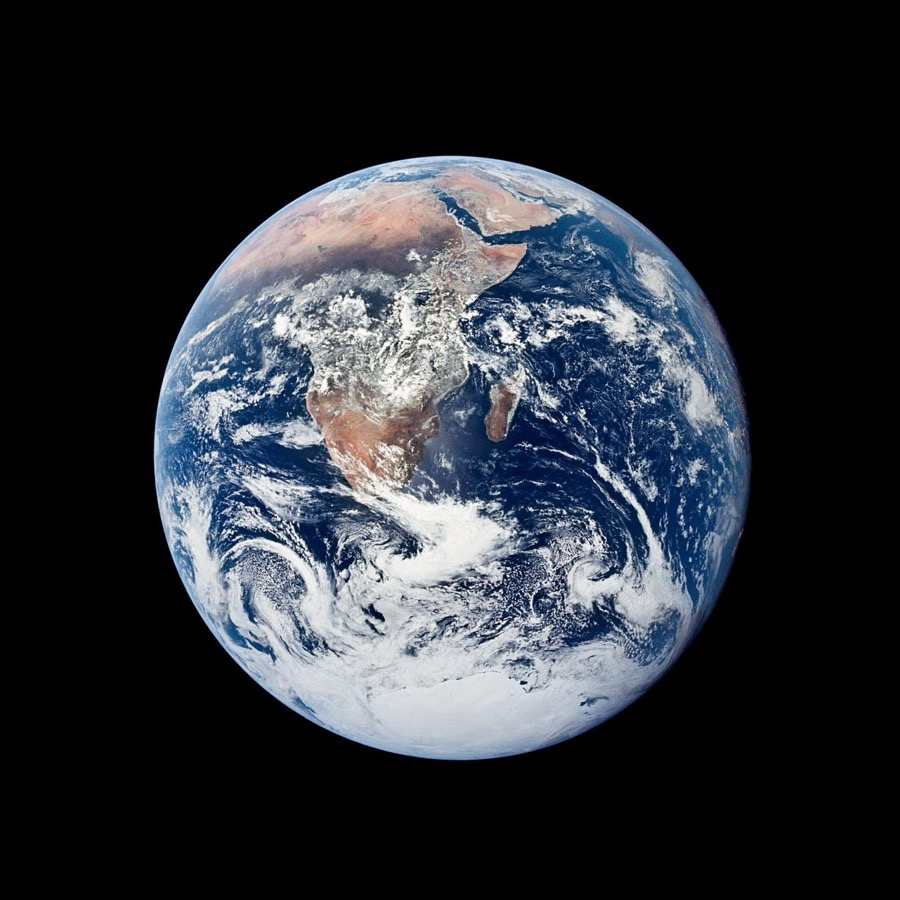
\includegraphics[width=0.55\linewidth]{images/blue-marble-nasa.jpg}
  \caption{Beispielabbildung mit Quellenangabe~\cite{nasa-blue-marble}}
  \label{abb:blue-marble}
\end{figure}

Vektorgrafiken haben gegenüber Screenshots den Vorteil, dass

\begin{itemize}
  \item sie jederzeit editiert werden können,
  \item sie beliebig skaliert werden können, ohne unscharf zu werden,
  \item alle Grafiken einheitlich vergrößert oder verkleinert werden können.
        Das verbessert das Layout ungemein.
\end{itemize}

Abbildungen stehen immer alleinstehend und zentriert. Die Breite wird
relativ zur Textbreite angegeben (\lstinline|width=0.75\linewidth|), damit
sie nie über den Satzspiegel hinausragt. Sollen mehrere Grafiken
nebeneinander stehen, verwendet dafür zwei \lstinline|minipage|-Umgebungen
innerhalb einer \lstinline|figure|.

Die Positionierung übernimmt \LaTeX. Die Angabe \lstinline|[htbp]| erlaubt
es, die Abbildung an die Stelle im Text, an den Seitenanfang, an das
Seitenende oder auf eine eigene Seite zu setzen. Eine Abbildung kann dadurch
auf der Folgeseite landen -- das ist beabsichtigt und kein Fehler.

\subsection{Beschriftungen}

Alle Grafiken und Tabellen sind zu beschriften und mit Quellenangaben zu
versehen. Im Text muss auf jede Abbildung und jede Tabelle Bezug genommen
werden.

Die Beschriftung erfolgt mit \lstinline|\caption| innerhalb der
\lstinline|figure|- bzw.\ \lstinline|table|-Umgebung. Nur so werden
Abbildungs- und Tabellenverzeichnis korrekt geführt. Bei Abbildungen steht
die Beschriftung unter der Grafik, bei Tabellen darüber; die Vorlage stellt
das automatisch richtig ein.

Abbildungen werden mit \enquote{Abb.} und Tabellen mit \enquote{Tab.}
bezeichnet. Auch das erledigt die Vorlage; die Nummerierung läuft
durchgehend und nicht kapitelweise. In englischsprachigen Diplomarbeiten
wird \enquote{Abb.} durch \enquote{Fig.} ersetzt -- dafür genügt die
Klassenoption \lstinline|englisch|.

Unmittelbar nach \lstinline|\caption| gehört ein \lstinline|\label|. Ohne
Label lässt sich die Abbildung später nicht referenzieren. Bewährt hat sich
ein Präfix je Objektart: \lstinline|abb:|, \lstinline|tab:| und
\lstinline|code:|.

\subsection{Querverweise}

Textpassagen, die sich auf andere Kapitel, Grafiken oder Tabellen beziehen,
müssen eine Referenz enthalten. Diese wird mit \lstinline|\ref| erzeugt und
enthält zumindest die Kategorie und die Nummer, also etwa
\lstinline|Abb.~\ref{abb:aufbau}|. Das geschützte Leerzeichen
\lstinline|~| verhindert, dass zwischen Bezeichnung und Nummer umgebrochen
wird.

Liegen referenzierender Text und referenziertes Objekt mehr als eine Seite
auseinander, ist zusätzlich die Seitenzahl mit \lstinline|\pageref|
anzugeben.

Anders als in Word müssen Querverweise und Verzeichnisse nicht manuell
aktualisiert werden. \LaTeX{} löst sie beim Übersetzen auf, benötigt dafür
aber mehrere Durchläufe. \lstinline|latexmk| (bzw.\ \lstinline|make pdf|)
wiederholt den Lauf so lange, bis sich nichts mehr ändert. Meldet das
Protokoll am Ende \enquote{There were undefined references}, fehlt ein
\lstinline|\label| oder es ist falsch geschrieben.

\subsection{Quellenangaben}

In wissenschaftlichen Arbeiten ist es verpflichtend, die Quelle jeder
Aussage anzugeben, die nicht von einem selbst stammt. Der Leser muss die
Möglichkeit haben, die Ausführungen des Autors nachzuprüfen.

Zu diesem Zweck müssen im Text der Diplomarbeit alle verwendeten Quellen
(Fachbücher, Fachzeitschriften, Herstellerunterlagen, Webseiten, \ldots)
angegeben werden. Dies geschieht am Ende des zitierten Textes durch Angabe
der Quelle. Informationen aus Lehrbüchern können als Allgemeinwissen
vorausgesetzt werden und müssen nicht zitiert werden.

Bei inhaltlichen Zitaten, dem Normalfall in technischen Arbeiten, wird der
Inhalt der Quelle nur sinngemäß wiedergegeben.

Bei wörtlichen Zitaten, die in technischen Arbeiten eher selten auftreten,
wird die wörtlich zitierte Textstelle zwischen Anführungszeichen gesetzt,
dahinter steht die Quellenangabe. Eigene Kommentare im Zitat oder
Verkürzungen werden in eckigen Klammern angegeben. Kurze Zitate stehen mit
\lstinline|\zitat| im Fließtext, längere in der Umgebung
\lstinline|zitatfreistehend|.

Beispiel für ein Zitat im Text der Diplomarbeit:
\zitat{[\ldots] kann in diesem Fall eine relationale Datenbank vorteilhaft
eingesetzt werden}~\cite{beispiel-buch}.

Beispiel für ein Zitat als eigener Absatz:

\begin{zitatfreistehend}
  \enquote{The basic guideline for citing online sources is to follow the
  standard citation for the citation, or add the DOI in place of page
  numbers if the source is not paginated.}~\cite{beispiel-artikel}
\end{zitatfreistehend}

Für Diplomarbeiten an der \ac{HTL} Donaustadt ist der IEEE-Zitierstil zu
verwenden. Jeder Quelle wird eine Nummer zugeordnet und in eckigen Klammern
angegeben. Diese Vorlage stellt den Stil bereits ein; zitiert wird mit
\lstinline|\cite{schluessel}|, wobei der Schlüssel aus
\lstinline|references.bib| stammt. Das Quellenverzeichnis wird daraus
automatisch erzeugt und enthält nur tatsächlich zitierte Einträge.

Zum Verwalten der Quellen empfiehlt sich Zotero mit dem Plug-in Better
BibTeX, das \lstinline|references.bib| bei jeder Änderung automatisch neu
exportiert.

Es gibt viele verschiedene Typen von Quellen. Tab.~\ref{tab:quellentypen}
zeigt die häufigsten, den passenden BibTeX-Eintragstyp und die
Informationen, die mindestens enthalten sein sollten.

\begin{table}[htbp]
  \centering
  \caption{Quellentypen}
  \label{tab:quellentypen}
  \begin{tabular}{@{}p{0.28\linewidth}p{0.16\linewidth}p{0.46\linewidth}@{}}
    \toprule
    \tabkopf{Quellentyp} & \tabkopf{Eintragstyp} &
      \tabkopf{wichtigste Informationen} \\
    \midrule
    Buch (auch E-Books, Broschüren) & \lstinline|@book| &
      Autor(en), Titel, Auflage, Verlag, Ort, ISBN \\
    Diplomarbeit, Dissertation & \lstinline|@thesis| &
      Autor(en), Titel, Institution, Ort, Datum \\
    Webseite (auch PDF) & \lstinline|@online| &
      Autor(en), Titel, URL, Abrufdatum (\lstinline|urldate|) \\
    Zeitschriftenartikel & \lstinline|@article| &
      Autor(en), Titel, Publikation, Band, Ausgabe, Seiten, Datum \\
    Verwendung von KI & \lstinline|@online| &
      siehe Anhang und die Vorgaben des Ministeriums~\cite{beispiel-online} \\
    \bottomrule
  \end{tabular}
\end{table}

\subsection{Befehle und Umgebungen}

In Word übernehmen Formatvorlagen das einheitliche Layout. In \LaTeX{}
erfüllen Befehle und Umgebungen dieselbe Aufgabe: Der Text beschreibt, was
etwas \emph{ist}, das Aussehen legt die Dokumentklasse \lstinline|htldon.cls|
zentral fest. Dadurch lässt sich die Formatierung nachträglich an einer
einzigen Stelle ändern.

Die in Tab.~\ref{tab:befehle} aufgeführten Befehle stellen sicher, dass alle
Diplomarbeiten den Richtlinien entsprechen. Sie dürfen nur in begründeten
Ausnahmefällen angepasst werden.

\begin{table}[htbp]
  \centering
  \caption{Befehle und Umgebungen der Vorlage}
  \label{tab:befehle}
  \begin{tabular}{@{}p{0.36\linewidth}p{0.58\linewidth}@{}}
    \toprule
    \tabkopf{Befehl} & \tabkopf{Beschreibung} \\
    \midrule
    \lstinline|\chapter| bis \lstinline|\subsubsection| &
      Kapitelüberschriften mit Dezimalklassifikation. Die ersten drei Ebenen
      erscheinen im Inhaltsverzeichnis, \lstinline|\subsubsection| nicht. \\
    \lstinline|\paragraph| &
      Zwischenüberschrift ohne Nummerierung, nicht im Inhaltsverzeichnis. \\
    \lstinline|\abschnittsautor| &
      Verfasser/in eines Abschnitts, erscheint rechts in der Kopfzeile.
      Format: erster Buchstabe des Vornamens, Punkt, Nachname
      (\enquote{M. Muster}). \\
    \lstinline|\zitat|, \lstinline|zitatfreistehend| &
      Kennzeichnung wörtlicher Zitate im Fließtext bzw.\ als eigener Absatz. \\
    \lstinline|\menue| &
      Menüstrukturen (\menue{Datei / Öffnen}) und Tastatureingaben
      (\menue{Strg + A}). \\
    \lstinline|lstlisting|, \lstinline|\lstinline| &
      Quellcode als eigener Block bzw.\ im Fließtext. \\
    \lstinline|\tabkopf| &
      Kopfzeile einer Tabelle. Der Tabelleninhalt selbst wird von der Klasse
      automatisch auf 10\,pt und linksbündig gestellt. \\
    \lstinline|\ac|, \lstinline|\acp| &
      Abkürzung, beim ersten Auftreten ausgeschrieben, im Plural mit
      \lstinline|\acp|. \\
    \lstinline|\cite|, \lstinline|\ref|, \lstinline|\pageref| &
      Quellenangabe, Querverweis, Seitenverweis. \\
    \bottomrule
  \end{tabular}
\end{table}

Überschriften der Kapitel müssen kurz, präzise und selbsterklärend sein.
Beispiele für unzureichende Überschriften: \enquote{5.3 Aufbau},
\enquote{5.3 Messergebnis}, \enquote{5.3 Beispiel}.

Bei Unterüberschriften gilt:

\begin{itemize}
  \item Es muss mindestens zwei Unterpunkte geben. Ein Abschnitt 3.2.1 darf
        daher nicht existieren, wenn kein 3.2.2 folgt.
  \item Unterpunkte sollten inhaltlich ausreichend gefüllt sein und
        mindestens eine halbe Seite umfassen.
  \item Unterpunkte, die lediglich aus einem einzelnen Satz bestehen, werden
        besser als Aufzählung dargestellt.
\end{itemize}

Für die Darstellung von Quellcode gilt:

\begin{itemize}
  \item Umfang:
        \begin{itemize}
          \item Der vollständige Sourcecode gehört ausschließlich auf das
                elektronische Speichermedium.
          \item Im Dokument selbst sollen nur wesentliche Ausschnitte
                aufgenommen werden.
        \end{itemize}
  \item Formatierung: Schriftart und Schriftgröße gibt die
        \lstinline|lstlisting|-Umgebung vor, der Zeilenabstand ist dort
        einzeilig. Die Sprache wird mit
        \lstinline|[language=Python]| angegeben, damit die
        Syntaxhervorhebung stimmt.
  \item Inhaltliche Anforderungen: Der Sourcecode muss ausreichend
        kommentiert sein.
  \item Verwendung im Fließtext: Wird Sourcecode im Text erwähnt, ist
        \lstinline|\lstinline| zu verwenden. Zusätzliche Anführungszeichen
        sind nicht erforderlich. Beispiel: Mit dem Befehl
        \lstinline|ShowModal| wird ein Frame geöffnet.
\end{itemize}

\section{Beschreibung der Kapitel}

\subsection{Titelseite}

Die Titelseite wird vollständig aus \lstinline|metadata.tex| erzeugt. Dort
sind einzutragen:

\begin{itemize}
  \item der Titel der Diplomarbeit mit \lstinline|\titel|. Er wird
        automatisch in die Kopfzeile übernommen.
  \item ein Projektlogo, Bild oder eine Zeichnung mit
        \lstinline|\projektlogo|.
  \item alle Verfasser/innen mit \lstinline|\teammitglied| und die
        Betreuung mit \lstinline|\betreuung|.
  \item Schuljahr, Abteilung und Klasse.
\end{itemize}

Falls alle Verfasser/innen oder Betreuer/innen dasselbe Geschlecht haben,
kann die geschlechtsspezifische Form verwendet werden; dafür ist das
optionale Argument von \lstinline|\betreuung| vorgesehen.

\subsection{Verfassererklärung}

In der Verfassererklärung bekennen sich die Verfasser/innen zu einem
wissenschaftlichen Arbeitsstil. Sollten im Nachhinein grobe Verstöße dagegen
aufgedeckt werden, kann die Arbeit für ungültig erklärt und der Abschluss
revidiert werden.

Die Erklärung erzeugt \lstinline|\eigenstaendigkeitserklaerung|. Je
Teammitglied entsteht automatisch eine Unterschriftszeile. Zu ergänzen sind
gegebenenfalls Kooperationen mit Firmen und Sperrvermerke.

\subsection{Problemstellung}

Die Seite \enquote{Problemstellung} wird durch den eingescannten Antrag (mit
allen Stempeln und Unterschriften) vollflächig ersetzt. Dazu wird in
\lstinline|frontmatter/problem-statement.tex| das Scan-PDF eingebunden.

\subsection{Kurzfassung bzw.\ Abstract}

Die Kurzfassung bzw.\ der Abstract soll kurz, prägnant und verständlich den
Inhalt der Arbeit wiedergeben: Zielsetzung, Ablauf, wichtigste Erkenntnisse,
wesentliche Merkmale des realisierten Produkts, Schlussfolgerungen und
Ausblick. Beide sind als eigenständiges Dokument zu konzipieren, das
unabhängig von der Diplomarbeit gelesen und verstanden werden kann, und
sollen in Deutsch und Englisch jeweils nicht mehr als eine Seite umfassen.

\subsection{Inhaltsverzeichnis}

Das Inhaltsverzeichnis wird automatisch aus den Überschriften erstellt. Es
zeigt die ersten drei Ebenen, der Text steht linksbündig, die Seitenzahlen
rechtsbündig, als Füllzeichen dienen Punkte. Eine manuelle Aktualisierung
ist nicht nötig.

\subsection{Die weiteren Kapitel}

Die Kapitel Projektplanung, Technische Grundlagen, Praktische Realisierung
sowie Evaluierung und Ergebnisse beschreiben die Diplomarbeit im Detail.

Für die Beurteilung ist es wichtig, den/die Verfasser/in zu kennen. Daher
ist dieser Hinweis auf jeder Seite rechtsbündig in der Kopfzeile zu
vermerken. Dafür wird \lstinline|\abschnittsautor| direkt nach der
Überschrift gesetzt; der Eintrag gilt ab dort bis zur nächsten Angabe.
Haben mehrere Personen gemeinsam an einem Abschnitt gearbeitet, sind alle zu
nennen, durch Komma getrennt:
\lstinline|\abschnittsautor{A. Erste, B. Zweite}|.

Die Projektplanung soll die systematische Durchführung der Diplomarbeit
innerhalb des Projektteams beschreiben. Dabei sollen geplante Ziele und
tatsächlich erreichte Ergebnisse miteinander verglichen und die Unterschiede
reflektiert werden. Beim klassischen Wasserfall-Projektmanagement können
etwa die Meilensteine als Referenz dienen, bei agiler Projektorganisation
die Sprint-Reviews.

Im Kapitel Technische Grundlagen finden sich alle für das unmittelbare
technische Verständnis der Diplomarbeit relevanten Inhalte. Hier wird
insbesondere auf korrekte Zitate und den sorgfältigen Einsatz von Quellen
geachtet.

Das Kapitel Praktische Realisierung enthält die praktischen Eigenleistungen
der Diplomarbeit. Dabei sollen die Vorgänge und Untersuchungen beschrieben
und nachvollziehbar dokumentiert werden.

Im Kapitel Evaluierung und Ergebnisse erfolgt die Darstellung und Bewertung
der abschließenden Arbeit. Hier soll ebenso, sofern vorhanden, das
Endprodukt bzw.\ der Prototyp präsentiert und beschrieben werden.

\subsection{Anhang}

Im Anhang können alle Informationen gesammelt werden, die zwar zur
Diplomarbeit gehören, jedoch im Inhaltsteil den Rahmen gesprengt hätten.
Dazu zählen wichtige Notizen (z.\,B. Gesprächsprotokolle), Normen,
Schnittstellendefinitionen oder Präsentationen. Weiters soll der Anhang den
Inhalt eines beigefügten elektronischen Speichermediums sowie einen
einseitigen Lebenslauf jedes Teammitglieds enthalten.

Verpflichtend ist außerdem die Dokumentation aller eingesetzten KI-basierten
Hilfsmittel. Dafür ist \lstinline|appendix/ai-tools.tex| vorgesehen.

% in diplomarbeit.tex entfernen und diese Datei mitlöschen.
% =====================================================================
\chapter{Richtlinie für das Verfassen von Diplomarbeiten}

Diese Richtlinie beschreibt die formalen und inhaltlichen Anforderungen an
eine wissenschaftliche Publikation und soll ein einheitliches
Erscheinungsbild der Diplomarbeiten sicherstellen. Dieses Kapitel beschreibt
weiters, wie die vorliegende Diplomarbeitsvorlage zu verwenden ist, und ist
im finalen Dokument zu entfernen.

Es sind bewusst nur die wesentlichen Punkte festgelegt. In Absprache mit dem
Betreuer/der Betreuerin soll stets Freiraum für die individuelle Gestaltung
sowie projektbedingte Erfordernisse bleiben.

\section{Allgemein}

Die Diplomarbeit soll kurz und prägnant -- aber vollständig -- gehalten sein
und einen Umfang von ca.\ 70 Seiten (ohne Anhang) bei einer Teamgröße von
2 Personen umfassen. Die inhaltliche Qualität bei in Umfang eingeschränkter
Darstellung ist ein wesentliches Ziel jeder wissenschaftlichen Publikation
und wird auch in die Beurteilung einbezogen. Grafische Darstellungen,
Übersichtstabellen und Diagramme sind wichtige Hilfsmittel, um diese Vorgabe
einhalten zu können.

Einige Tipps:

\begin{itemize}
  \item Das Verwenden der \enquote{ich}- und \enquote{wir}-Form sowie von
        \enquote{man}-Aussagen ist zu vermeiden.
  \item Abkürzungen müssen unmittelbar nach ihrem ersten Auftreten erläutert
        werden; falls erforderlich, ist ein Abkürzungsverzeichnis zu
        erstellen. Der Befehl \lstinline|\ac{API}| erledigt das automatisch:
        beim ersten Auftreten schreibt er die Abkürzung aus, danach nicht
        mehr.
  \item Über Themen, die nur indirekt mit der gestellten Aufgabe zu tun
        haben, soll nicht berichtet werden. Die ausführliche Darstellung von
        Grundlagenwissen ist nicht erforderlich; meistens reicht das Zitieren
        geeigneter Quellen.
  \item Arbeitet im Team über ein Git-Repository und legt pro Kapitel eine
        eigene Datei an. So lassen sich Änderungen nachvollziehen und
        Konflikte auf einzelne Absätze eingrenzen.
\end{itemize}

\subsection{Platzhalter in dieser Vorlage}

Alle Beispieltexte in dieser Vorlage sind zu ersetzen oder zu löschen. Das
betrifft insbesondere:

\begin{itemize}
  \item die Metadaten in \lstinline|metadata.tex| (Titel, Team, Betreuung,
        Schuljahr, Klasse),
  \item die Beispielkapitel in \lstinline|chapters/|,
  \item die Beispielquellen in \lstinline|references.bib|,
  \item das Abkürzungsverzeichnis in \lstinline|diplomarbeit.tex|,
  \item dieses gesamte Kapitel~6.
\end{itemize}

Um dieses Kapitel zu entfernen, genügt es, in \lstinline|diplomarbeit.tex|
die Zeile \lstinline|% =====================================================================
% Kapitel 6 der Abteilungsvorlage, auf LaTeX übertragen.
% Vor der Abgabe komplett löschen: die Zeile \input{chapters/06-guideline}
% in diplomarbeit.tex entfernen und diese Datei mitlöschen.
% =====================================================================
\chapter{Richtlinie für das Verfassen von Diplomarbeiten}

Diese Richtlinie beschreibt die formalen und inhaltlichen Anforderungen an
eine wissenschaftliche Publikation und soll ein einheitliches
Erscheinungsbild der Diplomarbeiten sicherstellen. Dieses Kapitel beschreibt
weiters, wie die vorliegende Diplomarbeitsvorlage zu verwenden ist, und ist
im finalen Dokument zu entfernen.

Es sind bewusst nur die wesentlichen Punkte festgelegt. In Absprache mit dem
Betreuer/der Betreuerin soll stets Freiraum für die individuelle Gestaltung
sowie projektbedingte Erfordernisse bleiben.

\section{Allgemein}

Die Diplomarbeit soll kurz und prägnant -- aber vollständig -- gehalten sein
und einen Umfang von ca.\ 70 Seiten (ohne Anhang) bei einer Teamgröße von
2 Personen umfassen. Die inhaltliche Qualität bei in Umfang eingeschränkter
Darstellung ist ein wesentliches Ziel jeder wissenschaftlichen Publikation
und wird auch in die Beurteilung einbezogen. Grafische Darstellungen,
Übersichtstabellen und Diagramme sind wichtige Hilfsmittel, um diese Vorgabe
einhalten zu können.

Einige Tipps:

\begin{itemize}
  \item Das Verwenden der \enquote{ich}- und \enquote{wir}-Form sowie von
        \enquote{man}-Aussagen ist zu vermeiden.
  \item Abkürzungen müssen unmittelbar nach ihrem ersten Auftreten erläutert
        werden; falls erforderlich, ist ein Abkürzungsverzeichnis zu
        erstellen. Der Befehl \lstinline|\ac{API}| erledigt das automatisch:
        beim ersten Auftreten schreibt er die Abkürzung aus, danach nicht
        mehr.
  \item Über Themen, die nur indirekt mit der gestellten Aufgabe zu tun
        haben, soll nicht berichtet werden. Die ausführliche Darstellung von
        Grundlagenwissen ist nicht erforderlich; meistens reicht das Zitieren
        geeigneter Quellen.
  \item Arbeitet im Team über ein Git-Repository und legt pro Kapitel eine
        eigene Datei an. So lassen sich Änderungen nachvollziehen und
        Konflikte auf einzelne Absätze eingrenzen.
\end{itemize}

\subsection{Platzhalter in dieser Vorlage}

Alle Beispieltexte in dieser Vorlage sind zu ersetzen oder zu löschen. Das
betrifft insbesondere:

\begin{itemize}
  \item die Metadaten in \lstinline|metadata.tex| (Titel, Team, Betreuung,
        Schuljahr, Klasse),
  \item die Beispielkapitel in \lstinline|chapters/|,
  \item die Beispielquellen in \lstinline|references.bib|,
  \item das Abkürzungsverzeichnis in \lstinline|diplomarbeit.tex|,
  \item dieses gesamte Kapitel~6.
\end{itemize}

Um dieses Kapitel zu entfernen, genügt es, in \lstinline|diplomarbeit.tex|
die Zeile \lstinline|\input{chapters/06-guideline}| zu löschen. Die Einträge
im Inhaltsverzeichnis und in den übrigen Verzeichnissen verschwinden beim
nächsten Übersetzen von selbst.

\subsection{Abgabe der Diplomarbeit}

Die Diplomarbeit ist in gedruckter bzw.\ gebundener Form und in digitaler
Form vorzulegen. Dem Abteilungsvorstand sind zwei geheftete Exemplare (ein
Belegexemplar und ein Beurteilungsexemplar für den/die Betreuer/in) zu
übergeben.

Nach erfolgter Beurteilung geht das Beurteilungsexemplar temporär zurück an
die Diplomarbeitsgruppe. Nun können letzte Korrekturen (ohne
Beurteilungsrelevanz) vorgenommen werden. Anschließend wird die Arbeit erneut
ausgedruckt und gesammelt zur Bindung außer Haus gegeben. Weitere Exemplare
für Kooperationspartner (Firmen, Institutionen) oder Projektteilnehmer können
in diesem Zusammenhang erstellt werden.

\subsection{Grafiken}

Abbildungen müssen in gut lesbarer Bildqualität eingefügt werden. Grafiken
sollten am besten in einem vektorbasierten Zeichenprogramm (z.\,B. Inkscape,
draw.io) erstellt und als PDF exportiert werden; PDF und PNG lassen sich
direkt einbinden, SVG nicht. Alle Bilddateien gehören in den Ordner
\lstinline|images/|.

\begin{lstlisting}[language={[LaTeX]TeX}, caption={Eine Abbildung einbinden},
                   label=code:abbildung]
\begin{figure}[htbp]
  \centering
  
\includegraphics[width=0.75\linewidth]{images/example-figure.pdf}
  \caption{Aufbau des Systems}
  \label{abb:aufbau}
\end{figure}
\end{lstlisting}

Abb.~\ref{abb:blue-marble} zeigt, wie das Ergebnis aussieht. Stammt die
Grafik nicht von euch selbst, gehört die Quelle in die Beschriftung.

\begin{figure}[htbp]
  \centering
  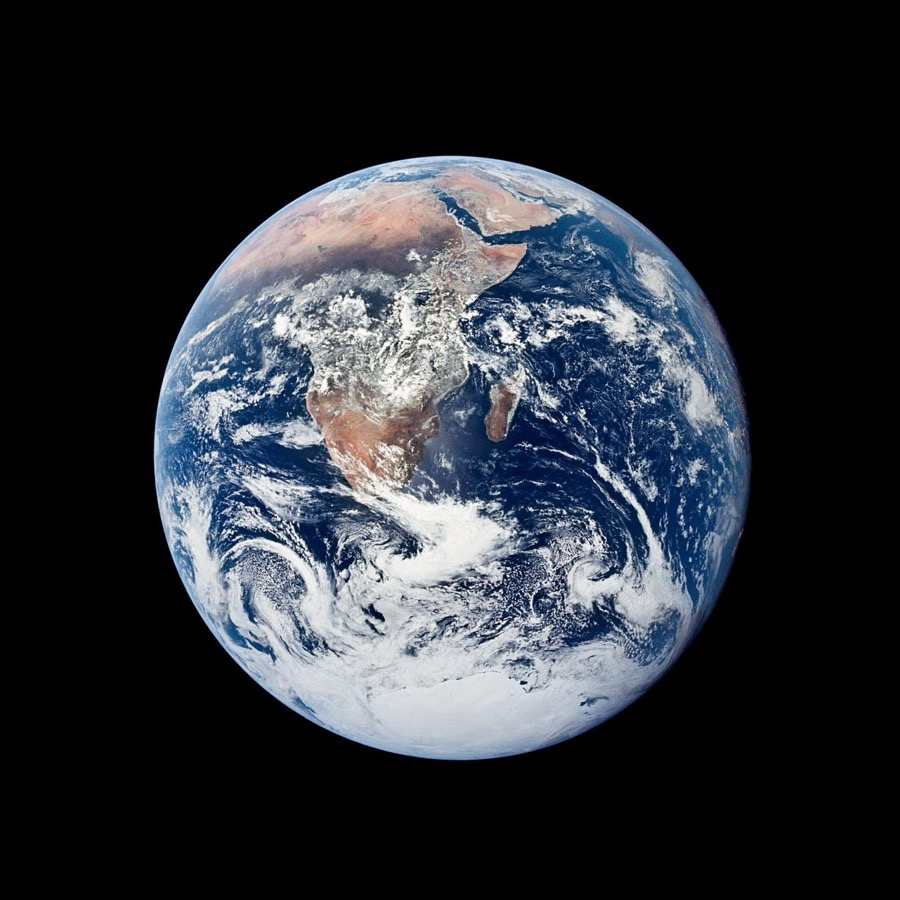
\includegraphics[width=0.55\linewidth]{images/blue-marble-nasa.jpg}
  \caption{Beispielabbildung mit Quellenangabe~\cite{nasa-blue-marble}}
  \label{abb:blue-marble}
\end{figure}

Vektorgrafiken haben gegenüber Screenshots den Vorteil, dass

\begin{itemize}
  \item sie jederzeit editiert werden können,
  \item sie beliebig skaliert werden können, ohne unscharf zu werden,
  \item alle Grafiken einheitlich vergrößert oder verkleinert werden können.
        Das verbessert das Layout ungemein.
\end{itemize}

Abbildungen stehen immer alleinstehend und zentriert. Die Breite wird
relativ zur Textbreite angegeben (\lstinline|width=0.75\linewidth|), damit
sie nie über den Satzspiegel hinausragt. Sollen mehrere Grafiken
nebeneinander stehen, verwendet dafür zwei \lstinline|minipage|-Umgebungen
innerhalb einer \lstinline|figure|.

Die Positionierung übernimmt \LaTeX. Die Angabe \lstinline|[htbp]| erlaubt
es, die Abbildung an die Stelle im Text, an den Seitenanfang, an das
Seitenende oder auf eine eigene Seite zu setzen. Eine Abbildung kann dadurch
auf der Folgeseite landen -- das ist beabsichtigt und kein Fehler.

\subsection{Beschriftungen}

Alle Grafiken und Tabellen sind zu beschriften und mit Quellenangaben zu
versehen. Im Text muss auf jede Abbildung und jede Tabelle Bezug genommen
werden.

Die Beschriftung erfolgt mit \lstinline|\caption| innerhalb der
\lstinline|figure|- bzw.\ \lstinline|table|-Umgebung. Nur so werden
Abbildungs- und Tabellenverzeichnis korrekt geführt. Bei Abbildungen steht
die Beschriftung unter der Grafik, bei Tabellen darüber; die Vorlage stellt
das automatisch richtig ein.

Abbildungen werden mit \enquote{Abb.} und Tabellen mit \enquote{Tab.}
bezeichnet. Auch das erledigt die Vorlage; die Nummerierung läuft
durchgehend und nicht kapitelweise. In englischsprachigen Diplomarbeiten
wird \enquote{Abb.} durch \enquote{Fig.} ersetzt -- dafür genügt die
Klassenoption \lstinline|englisch|.

Unmittelbar nach \lstinline|\caption| gehört ein \lstinline|\label|. Ohne
Label lässt sich die Abbildung später nicht referenzieren. Bewährt hat sich
ein Präfix je Objektart: \lstinline|abb:|, \lstinline|tab:| und
\lstinline|code:|.

\subsection{Querverweise}

Textpassagen, die sich auf andere Kapitel, Grafiken oder Tabellen beziehen,
müssen eine Referenz enthalten. Diese wird mit \lstinline|\ref| erzeugt und
enthält zumindest die Kategorie und die Nummer, also etwa
\lstinline|Abb.~\ref{abb:aufbau}|. Das geschützte Leerzeichen
\lstinline|~| verhindert, dass zwischen Bezeichnung und Nummer umgebrochen
wird.

Liegen referenzierender Text und referenziertes Objekt mehr als eine Seite
auseinander, ist zusätzlich die Seitenzahl mit \lstinline|\pageref|
anzugeben.

Anders als in Word müssen Querverweise und Verzeichnisse nicht manuell
aktualisiert werden. \LaTeX{} löst sie beim Übersetzen auf, benötigt dafür
aber mehrere Durchläufe. \lstinline|latexmk| (bzw.\ \lstinline|make pdf|)
wiederholt den Lauf so lange, bis sich nichts mehr ändert. Meldet das
Protokoll am Ende \enquote{There were undefined references}, fehlt ein
\lstinline|\label| oder es ist falsch geschrieben.

\subsection{Quellenangaben}

In wissenschaftlichen Arbeiten ist es verpflichtend, die Quelle jeder
Aussage anzugeben, die nicht von einem selbst stammt. Der Leser muss die
Möglichkeit haben, die Ausführungen des Autors nachzuprüfen.

Zu diesem Zweck müssen im Text der Diplomarbeit alle verwendeten Quellen
(Fachbücher, Fachzeitschriften, Herstellerunterlagen, Webseiten, \ldots)
angegeben werden. Dies geschieht am Ende des zitierten Textes durch Angabe
der Quelle. Informationen aus Lehrbüchern können als Allgemeinwissen
vorausgesetzt werden und müssen nicht zitiert werden.

Bei inhaltlichen Zitaten, dem Normalfall in technischen Arbeiten, wird der
Inhalt der Quelle nur sinngemäß wiedergegeben.

Bei wörtlichen Zitaten, die in technischen Arbeiten eher selten auftreten,
wird die wörtlich zitierte Textstelle zwischen Anführungszeichen gesetzt,
dahinter steht die Quellenangabe. Eigene Kommentare im Zitat oder
Verkürzungen werden in eckigen Klammern angegeben. Kurze Zitate stehen mit
\lstinline|\zitat| im Fließtext, längere in der Umgebung
\lstinline|zitatfreistehend|.

Beispiel für ein Zitat im Text der Diplomarbeit:
\zitat{[\ldots] kann in diesem Fall eine relationale Datenbank vorteilhaft
eingesetzt werden}~\cite{beispiel-buch}.

Beispiel für ein Zitat als eigener Absatz:

\begin{zitatfreistehend}
  \enquote{The basic guideline for citing online sources is to follow the
  standard citation for the citation, or add the DOI in place of page
  numbers if the source is not paginated.}~\cite{beispiel-artikel}
\end{zitatfreistehend}

Für Diplomarbeiten an der \ac{HTL} Donaustadt ist der IEEE-Zitierstil zu
verwenden. Jeder Quelle wird eine Nummer zugeordnet und in eckigen Klammern
angegeben. Diese Vorlage stellt den Stil bereits ein; zitiert wird mit
\lstinline|\cite{schluessel}|, wobei der Schlüssel aus
\lstinline|references.bib| stammt. Das Quellenverzeichnis wird daraus
automatisch erzeugt und enthält nur tatsächlich zitierte Einträge.

Zum Verwalten der Quellen empfiehlt sich Zotero mit dem Plug-in Better
BibTeX, das \lstinline|references.bib| bei jeder Änderung automatisch neu
exportiert.

Es gibt viele verschiedene Typen von Quellen. Tab.~\ref{tab:quellentypen}
zeigt die häufigsten, den passenden BibTeX-Eintragstyp und die
Informationen, die mindestens enthalten sein sollten.

\begin{table}[htbp]
  \centering
  \caption{Quellentypen}
  \label{tab:quellentypen}
  \begin{tabular}{@{}p{0.28\linewidth}p{0.16\linewidth}p{0.46\linewidth}@{}}
    \toprule
    \tabkopf{Quellentyp} & \tabkopf{Eintragstyp} &
      \tabkopf{wichtigste Informationen} \\
    \midrule
    Buch (auch E-Books, Broschüren) & \lstinline|@book| &
      Autor(en), Titel, Auflage, Verlag, Ort, ISBN \\
    Diplomarbeit, Dissertation & \lstinline|@thesis| &
      Autor(en), Titel, Institution, Ort, Datum \\
    Webseite (auch PDF) & \lstinline|@online| &
      Autor(en), Titel, URL, Abrufdatum (\lstinline|urldate|) \\
    Zeitschriftenartikel & \lstinline|@article| &
      Autor(en), Titel, Publikation, Band, Ausgabe, Seiten, Datum \\
    Verwendung von KI & \lstinline|@online| &
      siehe Anhang und die Vorgaben des Ministeriums~\cite{beispiel-online} \\
    \bottomrule
  \end{tabular}
\end{table}

\subsection{Befehle und Umgebungen}

In Word übernehmen Formatvorlagen das einheitliche Layout. In \LaTeX{}
erfüllen Befehle und Umgebungen dieselbe Aufgabe: Der Text beschreibt, was
etwas \emph{ist}, das Aussehen legt die Dokumentklasse \lstinline|htldon.cls|
zentral fest. Dadurch lässt sich die Formatierung nachträglich an einer
einzigen Stelle ändern.

Die in Tab.~\ref{tab:befehle} aufgeführten Befehle stellen sicher, dass alle
Diplomarbeiten den Richtlinien entsprechen. Sie dürfen nur in begründeten
Ausnahmefällen angepasst werden.

\begin{table}[htbp]
  \centering
  \caption{Befehle und Umgebungen der Vorlage}
  \label{tab:befehle}
  \begin{tabular}{@{}p{0.36\linewidth}p{0.58\linewidth}@{}}
    \toprule
    \tabkopf{Befehl} & \tabkopf{Beschreibung} \\
    \midrule
    \lstinline|\chapter| bis \lstinline|\subsubsection| &
      Kapitelüberschriften mit Dezimalklassifikation. Die ersten drei Ebenen
      erscheinen im Inhaltsverzeichnis, \lstinline|\subsubsection| nicht. \\
    \lstinline|\paragraph| &
      Zwischenüberschrift ohne Nummerierung, nicht im Inhaltsverzeichnis. \\
    \lstinline|\abschnittsautor| &
      Verfasser/in eines Abschnitts, erscheint rechts in der Kopfzeile.
      Format: erster Buchstabe des Vornamens, Punkt, Nachname
      (\enquote{M. Muster}). \\
    \lstinline|\zitat|, \lstinline|zitatfreistehend| &
      Kennzeichnung wörtlicher Zitate im Fließtext bzw.\ als eigener Absatz. \\
    \lstinline|\menue| &
      Menüstrukturen (\menue{Datei / Öffnen}) und Tastatureingaben
      (\menue{Strg + A}). \\
    \lstinline|lstlisting|, \lstinline|\lstinline| &
      Quellcode als eigener Block bzw.\ im Fließtext. \\
    \lstinline|\tabkopf| &
      Kopfzeile einer Tabelle. Der Tabelleninhalt selbst wird von der Klasse
      automatisch auf 10\,pt und linksbündig gestellt. \\
    \lstinline|\ac|, \lstinline|\acp| &
      Abkürzung, beim ersten Auftreten ausgeschrieben, im Plural mit
      \lstinline|\acp|. \\
    \lstinline|\cite|, \lstinline|\ref|, \lstinline|\pageref| &
      Quellenangabe, Querverweis, Seitenverweis. \\
    \bottomrule
  \end{tabular}
\end{table}

Überschriften der Kapitel müssen kurz, präzise und selbsterklärend sein.
Beispiele für unzureichende Überschriften: \enquote{5.3 Aufbau},
\enquote{5.3 Messergebnis}, \enquote{5.3 Beispiel}.

Bei Unterüberschriften gilt:

\begin{itemize}
  \item Es muss mindestens zwei Unterpunkte geben. Ein Abschnitt 3.2.1 darf
        daher nicht existieren, wenn kein 3.2.2 folgt.
  \item Unterpunkte sollten inhaltlich ausreichend gefüllt sein und
        mindestens eine halbe Seite umfassen.
  \item Unterpunkte, die lediglich aus einem einzelnen Satz bestehen, werden
        besser als Aufzählung dargestellt.
\end{itemize}

Für die Darstellung von Quellcode gilt:

\begin{itemize}
  \item Umfang:
        \begin{itemize}
          \item Der vollständige Sourcecode gehört ausschließlich auf das
                elektronische Speichermedium.
          \item Im Dokument selbst sollen nur wesentliche Ausschnitte
                aufgenommen werden.
        \end{itemize}
  \item Formatierung: Schriftart und Schriftgröße gibt die
        \lstinline|lstlisting|-Umgebung vor, der Zeilenabstand ist dort
        einzeilig. Die Sprache wird mit
        \lstinline|[language=Python]| angegeben, damit die
        Syntaxhervorhebung stimmt.
  \item Inhaltliche Anforderungen: Der Sourcecode muss ausreichend
        kommentiert sein.
  \item Verwendung im Fließtext: Wird Sourcecode im Text erwähnt, ist
        \lstinline|\lstinline| zu verwenden. Zusätzliche Anführungszeichen
        sind nicht erforderlich. Beispiel: Mit dem Befehl
        \lstinline|ShowModal| wird ein Frame geöffnet.
\end{itemize}

\section{Beschreibung der Kapitel}

\subsection{Titelseite}

Die Titelseite wird vollständig aus \lstinline|metadata.tex| erzeugt. Dort
sind einzutragen:

\begin{itemize}
  \item der Titel der Diplomarbeit mit \lstinline|\titel|. Er wird
        automatisch in die Kopfzeile übernommen.
  \item ein Projektlogo, Bild oder eine Zeichnung mit
        \lstinline|\projektlogo|.
  \item alle Verfasser/innen mit \lstinline|\teammitglied| und die
        Betreuung mit \lstinline|\betreuung|.
  \item Schuljahr, Abteilung und Klasse.
\end{itemize}

Falls alle Verfasser/innen oder Betreuer/innen dasselbe Geschlecht haben,
kann die geschlechtsspezifische Form verwendet werden; dafür ist das
optionale Argument von \lstinline|\betreuung| vorgesehen.

\subsection{Verfassererklärung}

In der Verfassererklärung bekennen sich die Verfasser/innen zu einem
wissenschaftlichen Arbeitsstil. Sollten im Nachhinein grobe Verstöße dagegen
aufgedeckt werden, kann die Arbeit für ungültig erklärt und der Abschluss
revidiert werden.

Die Erklärung erzeugt \lstinline|\eigenstaendigkeitserklaerung|. Je
Teammitglied entsteht automatisch eine Unterschriftszeile. Zu ergänzen sind
gegebenenfalls Kooperationen mit Firmen und Sperrvermerke.

\subsection{Problemstellung}

Die Seite \enquote{Problemstellung} wird durch den eingescannten Antrag (mit
allen Stempeln und Unterschriften) vollflächig ersetzt. Dazu wird in
\lstinline|frontmatter/problem-statement.tex| das Scan-PDF eingebunden.

\subsection{Kurzfassung bzw.\ Abstract}

Die Kurzfassung bzw.\ der Abstract soll kurz, prägnant und verständlich den
Inhalt der Arbeit wiedergeben: Zielsetzung, Ablauf, wichtigste Erkenntnisse,
wesentliche Merkmale des realisierten Produkts, Schlussfolgerungen und
Ausblick. Beide sind als eigenständiges Dokument zu konzipieren, das
unabhängig von der Diplomarbeit gelesen und verstanden werden kann, und
sollen in Deutsch und Englisch jeweils nicht mehr als eine Seite umfassen.

\subsection{Inhaltsverzeichnis}

Das Inhaltsverzeichnis wird automatisch aus den Überschriften erstellt. Es
zeigt die ersten drei Ebenen, der Text steht linksbündig, die Seitenzahlen
rechtsbündig, als Füllzeichen dienen Punkte. Eine manuelle Aktualisierung
ist nicht nötig.

\subsection{Die weiteren Kapitel}

Die Kapitel Projektplanung, Technische Grundlagen, Praktische Realisierung
sowie Evaluierung und Ergebnisse beschreiben die Diplomarbeit im Detail.

Für die Beurteilung ist es wichtig, den/die Verfasser/in zu kennen. Daher
ist dieser Hinweis auf jeder Seite rechtsbündig in der Kopfzeile zu
vermerken. Dafür wird \lstinline|\abschnittsautor| direkt nach der
Überschrift gesetzt; der Eintrag gilt ab dort bis zur nächsten Angabe.
Haben mehrere Personen gemeinsam an einem Abschnitt gearbeitet, sind alle zu
nennen, durch Komma getrennt:
\lstinline|\abschnittsautor{A. Erste, B. Zweite}|.

Die Projektplanung soll die systematische Durchführung der Diplomarbeit
innerhalb des Projektteams beschreiben. Dabei sollen geplante Ziele und
tatsächlich erreichte Ergebnisse miteinander verglichen und die Unterschiede
reflektiert werden. Beim klassischen Wasserfall-Projektmanagement können
etwa die Meilensteine als Referenz dienen, bei agiler Projektorganisation
die Sprint-Reviews.

Im Kapitel Technische Grundlagen finden sich alle für das unmittelbare
technische Verständnis der Diplomarbeit relevanten Inhalte. Hier wird
insbesondere auf korrekte Zitate und den sorgfältigen Einsatz von Quellen
geachtet.

Das Kapitel Praktische Realisierung enthält die praktischen Eigenleistungen
der Diplomarbeit. Dabei sollen die Vorgänge und Untersuchungen beschrieben
und nachvollziehbar dokumentiert werden.

Im Kapitel Evaluierung und Ergebnisse erfolgt die Darstellung und Bewertung
der abschließenden Arbeit. Hier soll ebenso, sofern vorhanden, das
Endprodukt bzw.\ der Prototyp präsentiert und beschrieben werden.

\subsection{Anhang}

Im Anhang können alle Informationen gesammelt werden, die zwar zur
Diplomarbeit gehören, jedoch im Inhaltsteil den Rahmen gesprengt hätten.
Dazu zählen wichtige Notizen (z.\,B. Gesprächsprotokolle), Normen,
Schnittstellendefinitionen oder Präsentationen. Weiters soll der Anhang den
Inhalt eines beigefügten elektronischen Speichermediums sowie einen
einseitigen Lebenslauf jedes Teammitglieds enthalten.

Verpflichtend ist außerdem die Dokumentation aller eingesetzten KI-basierten
Hilfsmittel. Dafür ist \lstinline|appendix/ai-tools.tex| vorgesehen.
| zu löschen. Die Einträge
im Inhaltsverzeichnis und in den übrigen Verzeichnissen verschwinden beim
nächsten Übersetzen von selbst.

\subsection{Abgabe der Diplomarbeit}

Die Diplomarbeit ist in gedruckter bzw.\ gebundener Form und in digitaler
Form vorzulegen. Dem Abteilungsvorstand sind zwei geheftete Exemplare (ein
Belegexemplar und ein Beurteilungsexemplar für den/die Betreuer/in) zu
übergeben.

Nach erfolgter Beurteilung geht das Beurteilungsexemplar temporär zurück an
die Diplomarbeitsgruppe. Nun können letzte Korrekturen (ohne
Beurteilungsrelevanz) vorgenommen werden. Anschließend wird die Arbeit erneut
ausgedruckt und gesammelt zur Bindung außer Haus gegeben. Weitere Exemplare
für Kooperationspartner (Firmen, Institutionen) oder Projektteilnehmer können
in diesem Zusammenhang erstellt werden.

\subsection{Grafiken}

Abbildungen müssen in gut lesbarer Bildqualität eingefügt werden. Grafiken
sollten am besten in einem vektorbasierten Zeichenprogramm (z.\,B. Inkscape,
draw.io) erstellt und als PDF exportiert werden; PDF und PNG lassen sich
direkt einbinden, SVG nicht. Alle Bilddateien gehören in den Ordner
\lstinline|images/|.

\begin{lstlisting}[language={[LaTeX]TeX}, caption={Eine Abbildung einbinden},
                   label=code:abbildung]
\begin{figure}[htbp]
  \centering
  
\includegraphics[width=0.75\linewidth]{images/example-figure.pdf}
  \caption{Aufbau des Systems}
  \label{abb:aufbau}
\end{figure}
\end{lstlisting}

Abb.~\ref{abb:blue-marble} zeigt, wie das Ergebnis aussieht. Stammt die
Grafik nicht von euch selbst, gehört die Quelle in die Beschriftung.

\begin{figure}[htbp]
  \centering
  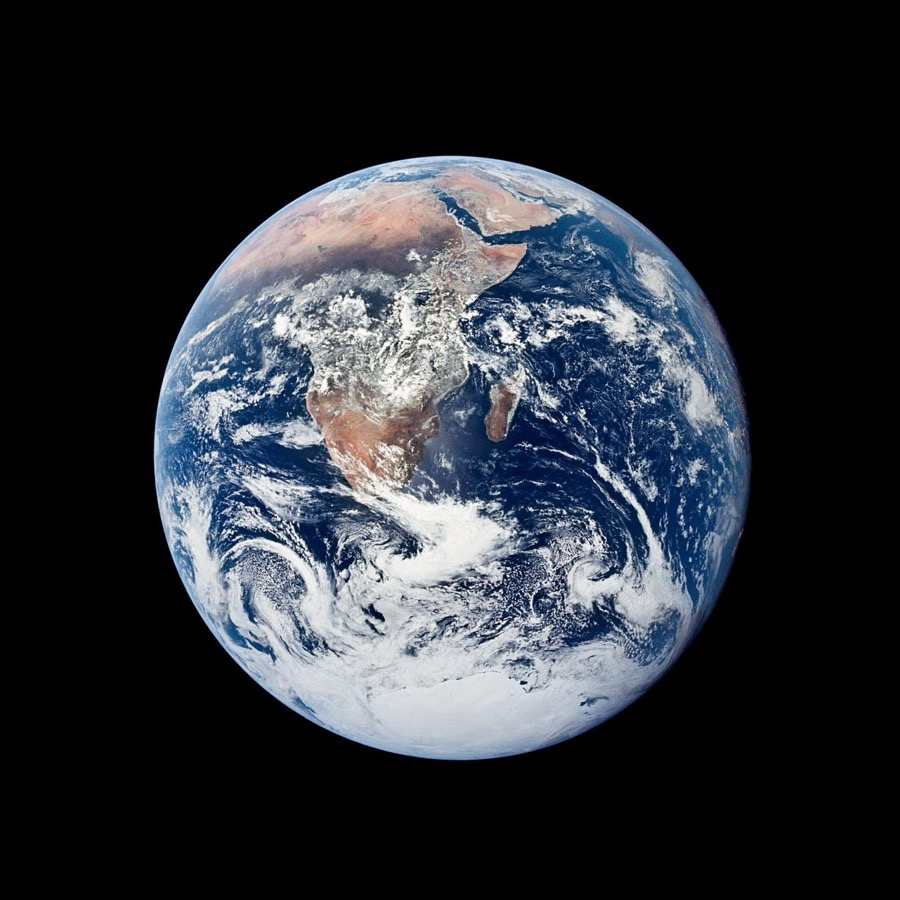
\includegraphics[width=0.55\linewidth]{images/blue-marble-nasa.jpg}
  \caption{Beispielabbildung mit Quellenangabe~\cite{nasa-blue-marble}}
  \label{abb:blue-marble}
\end{figure}

Vektorgrafiken haben gegenüber Screenshots den Vorteil, dass

\begin{itemize}
  \item sie jederzeit editiert werden können,
  \item sie beliebig skaliert werden können, ohne unscharf zu werden,
  \item alle Grafiken einheitlich vergrößert oder verkleinert werden können.
        Das verbessert das Layout ungemein.
\end{itemize}

Abbildungen stehen immer alleinstehend und zentriert. Die Breite wird
relativ zur Textbreite angegeben (\lstinline|width=0.75\linewidth|), damit
sie nie über den Satzspiegel hinausragt. Sollen mehrere Grafiken
nebeneinander stehen, verwendet dafür zwei \lstinline|minipage|-Umgebungen
innerhalb einer \lstinline|figure|.

Die Positionierung übernimmt \LaTeX. Die Angabe \lstinline|[htbp]| erlaubt
es, die Abbildung an die Stelle im Text, an den Seitenanfang, an das
Seitenende oder auf eine eigene Seite zu setzen. Eine Abbildung kann dadurch
auf der Folgeseite landen -- das ist beabsichtigt und kein Fehler.

\subsection{Beschriftungen}

Alle Grafiken und Tabellen sind zu beschriften und mit Quellenangaben zu
versehen. Im Text muss auf jede Abbildung und jede Tabelle Bezug genommen
werden.

Die Beschriftung erfolgt mit \lstinline|\caption| innerhalb der
\lstinline|figure|- bzw.\ \lstinline|table|-Umgebung. Nur so werden
Abbildungs- und Tabellenverzeichnis korrekt geführt. Bei Abbildungen steht
die Beschriftung unter der Grafik, bei Tabellen darüber; die Vorlage stellt
das automatisch richtig ein.

Abbildungen werden mit \enquote{Abb.} und Tabellen mit \enquote{Tab.}
bezeichnet. Auch das erledigt die Vorlage; die Nummerierung läuft
durchgehend und nicht kapitelweise. In englischsprachigen Diplomarbeiten
wird \enquote{Abb.} durch \enquote{Fig.} ersetzt -- dafür genügt die
Klassenoption \lstinline|englisch|.

Unmittelbar nach \lstinline|\caption| gehört ein \lstinline|\label|. Ohne
Label lässt sich die Abbildung später nicht referenzieren. Bewährt hat sich
ein Präfix je Objektart: \lstinline|abb:|, \lstinline|tab:| und
\lstinline|code:|.

\subsection{Querverweise}

Textpassagen, die sich auf andere Kapitel, Grafiken oder Tabellen beziehen,
müssen eine Referenz enthalten. Diese wird mit \lstinline|\ref| erzeugt und
enthält zumindest die Kategorie und die Nummer, also etwa
\lstinline|Abb.~\ref{abb:aufbau}|. Das geschützte Leerzeichen
\lstinline|~| verhindert, dass zwischen Bezeichnung und Nummer umgebrochen
wird.

Liegen referenzierender Text und referenziertes Objekt mehr als eine Seite
auseinander, ist zusätzlich die Seitenzahl mit \lstinline|\pageref|
anzugeben.

Anders als in Word müssen Querverweise und Verzeichnisse nicht manuell
aktualisiert werden. \LaTeX{} löst sie beim Übersetzen auf, benötigt dafür
aber mehrere Durchläufe. \lstinline|latexmk| (bzw.\ \lstinline|make pdf|)
wiederholt den Lauf so lange, bis sich nichts mehr ändert. Meldet das
Protokoll am Ende \enquote{There were undefined references}, fehlt ein
\lstinline|\label| oder es ist falsch geschrieben.

\subsection{Quellenangaben}

In wissenschaftlichen Arbeiten ist es verpflichtend, die Quelle jeder
Aussage anzugeben, die nicht von einem selbst stammt. Der Leser muss die
Möglichkeit haben, die Ausführungen des Autors nachzuprüfen.

Zu diesem Zweck müssen im Text der Diplomarbeit alle verwendeten Quellen
(Fachbücher, Fachzeitschriften, Herstellerunterlagen, Webseiten, \ldots)
angegeben werden. Dies geschieht am Ende des zitierten Textes durch Angabe
der Quelle. Informationen aus Lehrbüchern können als Allgemeinwissen
vorausgesetzt werden und müssen nicht zitiert werden.

Bei inhaltlichen Zitaten, dem Normalfall in technischen Arbeiten, wird der
Inhalt der Quelle nur sinngemäß wiedergegeben.

Bei wörtlichen Zitaten, die in technischen Arbeiten eher selten auftreten,
wird die wörtlich zitierte Textstelle zwischen Anführungszeichen gesetzt,
dahinter steht die Quellenangabe. Eigene Kommentare im Zitat oder
Verkürzungen werden in eckigen Klammern angegeben. Kurze Zitate stehen mit
\lstinline|\zitat| im Fließtext, längere in der Umgebung
\lstinline|zitatfreistehend|.

Beispiel für ein Zitat im Text der Diplomarbeit:
\zitat{[\ldots] kann in diesem Fall eine relationale Datenbank vorteilhaft
eingesetzt werden}~\cite{beispiel-buch}.

Beispiel für ein Zitat als eigener Absatz:

\begin{zitatfreistehend}
  \enquote{The basic guideline for citing online sources is to follow the
  standard citation for the citation, or add the DOI in place of page
  numbers if the source is not paginated.}~\cite{beispiel-artikel}
\end{zitatfreistehend}

Für Diplomarbeiten an der \ac{HTL} Donaustadt ist der IEEE-Zitierstil zu
verwenden. Jeder Quelle wird eine Nummer zugeordnet und in eckigen Klammern
angegeben. Diese Vorlage stellt den Stil bereits ein; zitiert wird mit
\lstinline|\cite{schluessel}|, wobei der Schlüssel aus
\lstinline|references.bib| stammt. Das Quellenverzeichnis wird daraus
automatisch erzeugt und enthält nur tatsächlich zitierte Einträge.

Zum Verwalten der Quellen empfiehlt sich Zotero mit dem Plug-in Better
BibTeX, das \lstinline|references.bib| bei jeder Änderung automatisch neu
exportiert.

Es gibt viele verschiedene Typen von Quellen. Tab.~\ref{tab:quellentypen}
zeigt die häufigsten, den passenden BibTeX-Eintragstyp und die
Informationen, die mindestens enthalten sein sollten.

\begin{table}[htbp]
  \centering
  \caption{Quellentypen}
  \label{tab:quellentypen}
  \begin{tabular}{@{}p{0.28\linewidth}p{0.16\linewidth}p{0.46\linewidth}@{}}
    \toprule
    \tabkopf{Quellentyp} & \tabkopf{Eintragstyp} &
      \tabkopf{wichtigste Informationen} \\
    \midrule
    Buch (auch E-Books, Broschüren) & \lstinline|@book| &
      Autor(en), Titel, Auflage, Verlag, Ort, ISBN \\
    Diplomarbeit, Dissertation & \lstinline|@thesis| &
      Autor(en), Titel, Institution, Ort, Datum \\
    Webseite (auch PDF) & \lstinline|@online| &
      Autor(en), Titel, URL, Abrufdatum (\lstinline|urldate|) \\
    Zeitschriftenartikel & \lstinline|@article| &
      Autor(en), Titel, Publikation, Band, Ausgabe, Seiten, Datum \\
    Verwendung von KI & \lstinline|@online| &
      siehe Anhang und die Vorgaben des Ministeriums~\cite{beispiel-online} \\
    \bottomrule
  \end{tabular}
\end{table}

\subsection{Befehle und Umgebungen}

In Word übernehmen Formatvorlagen das einheitliche Layout. In \LaTeX{}
erfüllen Befehle und Umgebungen dieselbe Aufgabe: Der Text beschreibt, was
etwas \emph{ist}, das Aussehen legt die Dokumentklasse \lstinline|htldon.cls|
zentral fest. Dadurch lässt sich die Formatierung nachträglich an einer
einzigen Stelle ändern.

Die in Tab.~\ref{tab:befehle} aufgeführten Befehle stellen sicher, dass alle
Diplomarbeiten den Richtlinien entsprechen. Sie dürfen nur in begründeten
Ausnahmefällen angepasst werden.

\begin{table}[htbp]
  \centering
  \caption{Befehle und Umgebungen der Vorlage}
  \label{tab:befehle}
  \begin{tabular}{@{}p{0.36\linewidth}p{0.58\linewidth}@{}}
    \toprule
    \tabkopf{Befehl} & \tabkopf{Beschreibung} \\
    \midrule
    \lstinline|\chapter| bis \lstinline|\subsubsection| &
      Kapitelüberschriften mit Dezimalklassifikation. Die ersten drei Ebenen
      erscheinen im Inhaltsverzeichnis, \lstinline|\subsubsection| nicht. \\
    \lstinline|\paragraph| &
      Zwischenüberschrift ohne Nummerierung, nicht im Inhaltsverzeichnis. \\
    \lstinline|\abschnittsautor| &
      Verfasser/in eines Abschnitts, erscheint rechts in der Kopfzeile.
      Format: erster Buchstabe des Vornamens, Punkt, Nachname
      (\enquote{M. Muster}). \\
    \lstinline|\zitat|, \lstinline|zitatfreistehend| &
      Kennzeichnung wörtlicher Zitate im Fließtext bzw.\ als eigener Absatz. \\
    \lstinline|\menue| &
      Menüstrukturen (\menue{Datei / Öffnen}) und Tastatureingaben
      (\menue{Strg + A}). \\
    \lstinline|lstlisting|, \lstinline|\lstinline| &
      Quellcode als eigener Block bzw.\ im Fließtext. \\
    \lstinline|\tabkopf| &
      Kopfzeile einer Tabelle. Der Tabelleninhalt selbst wird von der Klasse
      automatisch auf 10\,pt und linksbündig gestellt. \\
    \lstinline|\ac|, \lstinline|\acp| &
      Abkürzung, beim ersten Auftreten ausgeschrieben, im Plural mit
      \lstinline|\acp|. \\
    \lstinline|\cite|, \lstinline|\ref|, \lstinline|\pageref| &
      Quellenangabe, Querverweis, Seitenverweis. \\
    \bottomrule
  \end{tabular}
\end{table}

Überschriften der Kapitel müssen kurz, präzise und selbsterklärend sein.
Beispiele für unzureichende Überschriften: \enquote{5.3 Aufbau},
\enquote{5.3 Messergebnis}, \enquote{5.3 Beispiel}.

Bei Unterüberschriften gilt:

\begin{itemize}
  \item Es muss mindestens zwei Unterpunkte geben. Ein Abschnitt 3.2.1 darf
        daher nicht existieren, wenn kein 3.2.2 folgt.
  \item Unterpunkte sollten inhaltlich ausreichend gefüllt sein und
        mindestens eine halbe Seite umfassen.
  \item Unterpunkte, die lediglich aus einem einzelnen Satz bestehen, werden
        besser als Aufzählung dargestellt.
\end{itemize}

Für die Darstellung von Quellcode gilt:

\begin{itemize}
  \item Umfang:
        \begin{itemize}
          \item Der vollständige Sourcecode gehört ausschließlich auf das
                elektronische Speichermedium.
          \item Im Dokument selbst sollen nur wesentliche Ausschnitte
                aufgenommen werden.
        \end{itemize}
  \item Formatierung: Schriftart und Schriftgröße gibt die
        \lstinline|lstlisting|-Umgebung vor, der Zeilenabstand ist dort
        einzeilig. Die Sprache wird mit
        \lstinline|[language=Python]| angegeben, damit die
        Syntaxhervorhebung stimmt.
  \item Inhaltliche Anforderungen: Der Sourcecode muss ausreichend
        kommentiert sein.
  \item Verwendung im Fließtext: Wird Sourcecode im Text erwähnt, ist
        \lstinline|\lstinline| zu verwenden. Zusätzliche Anführungszeichen
        sind nicht erforderlich. Beispiel: Mit dem Befehl
        \lstinline|ShowModal| wird ein Frame geöffnet.
\end{itemize}

\section{Beschreibung der Kapitel}

\subsection{Titelseite}

Die Titelseite wird vollständig aus \lstinline|metadata.tex| erzeugt. Dort
sind einzutragen:

\begin{itemize}
  \item der Titel der Diplomarbeit mit \lstinline|\titel|. Er wird
        automatisch in die Kopfzeile übernommen.
  \item ein Projektlogo, Bild oder eine Zeichnung mit
        \lstinline|\projektlogo|.
  \item alle Verfasser/innen mit \lstinline|\teammitglied| und die
        Betreuung mit \lstinline|\betreuung|.
  \item Schuljahr, Abteilung und Klasse.
\end{itemize}

Falls alle Verfasser/innen oder Betreuer/innen dasselbe Geschlecht haben,
kann die geschlechtsspezifische Form verwendet werden; dafür ist das
optionale Argument von \lstinline|\betreuung| vorgesehen.

\subsection{Verfassererklärung}

In der Verfassererklärung bekennen sich die Verfasser/innen zu einem
wissenschaftlichen Arbeitsstil. Sollten im Nachhinein grobe Verstöße dagegen
aufgedeckt werden, kann die Arbeit für ungültig erklärt und der Abschluss
revidiert werden.

Die Erklärung erzeugt \lstinline|\eigenstaendigkeitserklaerung|. Je
Teammitglied entsteht automatisch eine Unterschriftszeile. Zu ergänzen sind
gegebenenfalls Kooperationen mit Firmen und Sperrvermerke.

\subsection{Problemstellung}

Die Seite \enquote{Problemstellung} wird durch den eingescannten Antrag (mit
allen Stempeln und Unterschriften) vollflächig ersetzt. Dazu wird in
\lstinline|frontmatter/problem-statement.tex| das Scan-PDF eingebunden.

\subsection{Kurzfassung bzw.\ Abstract}

Die Kurzfassung bzw.\ der Abstract soll kurz, prägnant und verständlich den
Inhalt der Arbeit wiedergeben: Zielsetzung, Ablauf, wichtigste Erkenntnisse,
wesentliche Merkmale des realisierten Produkts, Schlussfolgerungen und
Ausblick. Beide sind als eigenständiges Dokument zu konzipieren, das
unabhängig von der Diplomarbeit gelesen und verstanden werden kann, und
sollen in Deutsch und Englisch jeweils nicht mehr als eine Seite umfassen.

\subsection{Inhaltsverzeichnis}

Das Inhaltsverzeichnis wird automatisch aus den Überschriften erstellt. Es
zeigt die ersten drei Ebenen, der Text steht linksbündig, die Seitenzahlen
rechtsbündig, als Füllzeichen dienen Punkte. Eine manuelle Aktualisierung
ist nicht nötig.

\subsection{Die weiteren Kapitel}

Die Kapitel Projektplanung, Technische Grundlagen, Praktische Realisierung
sowie Evaluierung und Ergebnisse beschreiben die Diplomarbeit im Detail.

Für die Beurteilung ist es wichtig, den/die Verfasser/in zu kennen. Daher
ist dieser Hinweis auf jeder Seite rechtsbündig in der Kopfzeile zu
vermerken. Dafür wird \lstinline|\abschnittsautor| direkt nach der
Überschrift gesetzt; der Eintrag gilt ab dort bis zur nächsten Angabe.
Haben mehrere Personen gemeinsam an einem Abschnitt gearbeitet, sind alle zu
nennen, durch Komma getrennt:
\lstinline|\abschnittsautor{A. Erste, B. Zweite}|.

Die Projektplanung soll die systematische Durchführung der Diplomarbeit
innerhalb des Projektteams beschreiben. Dabei sollen geplante Ziele und
tatsächlich erreichte Ergebnisse miteinander verglichen und die Unterschiede
reflektiert werden. Beim klassischen Wasserfall-Projektmanagement können
etwa die Meilensteine als Referenz dienen, bei agiler Projektorganisation
die Sprint-Reviews.

Im Kapitel Technische Grundlagen finden sich alle für das unmittelbare
technische Verständnis der Diplomarbeit relevanten Inhalte. Hier wird
insbesondere auf korrekte Zitate und den sorgfältigen Einsatz von Quellen
geachtet.

Das Kapitel Praktische Realisierung enthält die praktischen Eigenleistungen
der Diplomarbeit. Dabei sollen die Vorgänge und Untersuchungen beschrieben
und nachvollziehbar dokumentiert werden.

Im Kapitel Evaluierung und Ergebnisse erfolgt die Darstellung und Bewertung
der abschließenden Arbeit. Hier soll ebenso, sofern vorhanden, das
Endprodukt bzw.\ der Prototyp präsentiert und beschrieben werden.

\subsection{Anhang}

Im Anhang können alle Informationen gesammelt werden, die zwar zur
Diplomarbeit gehören, jedoch im Inhaltsteil den Rahmen gesprengt hätten.
Dazu zählen wichtige Notizen (z.\,B. Gesprächsprotokolle), Normen,
Schnittstellendefinitionen oder Präsentationen. Weiters soll der Anhang den
Inhalt eines beigefügten elektronischen Speichermediums sowie einen
einseitigen Lebenslauf jedes Teammitglieds enthalten.

Verpflichtend ist außerdem die Dokumentation aller eingesetzten KI-basierten
Hilfsmittel. Dafür ist \lstinline|appendix/ai-tools.tex| vorgesehen.

% in diplomarbeit.tex entfernen und diese Datei mitlöschen.
% =====================================================================
\chapter{Richtlinie für das Verfassen von Diplomarbeiten}

Diese Richtlinie beschreibt die formalen und inhaltlichen Anforderungen an
eine wissenschaftliche Publikation und soll ein einheitliches
Erscheinungsbild der Diplomarbeiten sicherstellen. Dieses Kapitel beschreibt
weiters, wie die vorliegende Diplomarbeitsvorlage zu verwenden ist, und ist
im finalen Dokument zu entfernen.

Es sind bewusst nur die wesentlichen Punkte festgelegt. In Absprache mit dem
Betreuer/der Betreuerin soll stets Freiraum für die individuelle Gestaltung
sowie projektbedingte Erfordernisse bleiben.

\section{Allgemein}

Die Diplomarbeit soll kurz und prägnant -- aber vollständig -- gehalten sein
und einen Umfang von ca.\ 70 Seiten (ohne Anhang) bei einer Teamgröße von
2 Personen umfassen. Die inhaltliche Qualität bei in Umfang eingeschränkter
Darstellung ist ein wesentliches Ziel jeder wissenschaftlichen Publikation
und wird auch in die Beurteilung einbezogen. Grafische Darstellungen,
Übersichtstabellen und Diagramme sind wichtige Hilfsmittel, um diese Vorgabe
einhalten zu können.

Einige Tipps:

\begin{itemize}
  \item Das Verwenden der \enquote{ich}- und \enquote{wir}-Form sowie von
        \enquote{man}-Aussagen ist zu vermeiden.
  \item Abkürzungen müssen unmittelbar nach ihrem ersten Auftreten erläutert
        werden; falls erforderlich, ist ein Abkürzungsverzeichnis zu
        erstellen. Der Befehl \lstinline|\ac{API}| erledigt das automatisch:
        beim ersten Auftreten schreibt er die Abkürzung aus, danach nicht
        mehr.
  \item Über Themen, die nur indirekt mit der gestellten Aufgabe zu tun
        haben, soll nicht berichtet werden. Die ausführliche Darstellung von
        Grundlagenwissen ist nicht erforderlich; meistens reicht das Zitieren
        geeigneter Quellen.
  \item Arbeitet im Team über ein Git-Repository und legt pro Kapitel eine
        eigene Datei an. So lassen sich Änderungen nachvollziehen und
        Konflikte auf einzelne Absätze eingrenzen.
\end{itemize}

\subsection{Platzhalter in dieser Vorlage}

Alle Beispieltexte in dieser Vorlage sind zu ersetzen oder zu löschen. Das
betrifft insbesondere:

\begin{itemize}
  \item die Metadaten in \lstinline|metadata.tex| (Titel, Team, Betreuung,
        Schuljahr, Klasse),
  \item die Beispielkapitel in \lstinline|chapters/|,
  \item die Beispielquellen in \lstinline|references.bib|,
  \item das Abkürzungsverzeichnis in \lstinline|diplomarbeit.tex|,
  \item dieses gesamte Kapitel~6.
\end{itemize}

Um dieses Kapitel zu entfernen, genügt es, in \lstinline|diplomarbeit.tex|
die Zeile \lstinline|% =====================================================================
% Kapitel 6 der Abteilungsvorlage, auf LaTeX übertragen.
% Vor der Abgabe komplett löschen: die Zeile % =====================================================================
% Kapitel 6 der Abteilungsvorlage, auf LaTeX übertragen.
% Vor der Abgabe komplett löschen: die Zeile \input{chapters/06-guideline}
% in diplomarbeit.tex entfernen und diese Datei mitlöschen.
% =====================================================================
\chapter{Richtlinie für das Verfassen von Diplomarbeiten}

Diese Richtlinie beschreibt die formalen und inhaltlichen Anforderungen an
eine wissenschaftliche Publikation und soll ein einheitliches
Erscheinungsbild der Diplomarbeiten sicherstellen. Dieses Kapitel beschreibt
weiters, wie die vorliegende Diplomarbeitsvorlage zu verwenden ist, und ist
im finalen Dokument zu entfernen.

Es sind bewusst nur die wesentlichen Punkte festgelegt. In Absprache mit dem
Betreuer/der Betreuerin soll stets Freiraum für die individuelle Gestaltung
sowie projektbedingte Erfordernisse bleiben.

\section{Allgemein}

Die Diplomarbeit soll kurz und prägnant -- aber vollständig -- gehalten sein
und einen Umfang von ca.\ 70 Seiten (ohne Anhang) bei einer Teamgröße von
2 Personen umfassen. Die inhaltliche Qualität bei in Umfang eingeschränkter
Darstellung ist ein wesentliches Ziel jeder wissenschaftlichen Publikation
und wird auch in die Beurteilung einbezogen. Grafische Darstellungen,
Übersichtstabellen und Diagramme sind wichtige Hilfsmittel, um diese Vorgabe
einhalten zu können.

Einige Tipps:

\begin{itemize}
  \item Das Verwenden der \enquote{ich}- und \enquote{wir}-Form sowie von
        \enquote{man}-Aussagen ist zu vermeiden.
  \item Abkürzungen müssen unmittelbar nach ihrem ersten Auftreten erläutert
        werden; falls erforderlich, ist ein Abkürzungsverzeichnis zu
        erstellen. Der Befehl \lstinline|\ac{API}| erledigt das automatisch:
        beim ersten Auftreten schreibt er die Abkürzung aus, danach nicht
        mehr.
  \item Über Themen, die nur indirekt mit der gestellten Aufgabe zu tun
        haben, soll nicht berichtet werden. Die ausführliche Darstellung von
        Grundlagenwissen ist nicht erforderlich; meistens reicht das Zitieren
        geeigneter Quellen.
  \item Arbeitet im Team über ein Git-Repository und legt pro Kapitel eine
        eigene Datei an. So lassen sich Änderungen nachvollziehen und
        Konflikte auf einzelne Absätze eingrenzen.
\end{itemize}

\subsection{Platzhalter in dieser Vorlage}

Alle Beispieltexte in dieser Vorlage sind zu ersetzen oder zu löschen. Das
betrifft insbesondere:

\begin{itemize}
  \item die Metadaten in \lstinline|metadata.tex| (Titel, Team, Betreuung,
        Schuljahr, Klasse),
  \item die Beispielkapitel in \lstinline|chapters/|,
  \item die Beispielquellen in \lstinline|references.bib|,
  \item das Abkürzungsverzeichnis in \lstinline|diplomarbeit.tex|,
  \item dieses gesamte Kapitel~6.
\end{itemize}

Um dieses Kapitel zu entfernen, genügt es, in \lstinline|diplomarbeit.tex|
die Zeile \lstinline|\input{chapters/06-guideline}| zu löschen. Die Einträge
im Inhaltsverzeichnis und in den übrigen Verzeichnissen verschwinden beim
nächsten Übersetzen von selbst.

\subsection{Abgabe der Diplomarbeit}

Die Diplomarbeit ist in gedruckter bzw.\ gebundener Form und in digitaler
Form vorzulegen. Dem Abteilungsvorstand sind zwei geheftete Exemplare (ein
Belegexemplar und ein Beurteilungsexemplar für den/die Betreuer/in) zu
übergeben.

Nach erfolgter Beurteilung geht das Beurteilungsexemplar temporär zurück an
die Diplomarbeitsgruppe. Nun können letzte Korrekturen (ohne
Beurteilungsrelevanz) vorgenommen werden. Anschließend wird die Arbeit erneut
ausgedruckt und gesammelt zur Bindung außer Haus gegeben. Weitere Exemplare
für Kooperationspartner (Firmen, Institutionen) oder Projektteilnehmer können
in diesem Zusammenhang erstellt werden.

\subsection{Grafiken}

Abbildungen müssen in gut lesbarer Bildqualität eingefügt werden. Grafiken
sollten am besten in einem vektorbasierten Zeichenprogramm (z.\,B. Inkscape,
draw.io) erstellt und als PDF exportiert werden; PDF und PNG lassen sich
direkt einbinden, SVG nicht. Alle Bilddateien gehören in den Ordner
\lstinline|images/|.

\begin{lstlisting}[language={[LaTeX]TeX}, caption={Eine Abbildung einbinden},
                   label=code:abbildung]
\begin{figure}[htbp]
  \centering
  
\includegraphics[width=0.75\linewidth]{images/example-figure.pdf}
  \caption{Aufbau des Systems}
  \label{abb:aufbau}
\end{figure}
\end{lstlisting}

Abb.~\ref{abb:blue-marble} zeigt, wie das Ergebnis aussieht. Stammt die
Grafik nicht von euch selbst, gehört die Quelle in die Beschriftung.

\begin{figure}[htbp]
  \centering
  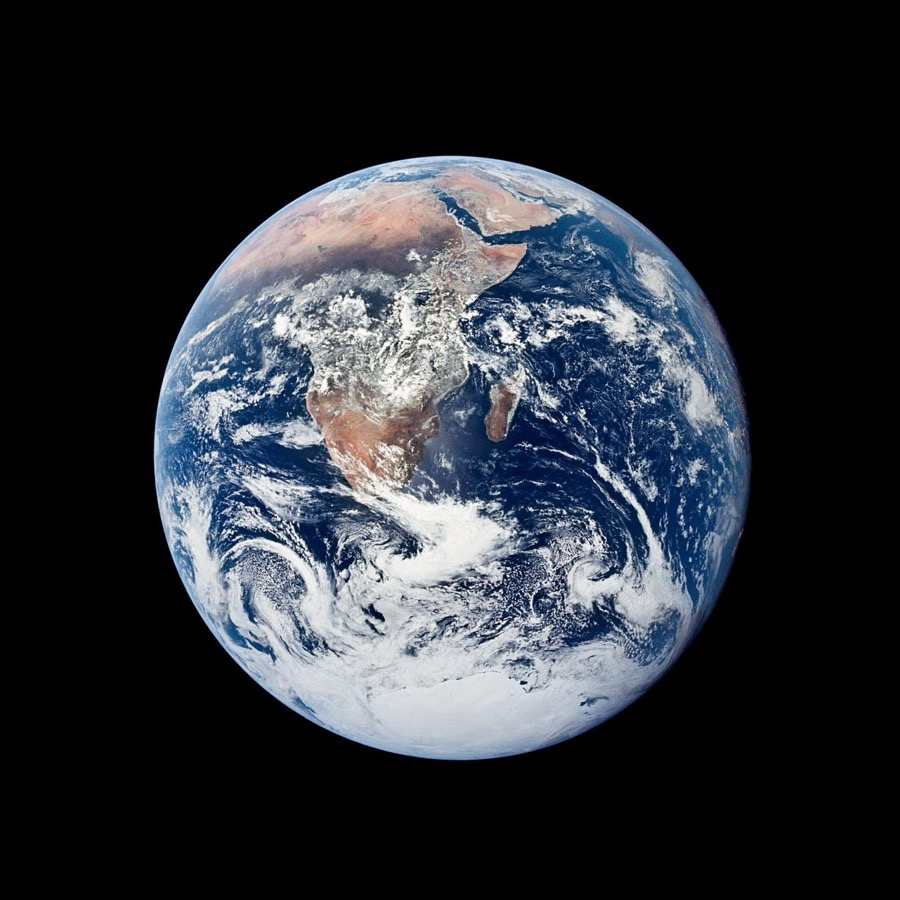
\includegraphics[width=0.55\linewidth]{images/blue-marble-nasa.jpg}
  \caption{Beispielabbildung mit Quellenangabe~\cite{nasa-blue-marble}}
  \label{abb:blue-marble}
\end{figure}

Vektorgrafiken haben gegenüber Screenshots den Vorteil, dass

\begin{itemize}
  \item sie jederzeit editiert werden können,
  \item sie beliebig skaliert werden können, ohne unscharf zu werden,
  \item alle Grafiken einheitlich vergrößert oder verkleinert werden können.
        Das verbessert das Layout ungemein.
\end{itemize}

Abbildungen stehen immer alleinstehend und zentriert. Die Breite wird
relativ zur Textbreite angegeben (\lstinline|width=0.75\linewidth|), damit
sie nie über den Satzspiegel hinausragt. Sollen mehrere Grafiken
nebeneinander stehen, verwendet dafür zwei \lstinline|minipage|-Umgebungen
innerhalb einer \lstinline|figure|.

Die Positionierung übernimmt \LaTeX. Die Angabe \lstinline|[htbp]| erlaubt
es, die Abbildung an die Stelle im Text, an den Seitenanfang, an das
Seitenende oder auf eine eigene Seite zu setzen. Eine Abbildung kann dadurch
auf der Folgeseite landen -- das ist beabsichtigt und kein Fehler.

\subsection{Beschriftungen}

Alle Grafiken und Tabellen sind zu beschriften und mit Quellenangaben zu
versehen. Im Text muss auf jede Abbildung und jede Tabelle Bezug genommen
werden.

Die Beschriftung erfolgt mit \lstinline|\caption| innerhalb der
\lstinline|figure|- bzw.\ \lstinline|table|-Umgebung. Nur so werden
Abbildungs- und Tabellenverzeichnis korrekt geführt. Bei Abbildungen steht
die Beschriftung unter der Grafik, bei Tabellen darüber; die Vorlage stellt
das automatisch richtig ein.

Abbildungen werden mit \enquote{Abb.} und Tabellen mit \enquote{Tab.}
bezeichnet. Auch das erledigt die Vorlage; die Nummerierung läuft
durchgehend und nicht kapitelweise. In englischsprachigen Diplomarbeiten
wird \enquote{Abb.} durch \enquote{Fig.} ersetzt -- dafür genügt die
Klassenoption \lstinline|englisch|.

Unmittelbar nach \lstinline|\caption| gehört ein \lstinline|\label|. Ohne
Label lässt sich die Abbildung später nicht referenzieren. Bewährt hat sich
ein Präfix je Objektart: \lstinline|abb:|, \lstinline|tab:| und
\lstinline|code:|.

\subsection{Querverweise}

Textpassagen, die sich auf andere Kapitel, Grafiken oder Tabellen beziehen,
müssen eine Referenz enthalten. Diese wird mit \lstinline|\ref| erzeugt und
enthält zumindest die Kategorie und die Nummer, also etwa
\lstinline|Abb.~\ref{abb:aufbau}|. Das geschützte Leerzeichen
\lstinline|~| verhindert, dass zwischen Bezeichnung und Nummer umgebrochen
wird.

Liegen referenzierender Text und referenziertes Objekt mehr als eine Seite
auseinander, ist zusätzlich die Seitenzahl mit \lstinline|\pageref|
anzugeben.

Anders als in Word müssen Querverweise und Verzeichnisse nicht manuell
aktualisiert werden. \LaTeX{} löst sie beim Übersetzen auf, benötigt dafür
aber mehrere Durchläufe. \lstinline|latexmk| (bzw.\ \lstinline|make pdf|)
wiederholt den Lauf so lange, bis sich nichts mehr ändert. Meldet das
Protokoll am Ende \enquote{There were undefined references}, fehlt ein
\lstinline|\label| oder es ist falsch geschrieben.

\subsection{Quellenangaben}

In wissenschaftlichen Arbeiten ist es verpflichtend, die Quelle jeder
Aussage anzugeben, die nicht von einem selbst stammt. Der Leser muss die
Möglichkeit haben, die Ausführungen des Autors nachzuprüfen.

Zu diesem Zweck müssen im Text der Diplomarbeit alle verwendeten Quellen
(Fachbücher, Fachzeitschriften, Herstellerunterlagen, Webseiten, \ldots)
angegeben werden. Dies geschieht am Ende des zitierten Textes durch Angabe
der Quelle. Informationen aus Lehrbüchern können als Allgemeinwissen
vorausgesetzt werden und müssen nicht zitiert werden.

Bei inhaltlichen Zitaten, dem Normalfall in technischen Arbeiten, wird der
Inhalt der Quelle nur sinngemäß wiedergegeben.

Bei wörtlichen Zitaten, die in technischen Arbeiten eher selten auftreten,
wird die wörtlich zitierte Textstelle zwischen Anführungszeichen gesetzt,
dahinter steht die Quellenangabe. Eigene Kommentare im Zitat oder
Verkürzungen werden in eckigen Klammern angegeben. Kurze Zitate stehen mit
\lstinline|\zitat| im Fließtext, längere in der Umgebung
\lstinline|zitatfreistehend|.

Beispiel für ein Zitat im Text der Diplomarbeit:
\zitat{[\ldots] kann in diesem Fall eine relationale Datenbank vorteilhaft
eingesetzt werden}~\cite{beispiel-buch}.

Beispiel für ein Zitat als eigener Absatz:

\begin{zitatfreistehend}
  \enquote{The basic guideline for citing online sources is to follow the
  standard citation for the citation, or add the DOI in place of page
  numbers if the source is not paginated.}~\cite{beispiel-artikel}
\end{zitatfreistehend}

Für Diplomarbeiten an der \ac{HTL} Donaustadt ist der IEEE-Zitierstil zu
verwenden. Jeder Quelle wird eine Nummer zugeordnet und in eckigen Klammern
angegeben. Diese Vorlage stellt den Stil bereits ein; zitiert wird mit
\lstinline|\cite{schluessel}|, wobei der Schlüssel aus
\lstinline|references.bib| stammt. Das Quellenverzeichnis wird daraus
automatisch erzeugt und enthält nur tatsächlich zitierte Einträge.

Zum Verwalten der Quellen empfiehlt sich Zotero mit dem Plug-in Better
BibTeX, das \lstinline|references.bib| bei jeder Änderung automatisch neu
exportiert.

Es gibt viele verschiedene Typen von Quellen. Tab.~\ref{tab:quellentypen}
zeigt die häufigsten, den passenden BibTeX-Eintragstyp und die
Informationen, die mindestens enthalten sein sollten.

\begin{table}[htbp]
  \centering
  \caption{Quellentypen}
  \label{tab:quellentypen}
  \begin{tabular}{@{}p{0.28\linewidth}p{0.16\linewidth}p{0.46\linewidth}@{}}
    \toprule
    \tabkopf{Quellentyp} & \tabkopf{Eintragstyp} &
      \tabkopf{wichtigste Informationen} \\
    \midrule
    Buch (auch E-Books, Broschüren) & \lstinline|@book| &
      Autor(en), Titel, Auflage, Verlag, Ort, ISBN \\
    Diplomarbeit, Dissertation & \lstinline|@thesis| &
      Autor(en), Titel, Institution, Ort, Datum \\
    Webseite (auch PDF) & \lstinline|@online| &
      Autor(en), Titel, URL, Abrufdatum (\lstinline|urldate|) \\
    Zeitschriftenartikel & \lstinline|@article| &
      Autor(en), Titel, Publikation, Band, Ausgabe, Seiten, Datum \\
    Verwendung von KI & \lstinline|@online| &
      siehe Anhang und die Vorgaben des Ministeriums~\cite{beispiel-online} \\
    \bottomrule
  \end{tabular}
\end{table}

\subsection{Befehle und Umgebungen}

In Word übernehmen Formatvorlagen das einheitliche Layout. In \LaTeX{}
erfüllen Befehle und Umgebungen dieselbe Aufgabe: Der Text beschreibt, was
etwas \emph{ist}, das Aussehen legt die Dokumentklasse \lstinline|htldon.cls|
zentral fest. Dadurch lässt sich die Formatierung nachträglich an einer
einzigen Stelle ändern.

Die in Tab.~\ref{tab:befehle} aufgeführten Befehle stellen sicher, dass alle
Diplomarbeiten den Richtlinien entsprechen. Sie dürfen nur in begründeten
Ausnahmefällen angepasst werden.

\begin{table}[htbp]
  \centering
  \caption{Befehle und Umgebungen der Vorlage}
  \label{tab:befehle}
  \begin{tabular}{@{}p{0.36\linewidth}p{0.58\linewidth}@{}}
    \toprule
    \tabkopf{Befehl} & \tabkopf{Beschreibung} \\
    \midrule
    \lstinline|\chapter| bis \lstinline|\subsubsection| &
      Kapitelüberschriften mit Dezimalklassifikation. Die ersten drei Ebenen
      erscheinen im Inhaltsverzeichnis, \lstinline|\subsubsection| nicht. \\
    \lstinline|\paragraph| &
      Zwischenüberschrift ohne Nummerierung, nicht im Inhaltsverzeichnis. \\
    \lstinline|\abschnittsautor| &
      Verfasser/in eines Abschnitts, erscheint rechts in der Kopfzeile.
      Format: erster Buchstabe des Vornamens, Punkt, Nachname
      (\enquote{M. Muster}). \\
    \lstinline|\zitat|, \lstinline|zitatfreistehend| &
      Kennzeichnung wörtlicher Zitate im Fließtext bzw.\ als eigener Absatz. \\
    \lstinline|\menue| &
      Menüstrukturen (\menue{Datei / Öffnen}) und Tastatureingaben
      (\menue{Strg + A}). \\
    \lstinline|lstlisting|, \lstinline|\lstinline| &
      Quellcode als eigener Block bzw.\ im Fließtext. \\
    \lstinline|\tabkopf| &
      Kopfzeile einer Tabelle. Der Tabelleninhalt selbst wird von der Klasse
      automatisch auf 10\,pt und linksbündig gestellt. \\
    \lstinline|\ac|, \lstinline|\acp| &
      Abkürzung, beim ersten Auftreten ausgeschrieben, im Plural mit
      \lstinline|\acp|. \\
    \lstinline|\cite|, \lstinline|\ref|, \lstinline|\pageref| &
      Quellenangabe, Querverweis, Seitenverweis. \\
    \bottomrule
  \end{tabular}
\end{table}

Überschriften der Kapitel müssen kurz, präzise und selbsterklärend sein.
Beispiele für unzureichende Überschriften: \enquote{5.3 Aufbau},
\enquote{5.3 Messergebnis}, \enquote{5.3 Beispiel}.

Bei Unterüberschriften gilt:

\begin{itemize}
  \item Es muss mindestens zwei Unterpunkte geben. Ein Abschnitt 3.2.1 darf
        daher nicht existieren, wenn kein 3.2.2 folgt.
  \item Unterpunkte sollten inhaltlich ausreichend gefüllt sein und
        mindestens eine halbe Seite umfassen.
  \item Unterpunkte, die lediglich aus einem einzelnen Satz bestehen, werden
        besser als Aufzählung dargestellt.
\end{itemize}

Für die Darstellung von Quellcode gilt:

\begin{itemize}
  \item Umfang:
        \begin{itemize}
          \item Der vollständige Sourcecode gehört ausschließlich auf das
                elektronische Speichermedium.
          \item Im Dokument selbst sollen nur wesentliche Ausschnitte
                aufgenommen werden.
        \end{itemize}
  \item Formatierung: Schriftart und Schriftgröße gibt die
        \lstinline|lstlisting|-Umgebung vor, der Zeilenabstand ist dort
        einzeilig. Die Sprache wird mit
        \lstinline|[language=Python]| angegeben, damit die
        Syntaxhervorhebung stimmt.
  \item Inhaltliche Anforderungen: Der Sourcecode muss ausreichend
        kommentiert sein.
  \item Verwendung im Fließtext: Wird Sourcecode im Text erwähnt, ist
        \lstinline|\lstinline| zu verwenden. Zusätzliche Anführungszeichen
        sind nicht erforderlich. Beispiel: Mit dem Befehl
        \lstinline|ShowModal| wird ein Frame geöffnet.
\end{itemize}

\section{Beschreibung der Kapitel}

\subsection{Titelseite}

Die Titelseite wird vollständig aus \lstinline|metadata.tex| erzeugt. Dort
sind einzutragen:

\begin{itemize}
  \item der Titel der Diplomarbeit mit \lstinline|\titel|. Er wird
        automatisch in die Kopfzeile übernommen.
  \item ein Projektlogo, Bild oder eine Zeichnung mit
        \lstinline|\projektlogo|.
  \item alle Verfasser/innen mit \lstinline|\teammitglied| und die
        Betreuung mit \lstinline|\betreuung|.
  \item Schuljahr, Abteilung und Klasse.
\end{itemize}

Falls alle Verfasser/innen oder Betreuer/innen dasselbe Geschlecht haben,
kann die geschlechtsspezifische Form verwendet werden; dafür ist das
optionale Argument von \lstinline|\betreuung| vorgesehen.

\subsection{Verfassererklärung}

In der Verfassererklärung bekennen sich die Verfasser/innen zu einem
wissenschaftlichen Arbeitsstil. Sollten im Nachhinein grobe Verstöße dagegen
aufgedeckt werden, kann die Arbeit für ungültig erklärt und der Abschluss
revidiert werden.

Die Erklärung erzeugt \lstinline|\eigenstaendigkeitserklaerung|. Je
Teammitglied entsteht automatisch eine Unterschriftszeile. Zu ergänzen sind
gegebenenfalls Kooperationen mit Firmen und Sperrvermerke.

\subsection{Problemstellung}

Die Seite \enquote{Problemstellung} wird durch den eingescannten Antrag (mit
allen Stempeln und Unterschriften) vollflächig ersetzt. Dazu wird in
\lstinline|frontmatter/problem-statement.tex| das Scan-PDF eingebunden.

\subsection{Kurzfassung bzw.\ Abstract}

Die Kurzfassung bzw.\ der Abstract soll kurz, prägnant und verständlich den
Inhalt der Arbeit wiedergeben: Zielsetzung, Ablauf, wichtigste Erkenntnisse,
wesentliche Merkmale des realisierten Produkts, Schlussfolgerungen und
Ausblick. Beide sind als eigenständiges Dokument zu konzipieren, das
unabhängig von der Diplomarbeit gelesen und verstanden werden kann, und
sollen in Deutsch und Englisch jeweils nicht mehr als eine Seite umfassen.

\subsection{Inhaltsverzeichnis}

Das Inhaltsverzeichnis wird automatisch aus den Überschriften erstellt. Es
zeigt die ersten drei Ebenen, der Text steht linksbündig, die Seitenzahlen
rechtsbündig, als Füllzeichen dienen Punkte. Eine manuelle Aktualisierung
ist nicht nötig.

\subsection{Die weiteren Kapitel}

Die Kapitel Projektplanung, Technische Grundlagen, Praktische Realisierung
sowie Evaluierung und Ergebnisse beschreiben die Diplomarbeit im Detail.

Für die Beurteilung ist es wichtig, den/die Verfasser/in zu kennen. Daher
ist dieser Hinweis auf jeder Seite rechtsbündig in der Kopfzeile zu
vermerken. Dafür wird \lstinline|\abschnittsautor| direkt nach der
Überschrift gesetzt; der Eintrag gilt ab dort bis zur nächsten Angabe.
Haben mehrere Personen gemeinsam an einem Abschnitt gearbeitet, sind alle zu
nennen, durch Komma getrennt:
\lstinline|\abschnittsautor{A. Erste, B. Zweite}|.

Die Projektplanung soll die systematische Durchführung der Diplomarbeit
innerhalb des Projektteams beschreiben. Dabei sollen geplante Ziele und
tatsächlich erreichte Ergebnisse miteinander verglichen und die Unterschiede
reflektiert werden. Beim klassischen Wasserfall-Projektmanagement können
etwa die Meilensteine als Referenz dienen, bei agiler Projektorganisation
die Sprint-Reviews.

Im Kapitel Technische Grundlagen finden sich alle für das unmittelbare
technische Verständnis der Diplomarbeit relevanten Inhalte. Hier wird
insbesondere auf korrekte Zitate und den sorgfältigen Einsatz von Quellen
geachtet.

Das Kapitel Praktische Realisierung enthält die praktischen Eigenleistungen
der Diplomarbeit. Dabei sollen die Vorgänge und Untersuchungen beschrieben
und nachvollziehbar dokumentiert werden.

Im Kapitel Evaluierung und Ergebnisse erfolgt die Darstellung und Bewertung
der abschließenden Arbeit. Hier soll ebenso, sofern vorhanden, das
Endprodukt bzw.\ der Prototyp präsentiert und beschrieben werden.

\subsection{Anhang}

Im Anhang können alle Informationen gesammelt werden, die zwar zur
Diplomarbeit gehören, jedoch im Inhaltsteil den Rahmen gesprengt hätten.
Dazu zählen wichtige Notizen (z.\,B. Gesprächsprotokolle), Normen,
Schnittstellendefinitionen oder Präsentationen. Weiters soll der Anhang den
Inhalt eines beigefügten elektronischen Speichermediums sowie einen
einseitigen Lebenslauf jedes Teammitglieds enthalten.

Verpflichtend ist außerdem die Dokumentation aller eingesetzten KI-basierten
Hilfsmittel. Dafür ist \lstinline|appendix/ai-tools.tex| vorgesehen.

% in diplomarbeit.tex entfernen und diese Datei mitlöschen.
% =====================================================================
\chapter{Richtlinie für das Verfassen von Diplomarbeiten}

Diese Richtlinie beschreibt die formalen und inhaltlichen Anforderungen an
eine wissenschaftliche Publikation und soll ein einheitliches
Erscheinungsbild der Diplomarbeiten sicherstellen. Dieses Kapitel beschreibt
weiters, wie die vorliegende Diplomarbeitsvorlage zu verwenden ist, und ist
im finalen Dokument zu entfernen.

Es sind bewusst nur die wesentlichen Punkte festgelegt. In Absprache mit dem
Betreuer/der Betreuerin soll stets Freiraum für die individuelle Gestaltung
sowie projektbedingte Erfordernisse bleiben.

\section{Allgemein}

Die Diplomarbeit soll kurz und prägnant -- aber vollständig -- gehalten sein
und einen Umfang von ca.\ 70 Seiten (ohne Anhang) bei einer Teamgröße von
2 Personen umfassen. Die inhaltliche Qualität bei in Umfang eingeschränkter
Darstellung ist ein wesentliches Ziel jeder wissenschaftlichen Publikation
und wird auch in die Beurteilung einbezogen. Grafische Darstellungen,
Übersichtstabellen und Diagramme sind wichtige Hilfsmittel, um diese Vorgabe
einhalten zu können.

Einige Tipps:

\begin{itemize}
  \item Das Verwenden der \enquote{ich}- und \enquote{wir}-Form sowie von
        \enquote{man}-Aussagen ist zu vermeiden.
  \item Abkürzungen müssen unmittelbar nach ihrem ersten Auftreten erläutert
        werden; falls erforderlich, ist ein Abkürzungsverzeichnis zu
        erstellen. Der Befehl \lstinline|\ac{API}| erledigt das automatisch:
        beim ersten Auftreten schreibt er die Abkürzung aus, danach nicht
        mehr.
  \item Über Themen, die nur indirekt mit der gestellten Aufgabe zu tun
        haben, soll nicht berichtet werden. Die ausführliche Darstellung von
        Grundlagenwissen ist nicht erforderlich; meistens reicht das Zitieren
        geeigneter Quellen.
  \item Arbeitet im Team über ein Git-Repository und legt pro Kapitel eine
        eigene Datei an. So lassen sich Änderungen nachvollziehen und
        Konflikte auf einzelne Absätze eingrenzen.
\end{itemize}

\subsection{Platzhalter in dieser Vorlage}

Alle Beispieltexte in dieser Vorlage sind zu ersetzen oder zu löschen. Das
betrifft insbesondere:

\begin{itemize}
  \item die Metadaten in \lstinline|metadata.tex| (Titel, Team, Betreuung,
        Schuljahr, Klasse),
  \item die Beispielkapitel in \lstinline|chapters/|,
  \item die Beispielquellen in \lstinline|references.bib|,
  \item das Abkürzungsverzeichnis in \lstinline|diplomarbeit.tex|,
  \item dieses gesamte Kapitel~6.
\end{itemize}

Um dieses Kapitel zu entfernen, genügt es, in \lstinline|diplomarbeit.tex|
die Zeile \lstinline|% =====================================================================
% Kapitel 6 der Abteilungsvorlage, auf LaTeX übertragen.
% Vor der Abgabe komplett löschen: die Zeile \input{chapters/06-guideline}
% in diplomarbeit.tex entfernen und diese Datei mitlöschen.
% =====================================================================
\chapter{Richtlinie für das Verfassen von Diplomarbeiten}

Diese Richtlinie beschreibt die formalen und inhaltlichen Anforderungen an
eine wissenschaftliche Publikation und soll ein einheitliches
Erscheinungsbild der Diplomarbeiten sicherstellen. Dieses Kapitel beschreibt
weiters, wie die vorliegende Diplomarbeitsvorlage zu verwenden ist, und ist
im finalen Dokument zu entfernen.

Es sind bewusst nur die wesentlichen Punkte festgelegt. In Absprache mit dem
Betreuer/der Betreuerin soll stets Freiraum für die individuelle Gestaltung
sowie projektbedingte Erfordernisse bleiben.

\section{Allgemein}

Die Diplomarbeit soll kurz und prägnant -- aber vollständig -- gehalten sein
und einen Umfang von ca.\ 70 Seiten (ohne Anhang) bei einer Teamgröße von
2 Personen umfassen. Die inhaltliche Qualität bei in Umfang eingeschränkter
Darstellung ist ein wesentliches Ziel jeder wissenschaftlichen Publikation
und wird auch in die Beurteilung einbezogen. Grafische Darstellungen,
Übersichtstabellen und Diagramme sind wichtige Hilfsmittel, um diese Vorgabe
einhalten zu können.

Einige Tipps:

\begin{itemize}
  \item Das Verwenden der \enquote{ich}- und \enquote{wir}-Form sowie von
        \enquote{man}-Aussagen ist zu vermeiden.
  \item Abkürzungen müssen unmittelbar nach ihrem ersten Auftreten erläutert
        werden; falls erforderlich, ist ein Abkürzungsverzeichnis zu
        erstellen. Der Befehl \lstinline|\ac{API}| erledigt das automatisch:
        beim ersten Auftreten schreibt er die Abkürzung aus, danach nicht
        mehr.
  \item Über Themen, die nur indirekt mit der gestellten Aufgabe zu tun
        haben, soll nicht berichtet werden. Die ausführliche Darstellung von
        Grundlagenwissen ist nicht erforderlich; meistens reicht das Zitieren
        geeigneter Quellen.
  \item Arbeitet im Team über ein Git-Repository und legt pro Kapitel eine
        eigene Datei an. So lassen sich Änderungen nachvollziehen und
        Konflikte auf einzelne Absätze eingrenzen.
\end{itemize}

\subsection{Platzhalter in dieser Vorlage}

Alle Beispieltexte in dieser Vorlage sind zu ersetzen oder zu löschen. Das
betrifft insbesondere:

\begin{itemize}
  \item die Metadaten in \lstinline|metadata.tex| (Titel, Team, Betreuung,
        Schuljahr, Klasse),
  \item die Beispielkapitel in \lstinline|chapters/|,
  \item die Beispielquellen in \lstinline|references.bib|,
  \item das Abkürzungsverzeichnis in \lstinline|diplomarbeit.tex|,
  \item dieses gesamte Kapitel~6.
\end{itemize}

Um dieses Kapitel zu entfernen, genügt es, in \lstinline|diplomarbeit.tex|
die Zeile \lstinline|\input{chapters/06-guideline}| zu löschen. Die Einträge
im Inhaltsverzeichnis und in den übrigen Verzeichnissen verschwinden beim
nächsten Übersetzen von selbst.

\subsection{Abgabe der Diplomarbeit}

Die Diplomarbeit ist in gedruckter bzw.\ gebundener Form und in digitaler
Form vorzulegen. Dem Abteilungsvorstand sind zwei geheftete Exemplare (ein
Belegexemplar und ein Beurteilungsexemplar für den/die Betreuer/in) zu
übergeben.

Nach erfolgter Beurteilung geht das Beurteilungsexemplar temporär zurück an
die Diplomarbeitsgruppe. Nun können letzte Korrekturen (ohne
Beurteilungsrelevanz) vorgenommen werden. Anschließend wird die Arbeit erneut
ausgedruckt und gesammelt zur Bindung außer Haus gegeben. Weitere Exemplare
für Kooperationspartner (Firmen, Institutionen) oder Projektteilnehmer können
in diesem Zusammenhang erstellt werden.

\subsection{Grafiken}

Abbildungen müssen in gut lesbarer Bildqualität eingefügt werden. Grafiken
sollten am besten in einem vektorbasierten Zeichenprogramm (z.\,B. Inkscape,
draw.io) erstellt und als PDF exportiert werden; PDF und PNG lassen sich
direkt einbinden, SVG nicht. Alle Bilddateien gehören in den Ordner
\lstinline|images/|.

\begin{lstlisting}[language={[LaTeX]TeX}, caption={Eine Abbildung einbinden},
                   label=code:abbildung]
\begin{figure}[htbp]
  \centering
  
\includegraphics[width=0.75\linewidth]{images/example-figure.pdf}
  \caption{Aufbau des Systems}
  \label{abb:aufbau}
\end{figure}
\end{lstlisting}

Abb.~\ref{abb:blue-marble} zeigt, wie das Ergebnis aussieht. Stammt die
Grafik nicht von euch selbst, gehört die Quelle in die Beschriftung.

\begin{figure}[htbp]
  \centering
  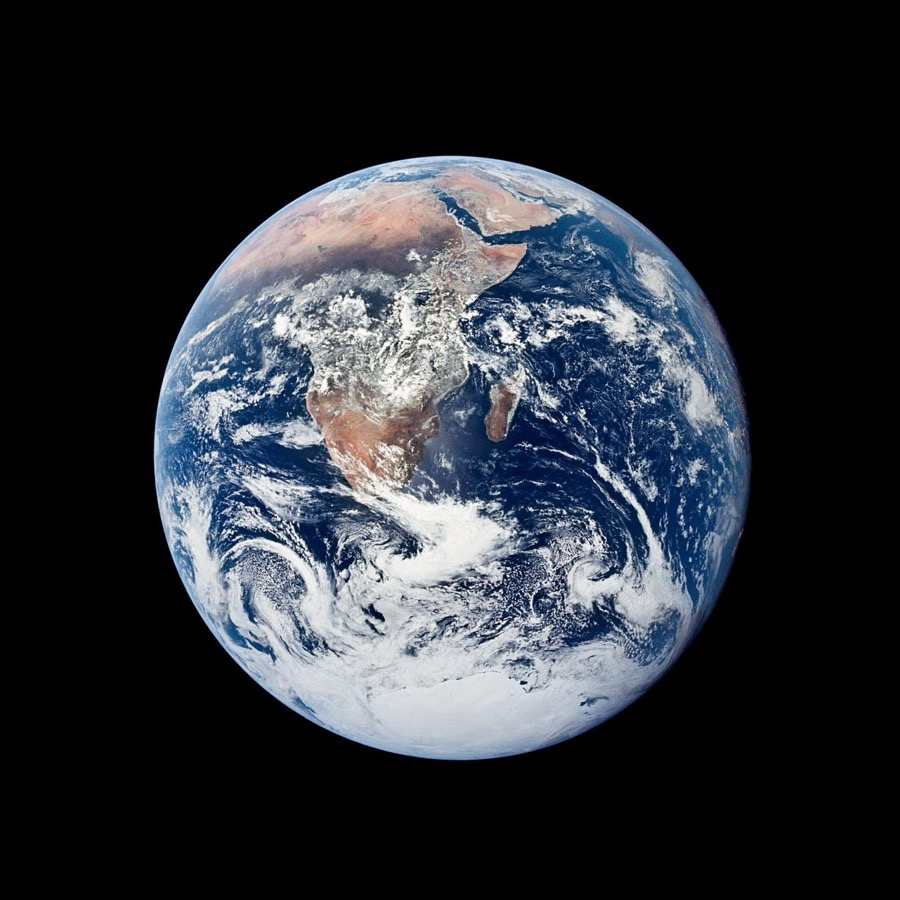
\includegraphics[width=0.55\linewidth]{images/blue-marble-nasa.jpg}
  \caption{Beispielabbildung mit Quellenangabe~\cite{nasa-blue-marble}}
  \label{abb:blue-marble}
\end{figure}

Vektorgrafiken haben gegenüber Screenshots den Vorteil, dass

\begin{itemize}
  \item sie jederzeit editiert werden können,
  \item sie beliebig skaliert werden können, ohne unscharf zu werden,
  \item alle Grafiken einheitlich vergrößert oder verkleinert werden können.
        Das verbessert das Layout ungemein.
\end{itemize}

Abbildungen stehen immer alleinstehend und zentriert. Die Breite wird
relativ zur Textbreite angegeben (\lstinline|width=0.75\linewidth|), damit
sie nie über den Satzspiegel hinausragt. Sollen mehrere Grafiken
nebeneinander stehen, verwendet dafür zwei \lstinline|minipage|-Umgebungen
innerhalb einer \lstinline|figure|.

Die Positionierung übernimmt \LaTeX. Die Angabe \lstinline|[htbp]| erlaubt
es, die Abbildung an die Stelle im Text, an den Seitenanfang, an das
Seitenende oder auf eine eigene Seite zu setzen. Eine Abbildung kann dadurch
auf der Folgeseite landen -- das ist beabsichtigt und kein Fehler.

\subsection{Beschriftungen}

Alle Grafiken und Tabellen sind zu beschriften und mit Quellenangaben zu
versehen. Im Text muss auf jede Abbildung und jede Tabelle Bezug genommen
werden.

Die Beschriftung erfolgt mit \lstinline|\caption| innerhalb der
\lstinline|figure|- bzw.\ \lstinline|table|-Umgebung. Nur so werden
Abbildungs- und Tabellenverzeichnis korrekt geführt. Bei Abbildungen steht
die Beschriftung unter der Grafik, bei Tabellen darüber; die Vorlage stellt
das automatisch richtig ein.

Abbildungen werden mit \enquote{Abb.} und Tabellen mit \enquote{Tab.}
bezeichnet. Auch das erledigt die Vorlage; die Nummerierung läuft
durchgehend und nicht kapitelweise. In englischsprachigen Diplomarbeiten
wird \enquote{Abb.} durch \enquote{Fig.} ersetzt -- dafür genügt die
Klassenoption \lstinline|englisch|.

Unmittelbar nach \lstinline|\caption| gehört ein \lstinline|\label|. Ohne
Label lässt sich die Abbildung später nicht referenzieren. Bewährt hat sich
ein Präfix je Objektart: \lstinline|abb:|, \lstinline|tab:| und
\lstinline|code:|.

\subsection{Querverweise}

Textpassagen, die sich auf andere Kapitel, Grafiken oder Tabellen beziehen,
müssen eine Referenz enthalten. Diese wird mit \lstinline|\ref| erzeugt und
enthält zumindest die Kategorie und die Nummer, also etwa
\lstinline|Abb.~\ref{abb:aufbau}|. Das geschützte Leerzeichen
\lstinline|~| verhindert, dass zwischen Bezeichnung und Nummer umgebrochen
wird.

Liegen referenzierender Text und referenziertes Objekt mehr als eine Seite
auseinander, ist zusätzlich die Seitenzahl mit \lstinline|\pageref|
anzugeben.

Anders als in Word müssen Querverweise und Verzeichnisse nicht manuell
aktualisiert werden. \LaTeX{} löst sie beim Übersetzen auf, benötigt dafür
aber mehrere Durchläufe. \lstinline|latexmk| (bzw.\ \lstinline|make pdf|)
wiederholt den Lauf so lange, bis sich nichts mehr ändert. Meldet das
Protokoll am Ende \enquote{There were undefined references}, fehlt ein
\lstinline|\label| oder es ist falsch geschrieben.

\subsection{Quellenangaben}

In wissenschaftlichen Arbeiten ist es verpflichtend, die Quelle jeder
Aussage anzugeben, die nicht von einem selbst stammt. Der Leser muss die
Möglichkeit haben, die Ausführungen des Autors nachzuprüfen.

Zu diesem Zweck müssen im Text der Diplomarbeit alle verwendeten Quellen
(Fachbücher, Fachzeitschriften, Herstellerunterlagen, Webseiten, \ldots)
angegeben werden. Dies geschieht am Ende des zitierten Textes durch Angabe
der Quelle. Informationen aus Lehrbüchern können als Allgemeinwissen
vorausgesetzt werden und müssen nicht zitiert werden.

Bei inhaltlichen Zitaten, dem Normalfall in technischen Arbeiten, wird der
Inhalt der Quelle nur sinngemäß wiedergegeben.

Bei wörtlichen Zitaten, die in technischen Arbeiten eher selten auftreten,
wird die wörtlich zitierte Textstelle zwischen Anführungszeichen gesetzt,
dahinter steht die Quellenangabe. Eigene Kommentare im Zitat oder
Verkürzungen werden in eckigen Klammern angegeben. Kurze Zitate stehen mit
\lstinline|\zitat| im Fließtext, längere in der Umgebung
\lstinline|zitatfreistehend|.

Beispiel für ein Zitat im Text der Diplomarbeit:
\zitat{[\ldots] kann in diesem Fall eine relationale Datenbank vorteilhaft
eingesetzt werden}~\cite{beispiel-buch}.

Beispiel für ein Zitat als eigener Absatz:

\begin{zitatfreistehend}
  \enquote{The basic guideline for citing online sources is to follow the
  standard citation for the citation, or add the DOI in place of page
  numbers if the source is not paginated.}~\cite{beispiel-artikel}
\end{zitatfreistehend}

Für Diplomarbeiten an der \ac{HTL} Donaustadt ist der IEEE-Zitierstil zu
verwenden. Jeder Quelle wird eine Nummer zugeordnet und in eckigen Klammern
angegeben. Diese Vorlage stellt den Stil bereits ein; zitiert wird mit
\lstinline|\cite{schluessel}|, wobei der Schlüssel aus
\lstinline|references.bib| stammt. Das Quellenverzeichnis wird daraus
automatisch erzeugt und enthält nur tatsächlich zitierte Einträge.

Zum Verwalten der Quellen empfiehlt sich Zotero mit dem Plug-in Better
BibTeX, das \lstinline|references.bib| bei jeder Änderung automatisch neu
exportiert.

Es gibt viele verschiedene Typen von Quellen. Tab.~\ref{tab:quellentypen}
zeigt die häufigsten, den passenden BibTeX-Eintragstyp und die
Informationen, die mindestens enthalten sein sollten.

\begin{table}[htbp]
  \centering
  \caption{Quellentypen}
  \label{tab:quellentypen}
  \begin{tabular}{@{}p{0.28\linewidth}p{0.16\linewidth}p{0.46\linewidth}@{}}
    \toprule
    \tabkopf{Quellentyp} & \tabkopf{Eintragstyp} &
      \tabkopf{wichtigste Informationen} \\
    \midrule
    Buch (auch E-Books, Broschüren) & \lstinline|@book| &
      Autor(en), Titel, Auflage, Verlag, Ort, ISBN \\
    Diplomarbeit, Dissertation & \lstinline|@thesis| &
      Autor(en), Titel, Institution, Ort, Datum \\
    Webseite (auch PDF) & \lstinline|@online| &
      Autor(en), Titel, URL, Abrufdatum (\lstinline|urldate|) \\
    Zeitschriftenartikel & \lstinline|@article| &
      Autor(en), Titel, Publikation, Band, Ausgabe, Seiten, Datum \\
    Verwendung von KI & \lstinline|@online| &
      siehe Anhang und die Vorgaben des Ministeriums~\cite{beispiel-online} \\
    \bottomrule
  \end{tabular}
\end{table}

\subsection{Befehle und Umgebungen}

In Word übernehmen Formatvorlagen das einheitliche Layout. In \LaTeX{}
erfüllen Befehle und Umgebungen dieselbe Aufgabe: Der Text beschreibt, was
etwas \emph{ist}, das Aussehen legt die Dokumentklasse \lstinline|htldon.cls|
zentral fest. Dadurch lässt sich die Formatierung nachträglich an einer
einzigen Stelle ändern.

Die in Tab.~\ref{tab:befehle} aufgeführten Befehle stellen sicher, dass alle
Diplomarbeiten den Richtlinien entsprechen. Sie dürfen nur in begründeten
Ausnahmefällen angepasst werden.

\begin{table}[htbp]
  \centering
  \caption{Befehle und Umgebungen der Vorlage}
  \label{tab:befehle}
  \begin{tabular}{@{}p{0.36\linewidth}p{0.58\linewidth}@{}}
    \toprule
    \tabkopf{Befehl} & \tabkopf{Beschreibung} \\
    \midrule
    \lstinline|\chapter| bis \lstinline|\subsubsection| &
      Kapitelüberschriften mit Dezimalklassifikation. Die ersten drei Ebenen
      erscheinen im Inhaltsverzeichnis, \lstinline|\subsubsection| nicht. \\
    \lstinline|\paragraph| &
      Zwischenüberschrift ohne Nummerierung, nicht im Inhaltsverzeichnis. \\
    \lstinline|\abschnittsautor| &
      Verfasser/in eines Abschnitts, erscheint rechts in der Kopfzeile.
      Format: erster Buchstabe des Vornamens, Punkt, Nachname
      (\enquote{M. Muster}). \\
    \lstinline|\zitat|, \lstinline|zitatfreistehend| &
      Kennzeichnung wörtlicher Zitate im Fließtext bzw.\ als eigener Absatz. \\
    \lstinline|\menue| &
      Menüstrukturen (\menue{Datei / Öffnen}) und Tastatureingaben
      (\menue{Strg + A}). \\
    \lstinline|lstlisting|, \lstinline|\lstinline| &
      Quellcode als eigener Block bzw.\ im Fließtext. \\
    \lstinline|\tabkopf| &
      Kopfzeile einer Tabelle. Der Tabelleninhalt selbst wird von der Klasse
      automatisch auf 10\,pt und linksbündig gestellt. \\
    \lstinline|\ac|, \lstinline|\acp| &
      Abkürzung, beim ersten Auftreten ausgeschrieben, im Plural mit
      \lstinline|\acp|. \\
    \lstinline|\cite|, \lstinline|\ref|, \lstinline|\pageref| &
      Quellenangabe, Querverweis, Seitenverweis. \\
    \bottomrule
  \end{tabular}
\end{table}

Überschriften der Kapitel müssen kurz, präzise und selbsterklärend sein.
Beispiele für unzureichende Überschriften: \enquote{5.3 Aufbau},
\enquote{5.3 Messergebnis}, \enquote{5.3 Beispiel}.

Bei Unterüberschriften gilt:

\begin{itemize}
  \item Es muss mindestens zwei Unterpunkte geben. Ein Abschnitt 3.2.1 darf
        daher nicht existieren, wenn kein 3.2.2 folgt.
  \item Unterpunkte sollten inhaltlich ausreichend gefüllt sein und
        mindestens eine halbe Seite umfassen.
  \item Unterpunkte, die lediglich aus einem einzelnen Satz bestehen, werden
        besser als Aufzählung dargestellt.
\end{itemize}

Für die Darstellung von Quellcode gilt:

\begin{itemize}
  \item Umfang:
        \begin{itemize}
          \item Der vollständige Sourcecode gehört ausschließlich auf das
                elektronische Speichermedium.
          \item Im Dokument selbst sollen nur wesentliche Ausschnitte
                aufgenommen werden.
        \end{itemize}
  \item Formatierung: Schriftart und Schriftgröße gibt die
        \lstinline|lstlisting|-Umgebung vor, der Zeilenabstand ist dort
        einzeilig. Die Sprache wird mit
        \lstinline|[language=Python]| angegeben, damit die
        Syntaxhervorhebung stimmt.
  \item Inhaltliche Anforderungen: Der Sourcecode muss ausreichend
        kommentiert sein.
  \item Verwendung im Fließtext: Wird Sourcecode im Text erwähnt, ist
        \lstinline|\lstinline| zu verwenden. Zusätzliche Anführungszeichen
        sind nicht erforderlich. Beispiel: Mit dem Befehl
        \lstinline|ShowModal| wird ein Frame geöffnet.
\end{itemize}

\section{Beschreibung der Kapitel}

\subsection{Titelseite}

Die Titelseite wird vollständig aus \lstinline|metadata.tex| erzeugt. Dort
sind einzutragen:

\begin{itemize}
  \item der Titel der Diplomarbeit mit \lstinline|\titel|. Er wird
        automatisch in die Kopfzeile übernommen.
  \item ein Projektlogo, Bild oder eine Zeichnung mit
        \lstinline|\projektlogo|.
  \item alle Verfasser/innen mit \lstinline|\teammitglied| und die
        Betreuung mit \lstinline|\betreuung|.
  \item Schuljahr, Abteilung und Klasse.
\end{itemize}

Falls alle Verfasser/innen oder Betreuer/innen dasselbe Geschlecht haben,
kann die geschlechtsspezifische Form verwendet werden; dafür ist das
optionale Argument von \lstinline|\betreuung| vorgesehen.

\subsection{Verfassererklärung}

In der Verfassererklärung bekennen sich die Verfasser/innen zu einem
wissenschaftlichen Arbeitsstil. Sollten im Nachhinein grobe Verstöße dagegen
aufgedeckt werden, kann die Arbeit für ungültig erklärt und der Abschluss
revidiert werden.

Die Erklärung erzeugt \lstinline|\eigenstaendigkeitserklaerung|. Je
Teammitglied entsteht automatisch eine Unterschriftszeile. Zu ergänzen sind
gegebenenfalls Kooperationen mit Firmen und Sperrvermerke.

\subsection{Problemstellung}

Die Seite \enquote{Problemstellung} wird durch den eingescannten Antrag (mit
allen Stempeln und Unterschriften) vollflächig ersetzt. Dazu wird in
\lstinline|frontmatter/problem-statement.tex| das Scan-PDF eingebunden.

\subsection{Kurzfassung bzw.\ Abstract}

Die Kurzfassung bzw.\ der Abstract soll kurz, prägnant und verständlich den
Inhalt der Arbeit wiedergeben: Zielsetzung, Ablauf, wichtigste Erkenntnisse,
wesentliche Merkmale des realisierten Produkts, Schlussfolgerungen und
Ausblick. Beide sind als eigenständiges Dokument zu konzipieren, das
unabhängig von der Diplomarbeit gelesen und verstanden werden kann, und
sollen in Deutsch und Englisch jeweils nicht mehr als eine Seite umfassen.

\subsection{Inhaltsverzeichnis}

Das Inhaltsverzeichnis wird automatisch aus den Überschriften erstellt. Es
zeigt die ersten drei Ebenen, der Text steht linksbündig, die Seitenzahlen
rechtsbündig, als Füllzeichen dienen Punkte. Eine manuelle Aktualisierung
ist nicht nötig.

\subsection{Die weiteren Kapitel}

Die Kapitel Projektplanung, Technische Grundlagen, Praktische Realisierung
sowie Evaluierung und Ergebnisse beschreiben die Diplomarbeit im Detail.

Für die Beurteilung ist es wichtig, den/die Verfasser/in zu kennen. Daher
ist dieser Hinweis auf jeder Seite rechtsbündig in der Kopfzeile zu
vermerken. Dafür wird \lstinline|\abschnittsautor| direkt nach der
Überschrift gesetzt; der Eintrag gilt ab dort bis zur nächsten Angabe.
Haben mehrere Personen gemeinsam an einem Abschnitt gearbeitet, sind alle zu
nennen, durch Komma getrennt:
\lstinline|\abschnittsautor{A. Erste, B. Zweite}|.

Die Projektplanung soll die systematische Durchführung der Diplomarbeit
innerhalb des Projektteams beschreiben. Dabei sollen geplante Ziele und
tatsächlich erreichte Ergebnisse miteinander verglichen und die Unterschiede
reflektiert werden. Beim klassischen Wasserfall-Projektmanagement können
etwa die Meilensteine als Referenz dienen, bei agiler Projektorganisation
die Sprint-Reviews.

Im Kapitel Technische Grundlagen finden sich alle für das unmittelbare
technische Verständnis der Diplomarbeit relevanten Inhalte. Hier wird
insbesondere auf korrekte Zitate und den sorgfältigen Einsatz von Quellen
geachtet.

Das Kapitel Praktische Realisierung enthält die praktischen Eigenleistungen
der Diplomarbeit. Dabei sollen die Vorgänge und Untersuchungen beschrieben
und nachvollziehbar dokumentiert werden.

Im Kapitel Evaluierung und Ergebnisse erfolgt die Darstellung und Bewertung
der abschließenden Arbeit. Hier soll ebenso, sofern vorhanden, das
Endprodukt bzw.\ der Prototyp präsentiert und beschrieben werden.

\subsection{Anhang}

Im Anhang können alle Informationen gesammelt werden, die zwar zur
Diplomarbeit gehören, jedoch im Inhaltsteil den Rahmen gesprengt hätten.
Dazu zählen wichtige Notizen (z.\,B. Gesprächsprotokolle), Normen,
Schnittstellendefinitionen oder Präsentationen. Weiters soll der Anhang den
Inhalt eines beigefügten elektronischen Speichermediums sowie einen
einseitigen Lebenslauf jedes Teammitglieds enthalten.

Verpflichtend ist außerdem die Dokumentation aller eingesetzten KI-basierten
Hilfsmittel. Dafür ist \lstinline|appendix/ai-tools.tex| vorgesehen.
| zu löschen. Die Einträge
im Inhaltsverzeichnis und in den übrigen Verzeichnissen verschwinden beim
nächsten Übersetzen von selbst.

\subsection{Abgabe der Diplomarbeit}

Die Diplomarbeit ist in gedruckter bzw.\ gebundener Form und in digitaler
Form vorzulegen. Dem Abteilungsvorstand sind zwei geheftete Exemplare (ein
Belegexemplar und ein Beurteilungsexemplar für den/die Betreuer/in) zu
übergeben.

Nach erfolgter Beurteilung geht das Beurteilungsexemplar temporär zurück an
die Diplomarbeitsgruppe. Nun können letzte Korrekturen (ohne
Beurteilungsrelevanz) vorgenommen werden. Anschließend wird die Arbeit erneut
ausgedruckt und gesammelt zur Bindung außer Haus gegeben. Weitere Exemplare
für Kooperationspartner (Firmen, Institutionen) oder Projektteilnehmer können
in diesem Zusammenhang erstellt werden.

\subsection{Grafiken}

Abbildungen müssen in gut lesbarer Bildqualität eingefügt werden. Grafiken
sollten am besten in einem vektorbasierten Zeichenprogramm (z.\,B. Inkscape,
draw.io) erstellt und als PDF exportiert werden; PDF und PNG lassen sich
direkt einbinden, SVG nicht. Alle Bilddateien gehören in den Ordner
\lstinline|images/|.

\begin{lstlisting}[language={[LaTeX]TeX}, caption={Eine Abbildung einbinden},
                   label=code:abbildung]
\begin{figure}[htbp]
  \centering
  
\includegraphics[width=0.75\linewidth]{images/example-figure.pdf}
  \caption{Aufbau des Systems}
  \label{abb:aufbau}
\end{figure}
\end{lstlisting}

Abb.~\ref{abb:blue-marble} zeigt, wie das Ergebnis aussieht. Stammt die
Grafik nicht von euch selbst, gehört die Quelle in die Beschriftung.

\begin{figure}[htbp]
  \centering
  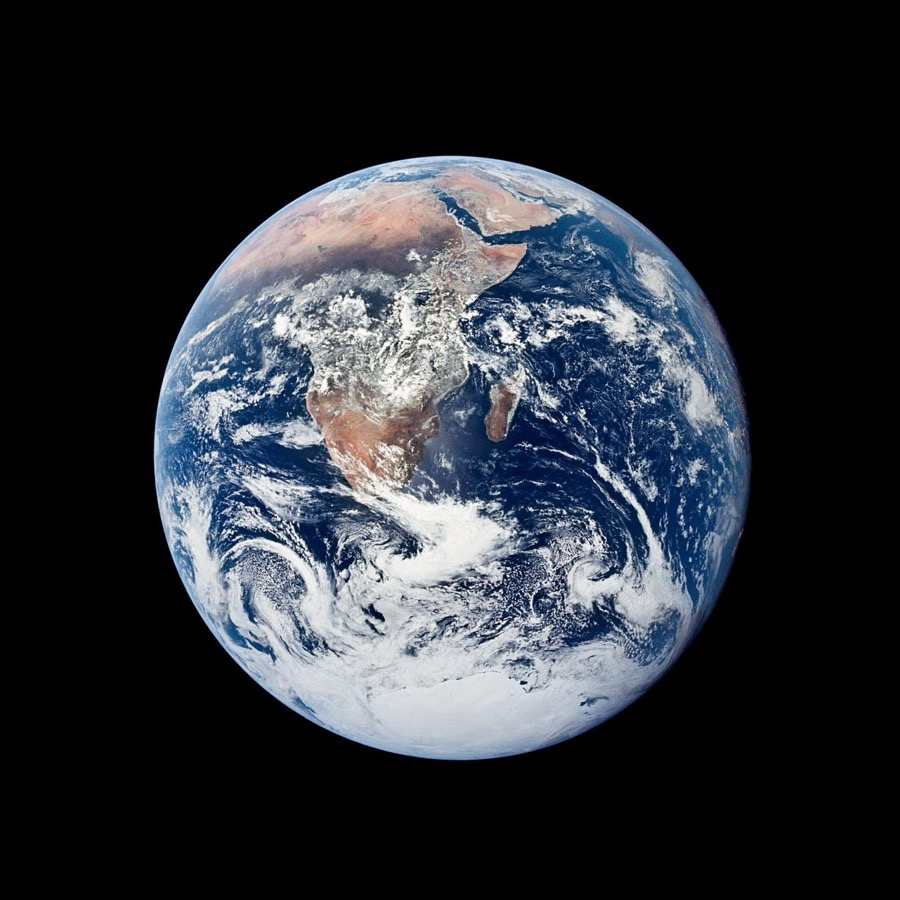
\includegraphics[width=0.55\linewidth]{images/blue-marble-nasa.jpg}
  \caption{Beispielabbildung mit Quellenangabe~\cite{nasa-blue-marble}}
  \label{abb:blue-marble}
\end{figure}

Vektorgrafiken haben gegenüber Screenshots den Vorteil, dass

\begin{itemize}
  \item sie jederzeit editiert werden können,
  \item sie beliebig skaliert werden können, ohne unscharf zu werden,
  \item alle Grafiken einheitlich vergrößert oder verkleinert werden können.
        Das verbessert das Layout ungemein.
\end{itemize}

Abbildungen stehen immer alleinstehend und zentriert. Die Breite wird
relativ zur Textbreite angegeben (\lstinline|width=0.75\linewidth|), damit
sie nie über den Satzspiegel hinausragt. Sollen mehrere Grafiken
nebeneinander stehen, verwendet dafür zwei \lstinline|minipage|-Umgebungen
innerhalb einer \lstinline|figure|.

Die Positionierung übernimmt \LaTeX. Die Angabe \lstinline|[htbp]| erlaubt
es, die Abbildung an die Stelle im Text, an den Seitenanfang, an das
Seitenende oder auf eine eigene Seite zu setzen. Eine Abbildung kann dadurch
auf der Folgeseite landen -- das ist beabsichtigt und kein Fehler.

\subsection{Beschriftungen}

Alle Grafiken und Tabellen sind zu beschriften und mit Quellenangaben zu
versehen. Im Text muss auf jede Abbildung und jede Tabelle Bezug genommen
werden.

Die Beschriftung erfolgt mit \lstinline|\caption| innerhalb der
\lstinline|figure|- bzw.\ \lstinline|table|-Umgebung. Nur so werden
Abbildungs- und Tabellenverzeichnis korrekt geführt. Bei Abbildungen steht
die Beschriftung unter der Grafik, bei Tabellen darüber; die Vorlage stellt
das automatisch richtig ein.

Abbildungen werden mit \enquote{Abb.} und Tabellen mit \enquote{Tab.}
bezeichnet. Auch das erledigt die Vorlage; die Nummerierung läuft
durchgehend und nicht kapitelweise. In englischsprachigen Diplomarbeiten
wird \enquote{Abb.} durch \enquote{Fig.} ersetzt -- dafür genügt die
Klassenoption \lstinline|englisch|.

Unmittelbar nach \lstinline|\caption| gehört ein \lstinline|\label|. Ohne
Label lässt sich die Abbildung später nicht referenzieren. Bewährt hat sich
ein Präfix je Objektart: \lstinline|abb:|, \lstinline|tab:| und
\lstinline|code:|.

\subsection{Querverweise}

Textpassagen, die sich auf andere Kapitel, Grafiken oder Tabellen beziehen,
müssen eine Referenz enthalten. Diese wird mit \lstinline|\ref| erzeugt und
enthält zumindest die Kategorie und die Nummer, also etwa
\lstinline|Abb.~\ref{abb:aufbau}|. Das geschützte Leerzeichen
\lstinline|~| verhindert, dass zwischen Bezeichnung und Nummer umgebrochen
wird.

Liegen referenzierender Text und referenziertes Objekt mehr als eine Seite
auseinander, ist zusätzlich die Seitenzahl mit \lstinline|\pageref|
anzugeben.

Anders als in Word müssen Querverweise und Verzeichnisse nicht manuell
aktualisiert werden. \LaTeX{} löst sie beim Übersetzen auf, benötigt dafür
aber mehrere Durchläufe. \lstinline|latexmk| (bzw.\ \lstinline|make pdf|)
wiederholt den Lauf so lange, bis sich nichts mehr ändert. Meldet das
Protokoll am Ende \enquote{There were undefined references}, fehlt ein
\lstinline|\label| oder es ist falsch geschrieben.

\subsection{Quellenangaben}

In wissenschaftlichen Arbeiten ist es verpflichtend, die Quelle jeder
Aussage anzugeben, die nicht von einem selbst stammt. Der Leser muss die
Möglichkeit haben, die Ausführungen des Autors nachzuprüfen.

Zu diesem Zweck müssen im Text der Diplomarbeit alle verwendeten Quellen
(Fachbücher, Fachzeitschriften, Herstellerunterlagen, Webseiten, \ldots)
angegeben werden. Dies geschieht am Ende des zitierten Textes durch Angabe
der Quelle. Informationen aus Lehrbüchern können als Allgemeinwissen
vorausgesetzt werden und müssen nicht zitiert werden.

Bei inhaltlichen Zitaten, dem Normalfall in technischen Arbeiten, wird der
Inhalt der Quelle nur sinngemäß wiedergegeben.

Bei wörtlichen Zitaten, die in technischen Arbeiten eher selten auftreten,
wird die wörtlich zitierte Textstelle zwischen Anführungszeichen gesetzt,
dahinter steht die Quellenangabe. Eigene Kommentare im Zitat oder
Verkürzungen werden in eckigen Klammern angegeben. Kurze Zitate stehen mit
\lstinline|\zitat| im Fließtext, längere in der Umgebung
\lstinline|zitatfreistehend|.

Beispiel für ein Zitat im Text der Diplomarbeit:
\zitat{[\ldots] kann in diesem Fall eine relationale Datenbank vorteilhaft
eingesetzt werden}~\cite{beispiel-buch}.

Beispiel für ein Zitat als eigener Absatz:

\begin{zitatfreistehend}
  \enquote{The basic guideline for citing online sources is to follow the
  standard citation for the citation, or add the DOI in place of page
  numbers if the source is not paginated.}~\cite{beispiel-artikel}
\end{zitatfreistehend}

Für Diplomarbeiten an der \ac{HTL} Donaustadt ist der IEEE-Zitierstil zu
verwenden. Jeder Quelle wird eine Nummer zugeordnet und in eckigen Klammern
angegeben. Diese Vorlage stellt den Stil bereits ein; zitiert wird mit
\lstinline|\cite{schluessel}|, wobei der Schlüssel aus
\lstinline|references.bib| stammt. Das Quellenverzeichnis wird daraus
automatisch erzeugt und enthält nur tatsächlich zitierte Einträge.

Zum Verwalten der Quellen empfiehlt sich Zotero mit dem Plug-in Better
BibTeX, das \lstinline|references.bib| bei jeder Änderung automatisch neu
exportiert.

Es gibt viele verschiedene Typen von Quellen. Tab.~\ref{tab:quellentypen}
zeigt die häufigsten, den passenden BibTeX-Eintragstyp und die
Informationen, die mindestens enthalten sein sollten.

\begin{table}[htbp]
  \centering
  \caption{Quellentypen}
  \label{tab:quellentypen}
  \begin{tabular}{@{}p{0.28\linewidth}p{0.16\linewidth}p{0.46\linewidth}@{}}
    \toprule
    \tabkopf{Quellentyp} & \tabkopf{Eintragstyp} &
      \tabkopf{wichtigste Informationen} \\
    \midrule
    Buch (auch E-Books, Broschüren) & \lstinline|@book| &
      Autor(en), Titel, Auflage, Verlag, Ort, ISBN \\
    Diplomarbeit, Dissertation & \lstinline|@thesis| &
      Autor(en), Titel, Institution, Ort, Datum \\
    Webseite (auch PDF) & \lstinline|@online| &
      Autor(en), Titel, URL, Abrufdatum (\lstinline|urldate|) \\
    Zeitschriftenartikel & \lstinline|@article| &
      Autor(en), Titel, Publikation, Band, Ausgabe, Seiten, Datum \\
    Verwendung von KI & \lstinline|@online| &
      siehe Anhang und die Vorgaben des Ministeriums~\cite{beispiel-online} \\
    \bottomrule
  \end{tabular}
\end{table}

\subsection{Befehle und Umgebungen}

In Word übernehmen Formatvorlagen das einheitliche Layout. In \LaTeX{}
erfüllen Befehle und Umgebungen dieselbe Aufgabe: Der Text beschreibt, was
etwas \emph{ist}, das Aussehen legt die Dokumentklasse \lstinline|htldon.cls|
zentral fest. Dadurch lässt sich die Formatierung nachträglich an einer
einzigen Stelle ändern.

Die in Tab.~\ref{tab:befehle} aufgeführten Befehle stellen sicher, dass alle
Diplomarbeiten den Richtlinien entsprechen. Sie dürfen nur in begründeten
Ausnahmefällen angepasst werden.

\begin{table}[htbp]
  \centering
  \caption{Befehle und Umgebungen der Vorlage}
  \label{tab:befehle}
  \begin{tabular}{@{}p{0.36\linewidth}p{0.58\linewidth}@{}}
    \toprule
    \tabkopf{Befehl} & \tabkopf{Beschreibung} \\
    \midrule
    \lstinline|\chapter| bis \lstinline|\subsubsection| &
      Kapitelüberschriften mit Dezimalklassifikation. Die ersten drei Ebenen
      erscheinen im Inhaltsverzeichnis, \lstinline|\subsubsection| nicht. \\
    \lstinline|\paragraph| &
      Zwischenüberschrift ohne Nummerierung, nicht im Inhaltsverzeichnis. \\
    \lstinline|\abschnittsautor| &
      Verfasser/in eines Abschnitts, erscheint rechts in der Kopfzeile.
      Format: erster Buchstabe des Vornamens, Punkt, Nachname
      (\enquote{M. Muster}). \\
    \lstinline|\zitat|, \lstinline|zitatfreistehend| &
      Kennzeichnung wörtlicher Zitate im Fließtext bzw.\ als eigener Absatz. \\
    \lstinline|\menue| &
      Menüstrukturen (\menue{Datei / Öffnen}) und Tastatureingaben
      (\menue{Strg + A}). \\
    \lstinline|lstlisting|, \lstinline|\lstinline| &
      Quellcode als eigener Block bzw.\ im Fließtext. \\
    \lstinline|\tabkopf| &
      Kopfzeile einer Tabelle. Der Tabelleninhalt selbst wird von der Klasse
      automatisch auf 10\,pt und linksbündig gestellt. \\
    \lstinline|\ac|, \lstinline|\acp| &
      Abkürzung, beim ersten Auftreten ausgeschrieben, im Plural mit
      \lstinline|\acp|. \\
    \lstinline|\cite|, \lstinline|\ref|, \lstinline|\pageref| &
      Quellenangabe, Querverweis, Seitenverweis. \\
    \bottomrule
  \end{tabular}
\end{table}

Überschriften der Kapitel müssen kurz, präzise und selbsterklärend sein.
Beispiele für unzureichende Überschriften: \enquote{5.3 Aufbau},
\enquote{5.3 Messergebnis}, \enquote{5.3 Beispiel}.

Bei Unterüberschriften gilt:

\begin{itemize}
  \item Es muss mindestens zwei Unterpunkte geben. Ein Abschnitt 3.2.1 darf
        daher nicht existieren, wenn kein 3.2.2 folgt.
  \item Unterpunkte sollten inhaltlich ausreichend gefüllt sein und
        mindestens eine halbe Seite umfassen.
  \item Unterpunkte, die lediglich aus einem einzelnen Satz bestehen, werden
        besser als Aufzählung dargestellt.
\end{itemize}

Für die Darstellung von Quellcode gilt:

\begin{itemize}
  \item Umfang:
        \begin{itemize}
          \item Der vollständige Sourcecode gehört ausschließlich auf das
                elektronische Speichermedium.
          \item Im Dokument selbst sollen nur wesentliche Ausschnitte
                aufgenommen werden.
        \end{itemize}
  \item Formatierung: Schriftart und Schriftgröße gibt die
        \lstinline|lstlisting|-Umgebung vor, der Zeilenabstand ist dort
        einzeilig. Die Sprache wird mit
        \lstinline|[language=Python]| angegeben, damit die
        Syntaxhervorhebung stimmt.
  \item Inhaltliche Anforderungen: Der Sourcecode muss ausreichend
        kommentiert sein.
  \item Verwendung im Fließtext: Wird Sourcecode im Text erwähnt, ist
        \lstinline|\lstinline| zu verwenden. Zusätzliche Anführungszeichen
        sind nicht erforderlich. Beispiel: Mit dem Befehl
        \lstinline|ShowModal| wird ein Frame geöffnet.
\end{itemize}

\section{Beschreibung der Kapitel}

\subsection{Titelseite}

Die Titelseite wird vollständig aus \lstinline|metadata.tex| erzeugt. Dort
sind einzutragen:

\begin{itemize}
  \item der Titel der Diplomarbeit mit \lstinline|\titel|. Er wird
        automatisch in die Kopfzeile übernommen.
  \item ein Projektlogo, Bild oder eine Zeichnung mit
        \lstinline|\projektlogo|.
  \item alle Verfasser/innen mit \lstinline|\teammitglied| und die
        Betreuung mit \lstinline|\betreuung|.
  \item Schuljahr, Abteilung und Klasse.
\end{itemize}

Falls alle Verfasser/innen oder Betreuer/innen dasselbe Geschlecht haben,
kann die geschlechtsspezifische Form verwendet werden; dafür ist das
optionale Argument von \lstinline|\betreuung| vorgesehen.

\subsection{Verfassererklärung}

In der Verfassererklärung bekennen sich die Verfasser/innen zu einem
wissenschaftlichen Arbeitsstil. Sollten im Nachhinein grobe Verstöße dagegen
aufgedeckt werden, kann die Arbeit für ungültig erklärt und der Abschluss
revidiert werden.

Die Erklärung erzeugt \lstinline|\eigenstaendigkeitserklaerung|. Je
Teammitglied entsteht automatisch eine Unterschriftszeile. Zu ergänzen sind
gegebenenfalls Kooperationen mit Firmen und Sperrvermerke.

\subsection{Problemstellung}

Die Seite \enquote{Problemstellung} wird durch den eingescannten Antrag (mit
allen Stempeln und Unterschriften) vollflächig ersetzt. Dazu wird in
\lstinline|frontmatter/problem-statement.tex| das Scan-PDF eingebunden.

\subsection{Kurzfassung bzw.\ Abstract}

Die Kurzfassung bzw.\ der Abstract soll kurz, prägnant und verständlich den
Inhalt der Arbeit wiedergeben: Zielsetzung, Ablauf, wichtigste Erkenntnisse,
wesentliche Merkmale des realisierten Produkts, Schlussfolgerungen und
Ausblick. Beide sind als eigenständiges Dokument zu konzipieren, das
unabhängig von der Diplomarbeit gelesen und verstanden werden kann, und
sollen in Deutsch und Englisch jeweils nicht mehr als eine Seite umfassen.

\subsection{Inhaltsverzeichnis}

Das Inhaltsverzeichnis wird automatisch aus den Überschriften erstellt. Es
zeigt die ersten drei Ebenen, der Text steht linksbündig, die Seitenzahlen
rechtsbündig, als Füllzeichen dienen Punkte. Eine manuelle Aktualisierung
ist nicht nötig.

\subsection{Die weiteren Kapitel}

Die Kapitel Projektplanung, Technische Grundlagen, Praktische Realisierung
sowie Evaluierung und Ergebnisse beschreiben die Diplomarbeit im Detail.

Für die Beurteilung ist es wichtig, den/die Verfasser/in zu kennen. Daher
ist dieser Hinweis auf jeder Seite rechtsbündig in der Kopfzeile zu
vermerken. Dafür wird \lstinline|\abschnittsautor| direkt nach der
Überschrift gesetzt; der Eintrag gilt ab dort bis zur nächsten Angabe.
Haben mehrere Personen gemeinsam an einem Abschnitt gearbeitet, sind alle zu
nennen, durch Komma getrennt:
\lstinline|\abschnittsautor{A. Erste, B. Zweite}|.

Die Projektplanung soll die systematische Durchführung der Diplomarbeit
innerhalb des Projektteams beschreiben. Dabei sollen geplante Ziele und
tatsächlich erreichte Ergebnisse miteinander verglichen und die Unterschiede
reflektiert werden. Beim klassischen Wasserfall-Projektmanagement können
etwa die Meilensteine als Referenz dienen, bei agiler Projektorganisation
die Sprint-Reviews.

Im Kapitel Technische Grundlagen finden sich alle für das unmittelbare
technische Verständnis der Diplomarbeit relevanten Inhalte. Hier wird
insbesondere auf korrekte Zitate und den sorgfältigen Einsatz von Quellen
geachtet.

Das Kapitel Praktische Realisierung enthält die praktischen Eigenleistungen
der Diplomarbeit. Dabei sollen die Vorgänge und Untersuchungen beschrieben
und nachvollziehbar dokumentiert werden.

Im Kapitel Evaluierung und Ergebnisse erfolgt die Darstellung und Bewertung
der abschließenden Arbeit. Hier soll ebenso, sofern vorhanden, das
Endprodukt bzw.\ der Prototyp präsentiert und beschrieben werden.

\subsection{Anhang}

Im Anhang können alle Informationen gesammelt werden, die zwar zur
Diplomarbeit gehören, jedoch im Inhaltsteil den Rahmen gesprengt hätten.
Dazu zählen wichtige Notizen (z.\,B. Gesprächsprotokolle), Normen,
Schnittstellendefinitionen oder Präsentationen. Weiters soll der Anhang den
Inhalt eines beigefügten elektronischen Speichermediums sowie einen
einseitigen Lebenslauf jedes Teammitglieds enthalten.

Verpflichtend ist außerdem die Dokumentation aller eingesetzten KI-basierten
Hilfsmittel. Dafür ist \lstinline|appendix/ai-tools.tex| vorgesehen.
| zu löschen. Die Einträge
im Inhaltsverzeichnis und in den übrigen Verzeichnissen verschwinden beim
nächsten Übersetzen von selbst.

\subsection{Abgabe der Diplomarbeit}

Die Diplomarbeit ist in gedruckter bzw.\ gebundener Form und in digitaler
Form vorzulegen. Dem Abteilungsvorstand sind zwei geheftete Exemplare (ein
Belegexemplar und ein Beurteilungsexemplar für den/die Betreuer/in) zu
übergeben.

Nach erfolgter Beurteilung geht das Beurteilungsexemplar temporär zurück an
die Diplomarbeitsgruppe. Nun können letzte Korrekturen (ohne
Beurteilungsrelevanz) vorgenommen werden. Anschließend wird die Arbeit erneut
ausgedruckt und gesammelt zur Bindung außer Haus gegeben. Weitere Exemplare
für Kooperationspartner (Firmen, Institutionen) oder Projektteilnehmer können
in diesem Zusammenhang erstellt werden.

\subsection{Grafiken}

Abbildungen müssen in gut lesbarer Bildqualität eingefügt werden. Grafiken
sollten am besten in einem vektorbasierten Zeichenprogramm (z.\,B. Inkscape,
draw.io) erstellt und als PDF exportiert werden; PDF und PNG lassen sich
direkt einbinden, SVG nicht. Alle Bilddateien gehören in den Ordner
\lstinline|images/|.

\begin{lstlisting}[language={[LaTeX]TeX}, caption={Eine Abbildung einbinden},
                   label=code:abbildung]
\begin{figure}[htbp]
  \centering
  
\includegraphics[width=0.75\linewidth]{images/example-figure.pdf}
  \caption{Aufbau des Systems}
  \label{abb:aufbau}
\end{figure}
\end{lstlisting}

Abb.~\ref{abb:blue-marble} zeigt, wie das Ergebnis aussieht. Stammt die
Grafik nicht von euch selbst, gehört die Quelle in die Beschriftung.

\begin{figure}[htbp]
  \centering
  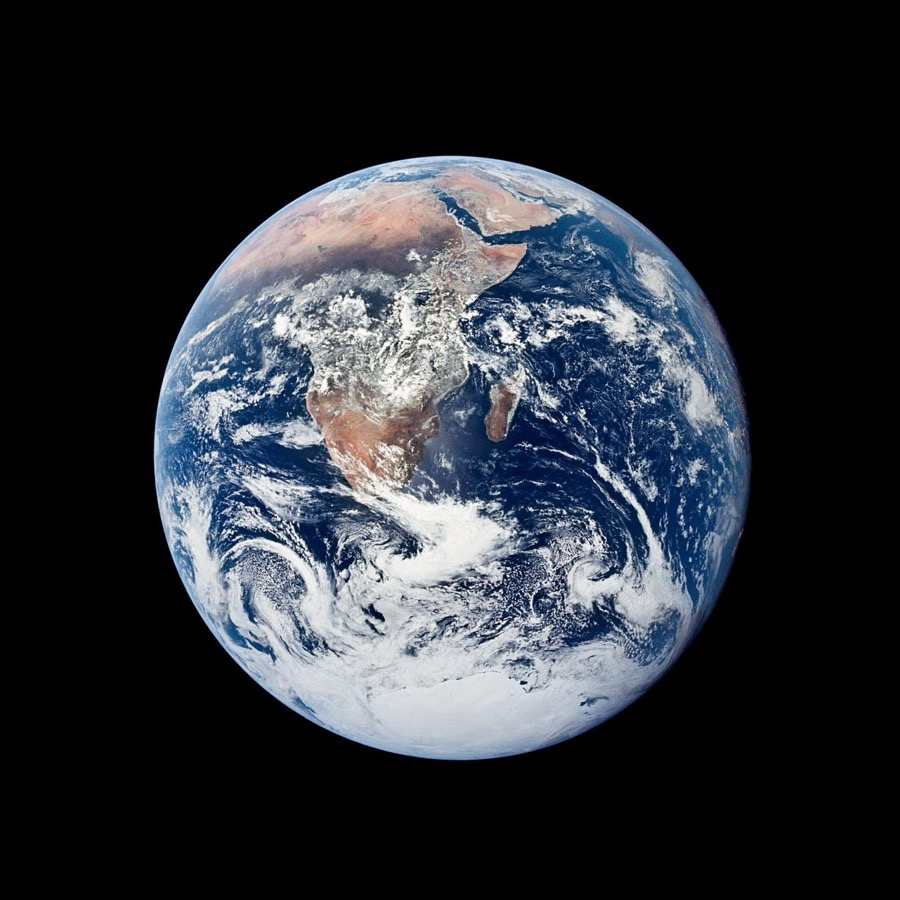
\includegraphics[width=0.55\linewidth]{images/blue-marble-nasa.jpg}
  \caption{Beispielabbildung mit Quellenangabe~\cite{nasa-blue-marble}}
  \label{abb:blue-marble}
\end{figure}

Vektorgrafiken haben gegenüber Screenshots den Vorteil, dass

\begin{itemize}
  \item sie jederzeit editiert werden können,
  \item sie beliebig skaliert werden können, ohne unscharf zu werden,
  \item alle Grafiken einheitlich vergrößert oder verkleinert werden können.
        Das verbessert das Layout ungemein.
\end{itemize}

Abbildungen stehen immer alleinstehend und zentriert. Die Breite wird
relativ zur Textbreite angegeben (\lstinline|width=0.75\linewidth|), damit
sie nie über den Satzspiegel hinausragt. Sollen mehrere Grafiken
nebeneinander stehen, verwendet dafür zwei \lstinline|minipage|-Umgebungen
innerhalb einer \lstinline|figure|.

Die Positionierung übernimmt \LaTeX. Die Angabe \lstinline|[htbp]| erlaubt
es, die Abbildung an die Stelle im Text, an den Seitenanfang, an das
Seitenende oder auf eine eigene Seite zu setzen. Eine Abbildung kann dadurch
auf der Folgeseite landen -- das ist beabsichtigt und kein Fehler.

\subsection{Beschriftungen}

Alle Grafiken und Tabellen sind zu beschriften und mit Quellenangaben zu
versehen. Im Text muss auf jede Abbildung und jede Tabelle Bezug genommen
werden.

Die Beschriftung erfolgt mit \lstinline|\caption| innerhalb der
\lstinline|figure|- bzw.\ \lstinline|table|-Umgebung. Nur so werden
Abbildungs- und Tabellenverzeichnis korrekt geführt. Bei Abbildungen steht
die Beschriftung unter der Grafik, bei Tabellen darüber; die Vorlage stellt
das automatisch richtig ein.

Abbildungen werden mit \enquote{Abb.} und Tabellen mit \enquote{Tab.}
bezeichnet. Auch das erledigt die Vorlage; die Nummerierung läuft
durchgehend und nicht kapitelweise. In englischsprachigen Diplomarbeiten
wird \enquote{Abb.} durch \enquote{Fig.} ersetzt -- dafür genügt die
Klassenoption \lstinline|englisch|.

Unmittelbar nach \lstinline|\caption| gehört ein \lstinline|\label|. Ohne
Label lässt sich die Abbildung später nicht referenzieren. Bewährt hat sich
ein Präfix je Objektart: \lstinline|abb:|, \lstinline|tab:| und
\lstinline|code:|.

\subsection{Querverweise}

Textpassagen, die sich auf andere Kapitel, Grafiken oder Tabellen beziehen,
müssen eine Referenz enthalten. Diese wird mit \lstinline|\ref| erzeugt und
enthält zumindest die Kategorie und die Nummer, also etwa
\lstinline|Abb.~\ref{abb:aufbau}|. Das geschützte Leerzeichen
\lstinline|~| verhindert, dass zwischen Bezeichnung und Nummer umgebrochen
wird.

Liegen referenzierender Text und referenziertes Objekt mehr als eine Seite
auseinander, ist zusätzlich die Seitenzahl mit \lstinline|\pageref|
anzugeben.

Anders als in Word müssen Querverweise und Verzeichnisse nicht manuell
aktualisiert werden. \LaTeX{} löst sie beim Übersetzen auf, benötigt dafür
aber mehrere Durchläufe. \lstinline|latexmk| (bzw.\ \lstinline|make pdf|)
wiederholt den Lauf so lange, bis sich nichts mehr ändert. Meldet das
Protokoll am Ende \enquote{There were undefined references}, fehlt ein
\lstinline|\label| oder es ist falsch geschrieben.

\subsection{Quellenangaben}

In wissenschaftlichen Arbeiten ist es verpflichtend, die Quelle jeder
Aussage anzugeben, die nicht von einem selbst stammt. Der Leser muss die
Möglichkeit haben, die Ausführungen des Autors nachzuprüfen.

Zu diesem Zweck müssen im Text der Diplomarbeit alle verwendeten Quellen
(Fachbücher, Fachzeitschriften, Herstellerunterlagen, Webseiten, \ldots)
angegeben werden. Dies geschieht am Ende des zitierten Textes durch Angabe
der Quelle. Informationen aus Lehrbüchern können als Allgemeinwissen
vorausgesetzt werden und müssen nicht zitiert werden.

Bei inhaltlichen Zitaten, dem Normalfall in technischen Arbeiten, wird der
Inhalt der Quelle nur sinngemäß wiedergegeben.

Bei wörtlichen Zitaten, die in technischen Arbeiten eher selten auftreten,
wird die wörtlich zitierte Textstelle zwischen Anführungszeichen gesetzt,
dahinter steht die Quellenangabe. Eigene Kommentare im Zitat oder
Verkürzungen werden in eckigen Klammern angegeben. Kurze Zitate stehen mit
\lstinline|\zitat| im Fließtext, längere in der Umgebung
\lstinline|zitatfreistehend|.

Beispiel für ein Zitat im Text der Diplomarbeit:
\zitat{[\ldots] kann in diesem Fall eine relationale Datenbank vorteilhaft
eingesetzt werden}~\cite{beispiel-buch}.

Beispiel für ein Zitat als eigener Absatz:

\begin{zitatfreistehend}
  \enquote{The basic guideline for citing online sources is to follow the
  standard citation for the citation, or add the DOI in place of page
  numbers if the source is not paginated.}~\cite{beispiel-artikel}
\end{zitatfreistehend}

Für Diplomarbeiten an der \ac{HTL} Donaustadt ist der IEEE-Zitierstil zu
verwenden. Jeder Quelle wird eine Nummer zugeordnet und in eckigen Klammern
angegeben. Diese Vorlage stellt den Stil bereits ein; zitiert wird mit
\lstinline|\cite{schluessel}|, wobei der Schlüssel aus
\lstinline|references.bib| stammt. Das Quellenverzeichnis wird daraus
automatisch erzeugt und enthält nur tatsächlich zitierte Einträge.

Zum Verwalten der Quellen empfiehlt sich Zotero mit dem Plug-in Better
BibTeX, das \lstinline|references.bib| bei jeder Änderung automatisch neu
exportiert.

Es gibt viele verschiedene Typen von Quellen. Tab.~\ref{tab:quellentypen}
zeigt die häufigsten, den passenden BibTeX-Eintragstyp und die
Informationen, die mindestens enthalten sein sollten.

\begin{table}[htbp]
  \centering
  \caption{Quellentypen}
  \label{tab:quellentypen}
  \begin{tabular}{@{}p{0.28\linewidth}p{0.16\linewidth}p{0.46\linewidth}@{}}
    \toprule
    \tabkopf{Quellentyp} & \tabkopf{Eintragstyp} &
      \tabkopf{wichtigste Informationen} \\
    \midrule
    Buch (auch E-Books, Broschüren) & \lstinline|@book| &
      Autor(en), Titel, Auflage, Verlag, Ort, ISBN \\
    Diplomarbeit, Dissertation & \lstinline|@thesis| &
      Autor(en), Titel, Institution, Ort, Datum \\
    Webseite (auch PDF) & \lstinline|@online| &
      Autor(en), Titel, URL, Abrufdatum (\lstinline|urldate|) \\
    Zeitschriftenartikel & \lstinline|@article| &
      Autor(en), Titel, Publikation, Band, Ausgabe, Seiten, Datum \\
    Verwendung von KI & \lstinline|@online| &
      siehe Anhang und die Vorgaben des Ministeriums~\cite{beispiel-online} \\
    \bottomrule
  \end{tabular}
\end{table}

\subsection{Befehle und Umgebungen}

In Word übernehmen Formatvorlagen das einheitliche Layout. In \LaTeX{}
erfüllen Befehle und Umgebungen dieselbe Aufgabe: Der Text beschreibt, was
etwas \emph{ist}, das Aussehen legt die Dokumentklasse \lstinline|htldon.cls|
zentral fest. Dadurch lässt sich die Formatierung nachträglich an einer
einzigen Stelle ändern.

Die in Tab.~\ref{tab:befehle} aufgeführten Befehle stellen sicher, dass alle
Diplomarbeiten den Richtlinien entsprechen. Sie dürfen nur in begründeten
Ausnahmefällen angepasst werden.

\begin{table}[htbp]
  \centering
  \caption{Befehle und Umgebungen der Vorlage}
  \label{tab:befehle}
  \begin{tabular}{@{}p{0.36\linewidth}p{0.58\linewidth}@{}}
    \toprule
    \tabkopf{Befehl} & \tabkopf{Beschreibung} \\
    \midrule
    \lstinline|\chapter| bis \lstinline|\subsubsection| &
      Kapitelüberschriften mit Dezimalklassifikation. Die ersten drei Ebenen
      erscheinen im Inhaltsverzeichnis, \lstinline|\subsubsection| nicht. \\
    \lstinline|\paragraph| &
      Zwischenüberschrift ohne Nummerierung, nicht im Inhaltsverzeichnis. \\
    \lstinline|\abschnittsautor| &
      Verfasser/in eines Abschnitts, erscheint rechts in der Kopfzeile.
      Format: erster Buchstabe des Vornamens, Punkt, Nachname
      (\enquote{M. Muster}). \\
    \lstinline|\zitat|, \lstinline|zitatfreistehend| &
      Kennzeichnung wörtlicher Zitate im Fließtext bzw.\ als eigener Absatz. \\
    \lstinline|\menue| &
      Menüstrukturen (\menue{Datei / Öffnen}) und Tastatureingaben
      (\menue{Strg + A}). \\
    \lstinline|lstlisting|, \lstinline|\lstinline| &
      Quellcode als eigener Block bzw.\ im Fließtext. \\
    \lstinline|\tabkopf| &
      Kopfzeile einer Tabelle. Der Tabelleninhalt selbst wird von der Klasse
      automatisch auf 10\,pt und linksbündig gestellt. \\
    \lstinline|\ac|, \lstinline|\acp| &
      Abkürzung, beim ersten Auftreten ausgeschrieben, im Plural mit
      \lstinline|\acp|. \\
    \lstinline|\cite|, \lstinline|\ref|, \lstinline|\pageref| &
      Quellenangabe, Querverweis, Seitenverweis. \\
    \bottomrule
  \end{tabular}
\end{table}

Überschriften der Kapitel müssen kurz, präzise und selbsterklärend sein.
Beispiele für unzureichende Überschriften: \enquote{5.3 Aufbau},
\enquote{5.3 Messergebnis}, \enquote{5.3 Beispiel}.

Bei Unterüberschriften gilt:

\begin{itemize}
  \item Es muss mindestens zwei Unterpunkte geben. Ein Abschnitt 3.2.1 darf
        daher nicht existieren, wenn kein 3.2.2 folgt.
  \item Unterpunkte sollten inhaltlich ausreichend gefüllt sein und
        mindestens eine halbe Seite umfassen.
  \item Unterpunkte, die lediglich aus einem einzelnen Satz bestehen, werden
        besser als Aufzählung dargestellt.
\end{itemize}

Für die Darstellung von Quellcode gilt:

\begin{itemize}
  \item Umfang:
        \begin{itemize}
          \item Der vollständige Sourcecode gehört ausschließlich auf das
                elektronische Speichermedium.
          \item Im Dokument selbst sollen nur wesentliche Ausschnitte
                aufgenommen werden.
        \end{itemize}
  \item Formatierung: Schriftart und Schriftgröße gibt die
        \lstinline|lstlisting|-Umgebung vor, der Zeilenabstand ist dort
        einzeilig. Die Sprache wird mit
        \lstinline|[language=Python]| angegeben, damit die
        Syntaxhervorhebung stimmt.
  \item Inhaltliche Anforderungen: Der Sourcecode muss ausreichend
        kommentiert sein.
  \item Verwendung im Fließtext: Wird Sourcecode im Text erwähnt, ist
        \lstinline|\lstinline| zu verwenden. Zusätzliche Anführungszeichen
        sind nicht erforderlich. Beispiel: Mit dem Befehl
        \lstinline|ShowModal| wird ein Frame geöffnet.
\end{itemize}

\section{Beschreibung der Kapitel}

\subsection{Titelseite}

Die Titelseite wird vollständig aus \lstinline|metadata.tex| erzeugt. Dort
sind einzutragen:

\begin{itemize}
  \item der Titel der Diplomarbeit mit \lstinline|\titel|. Er wird
        automatisch in die Kopfzeile übernommen.
  \item ein Projektlogo, Bild oder eine Zeichnung mit
        \lstinline|\projektlogo|.
  \item alle Verfasser/innen mit \lstinline|\teammitglied| und die
        Betreuung mit \lstinline|\betreuung|.
  \item Schuljahr, Abteilung und Klasse.
\end{itemize}

Falls alle Verfasser/innen oder Betreuer/innen dasselbe Geschlecht haben,
kann die geschlechtsspezifische Form verwendet werden; dafür ist das
optionale Argument von \lstinline|\betreuung| vorgesehen.

\subsection{Verfassererklärung}

In der Verfassererklärung bekennen sich die Verfasser/innen zu einem
wissenschaftlichen Arbeitsstil. Sollten im Nachhinein grobe Verstöße dagegen
aufgedeckt werden, kann die Arbeit für ungültig erklärt und der Abschluss
revidiert werden.

Die Erklärung erzeugt \lstinline|\eigenstaendigkeitserklaerung|. Je
Teammitglied entsteht automatisch eine Unterschriftszeile. Zu ergänzen sind
gegebenenfalls Kooperationen mit Firmen und Sperrvermerke.

\subsection{Problemstellung}

Die Seite \enquote{Problemstellung} wird durch den eingescannten Antrag (mit
allen Stempeln und Unterschriften) vollflächig ersetzt. Dazu wird in
\lstinline|frontmatter/problem-statement.tex| das Scan-PDF eingebunden.

\subsection{Kurzfassung bzw.\ Abstract}

Die Kurzfassung bzw.\ der Abstract soll kurz, prägnant und verständlich den
Inhalt der Arbeit wiedergeben: Zielsetzung, Ablauf, wichtigste Erkenntnisse,
wesentliche Merkmale des realisierten Produkts, Schlussfolgerungen und
Ausblick. Beide sind als eigenständiges Dokument zu konzipieren, das
unabhängig von der Diplomarbeit gelesen und verstanden werden kann, und
sollen in Deutsch und Englisch jeweils nicht mehr als eine Seite umfassen.

\subsection{Inhaltsverzeichnis}

Das Inhaltsverzeichnis wird automatisch aus den Überschriften erstellt. Es
zeigt die ersten drei Ebenen, der Text steht linksbündig, die Seitenzahlen
rechtsbündig, als Füllzeichen dienen Punkte. Eine manuelle Aktualisierung
ist nicht nötig.

\subsection{Die weiteren Kapitel}

Die Kapitel Projektplanung, Technische Grundlagen, Praktische Realisierung
sowie Evaluierung und Ergebnisse beschreiben die Diplomarbeit im Detail.

Für die Beurteilung ist es wichtig, den/die Verfasser/in zu kennen. Daher
ist dieser Hinweis auf jeder Seite rechtsbündig in der Kopfzeile zu
vermerken. Dafür wird \lstinline|\abschnittsautor| direkt nach der
Überschrift gesetzt; der Eintrag gilt ab dort bis zur nächsten Angabe.
Haben mehrere Personen gemeinsam an einem Abschnitt gearbeitet, sind alle zu
nennen, durch Komma getrennt:
\lstinline|\abschnittsautor{A. Erste, B. Zweite}|.

Die Projektplanung soll die systematische Durchführung der Diplomarbeit
innerhalb des Projektteams beschreiben. Dabei sollen geplante Ziele und
tatsächlich erreichte Ergebnisse miteinander verglichen und die Unterschiede
reflektiert werden. Beim klassischen Wasserfall-Projektmanagement können
etwa die Meilensteine als Referenz dienen, bei agiler Projektorganisation
die Sprint-Reviews.

Im Kapitel Technische Grundlagen finden sich alle für das unmittelbare
technische Verständnis der Diplomarbeit relevanten Inhalte. Hier wird
insbesondere auf korrekte Zitate und den sorgfältigen Einsatz von Quellen
geachtet.

Das Kapitel Praktische Realisierung enthält die praktischen Eigenleistungen
der Diplomarbeit. Dabei sollen die Vorgänge und Untersuchungen beschrieben
und nachvollziehbar dokumentiert werden.

Im Kapitel Evaluierung und Ergebnisse erfolgt die Darstellung und Bewertung
der abschließenden Arbeit. Hier soll ebenso, sofern vorhanden, das
Endprodukt bzw.\ der Prototyp präsentiert und beschrieben werden.

\subsection{Anhang}

Im Anhang können alle Informationen gesammelt werden, die zwar zur
Diplomarbeit gehören, jedoch im Inhaltsteil den Rahmen gesprengt hätten.
Dazu zählen wichtige Notizen (z.\,B. Gesprächsprotokolle), Normen,
Schnittstellendefinitionen oder Präsentationen. Weiters soll der Anhang den
Inhalt eines beigefügten elektronischen Speichermediums sowie einen
einseitigen Lebenslauf jedes Teammitglieds enthalten.

Verpflichtend ist außerdem die Dokumentation aller eingesetzten KI-basierten
Hilfsmittel. Dafür ist \lstinline|appendix/ai-tools.tex| vorgesehen.

% in diplomarbeit.tex entfernen und diese Datei mitlöschen.
% =====================================================================
\chapter{Richtlinie für das Verfassen von Diplomarbeiten}

Diese Richtlinie beschreibt die formalen und inhaltlichen Anforderungen an
eine wissenschaftliche Publikation und soll ein einheitliches
Erscheinungsbild der Diplomarbeiten sicherstellen. Dieses Kapitel beschreibt
weiters, wie die vorliegende Diplomarbeitsvorlage zu verwenden ist, und ist
im finalen Dokument zu entfernen.

Es sind bewusst nur die wesentlichen Punkte festgelegt. In Absprache mit dem
Betreuer/der Betreuerin soll stets Freiraum für die individuelle Gestaltung
sowie projektbedingte Erfordernisse bleiben.

\section{Allgemein}

Die Diplomarbeit soll kurz und prägnant -- aber vollständig -- gehalten sein
und einen Umfang von ca.\ 70 Seiten (ohne Anhang) bei einer Teamgröße von
2 Personen umfassen. Die inhaltliche Qualität bei in Umfang eingeschränkter
Darstellung ist ein wesentliches Ziel jeder wissenschaftlichen Publikation
und wird auch in die Beurteilung einbezogen. Grafische Darstellungen,
Übersichtstabellen und Diagramme sind wichtige Hilfsmittel, um diese Vorgabe
einhalten zu können.

Einige Tipps:

\begin{itemize}
  \item Das Verwenden der \enquote{ich}- und \enquote{wir}-Form sowie von
        \enquote{man}-Aussagen ist zu vermeiden.
  \item Abkürzungen müssen unmittelbar nach ihrem ersten Auftreten erläutert
        werden; falls erforderlich, ist ein Abkürzungsverzeichnis zu
        erstellen. Der Befehl \lstinline|\ac{API}| erledigt das automatisch:
        beim ersten Auftreten schreibt er die Abkürzung aus, danach nicht
        mehr.
  \item Über Themen, die nur indirekt mit der gestellten Aufgabe zu tun
        haben, soll nicht berichtet werden. Die ausführliche Darstellung von
        Grundlagenwissen ist nicht erforderlich; meistens reicht das Zitieren
        geeigneter Quellen.
  \item Arbeitet im Team über ein Git-Repository und legt pro Kapitel eine
        eigene Datei an. So lassen sich Änderungen nachvollziehen und
        Konflikte auf einzelne Absätze eingrenzen.
\end{itemize}

\subsection{Platzhalter in dieser Vorlage}

Alle Beispieltexte in dieser Vorlage sind zu ersetzen oder zu löschen. Das
betrifft insbesondere:

\begin{itemize}
  \item die Metadaten in \lstinline|metadata.tex| (Titel, Team, Betreuung,
        Schuljahr, Klasse),
  \item die Beispielkapitel in \lstinline|chapters/|,
  \item die Beispielquellen in \lstinline|references.bib|,
  \item das Abkürzungsverzeichnis in \lstinline|diplomarbeit.tex|,
  \item dieses gesamte Kapitel~6.
\end{itemize}

Um dieses Kapitel zu entfernen, genügt es, in \lstinline|diplomarbeit.tex|
die Zeile \lstinline|% =====================================================================
% Kapitel 6 der Abteilungsvorlage, auf LaTeX übertragen.
% Vor der Abgabe komplett löschen: die Zeile % =====================================================================
% Kapitel 6 der Abteilungsvorlage, auf LaTeX übertragen.
% Vor der Abgabe komplett löschen: die Zeile % =====================================================================
% Kapitel 6 der Abteilungsvorlage, auf LaTeX übertragen.
% Vor der Abgabe komplett löschen: die Zeile \input{chapters/06-guideline}
% in diplomarbeit.tex entfernen und diese Datei mitlöschen.
% =====================================================================
\chapter{Richtlinie für das Verfassen von Diplomarbeiten}

Diese Richtlinie beschreibt die formalen und inhaltlichen Anforderungen an
eine wissenschaftliche Publikation und soll ein einheitliches
Erscheinungsbild der Diplomarbeiten sicherstellen. Dieses Kapitel beschreibt
weiters, wie die vorliegende Diplomarbeitsvorlage zu verwenden ist, und ist
im finalen Dokument zu entfernen.

Es sind bewusst nur die wesentlichen Punkte festgelegt. In Absprache mit dem
Betreuer/der Betreuerin soll stets Freiraum für die individuelle Gestaltung
sowie projektbedingte Erfordernisse bleiben.

\section{Allgemein}

Die Diplomarbeit soll kurz und prägnant -- aber vollständig -- gehalten sein
und einen Umfang von ca.\ 70 Seiten (ohne Anhang) bei einer Teamgröße von
2 Personen umfassen. Die inhaltliche Qualität bei in Umfang eingeschränkter
Darstellung ist ein wesentliches Ziel jeder wissenschaftlichen Publikation
und wird auch in die Beurteilung einbezogen. Grafische Darstellungen,
Übersichtstabellen und Diagramme sind wichtige Hilfsmittel, um diese Vorgabe
einhalten zu können.

Einige Tipps:

\begin{itemize}
  \item Das Verwenden der \enquote{ich}- und \enquote{wir}-Form sowie von
        \enquote{man}-Aussagen ist zu vermeiden.
  \item Abkürzungen müssen unmittelbar nach ihrem ersten Auftreten erläutert
        werden; falls erforderlich, ist ein Abkürzungsverzeichnis zu
        erstellen. Der Befehl \lstinline|\ac{API}| erledigt das automatisch:
        beim ersten Auftreten schreibt er die Abkürzung aus, danach nicht
        mehr.
  \item Über Themen, die nur indirekt mit der gestellten Aufgabe zu tun
        haben, soll nicht berichtet werden. Die ausführliche Darstellung von
        Grundlagenwissen ist nicht erforderlich; meistens reicht das Zitieren
        geeigneter Quellen.
  \item Arbeitet im Team über ein Git-Repository und legt pro Kapitel eine
        eigene Datei an. So lassen sich Änderungen nachvollziehen und
        Konflikte auf einzelne Absätze eingrenzen.
\end{itemize}

\subsection{Platzhalter in dieser Vorlage}

Alle Beispieltexte in dieser Vorlage sind zu ersetzen oder zu löschen. Das
betrifft insbesondere:

\begin{itemize}
  \item die Metadaten in \lstinline|metadata.tex| (Titel, Team, Betreuung,
        Schuljahr, Klasse),
  \item die Beispielkapitel in \lstinline|chapters/|,
  \item die Beispielquellen in \lstinline|references.bib|,
  \item das Abkürzungsverzeichnis in \lstinline|diplomarbeit.tex|,
  \item dieses gesamte Kapitel~6.
\end{itemize}

Um dieses Kapitel zu entfernen, genügt es, in \lstinline|diplomarbeit.tex|
die Zeile \lstinline|\input{chapters/06-guideline}| zu löschen. Die Einträge
im Inhaltsverzeichnis und in den übrigen Verzeichnissen verschwinden beim
nächsten Übersetzen von selbst.

\subsection{Abgabe der Diplomarbeit}

Die Diplomarbeit ist in gedruckter bzw.\ gebundener Form und in digitaler
Form vorzulegen. Dem Abteilungsvorstand sind zwei geheftete Exemplare (ein
Belegexemplar und ein Beurteilungsexemplar für den/die Betreuer/in) zu
übergeben.

Nach erfolgter Beurteilung geht das Beurteilungsexemplar temporär zurück an
die Diplomarbeitsgruppe. Nun können letzte Korrekturen (ohne
Beurteilungsrelevanz) vorgenommen werden. Anschließend wird die Arbeit erneut
ausgedruckt und gesammelt zur Bindung außer Haus gegeben. Weitere Exemplare
für Kooperationspartner (Firmen, Institutionen) oder Projektteilnehmer können
in diesem Zusammenhang erstellt werden.

\subsection{Grafiken}

Abbildungen müssen in gut lesbarer Bildqualität eingefügt werden. Grafiken
sollten am besten in einem vektorbasierten Zeichenprogramm (z.\,B. Inkscape,
draw.io) erstellt und als PDF exportiert werden; PDF und PNG lassen sich
direkt einbinden, SVG nicht. Alle Bilddateien gehören in den Ordner
\lstinline|images/|.

\begin{lstlisting}[language={[LaTeX]TeX}, caption={Eine Abbildung einbinden},
                   label=code:abbildung]
\begin{figure}[htbp]
  \centering
  
\includegraphics[width=0.75\linewidth]{images/example-figure.pdf}
  \caption{Aufbau des Systems}
  \label{abb:aufbau}
\end{figure}
\end{lstlisting}

Abb.~\ref{abb:blue-marble} zeigt, wie das Ergebnis aussieht. Stammt die
Grafik nicht von euch selbst, gehört die Quelle in die Beschriftung.

\begin{figure}[htbp]
  \centering
  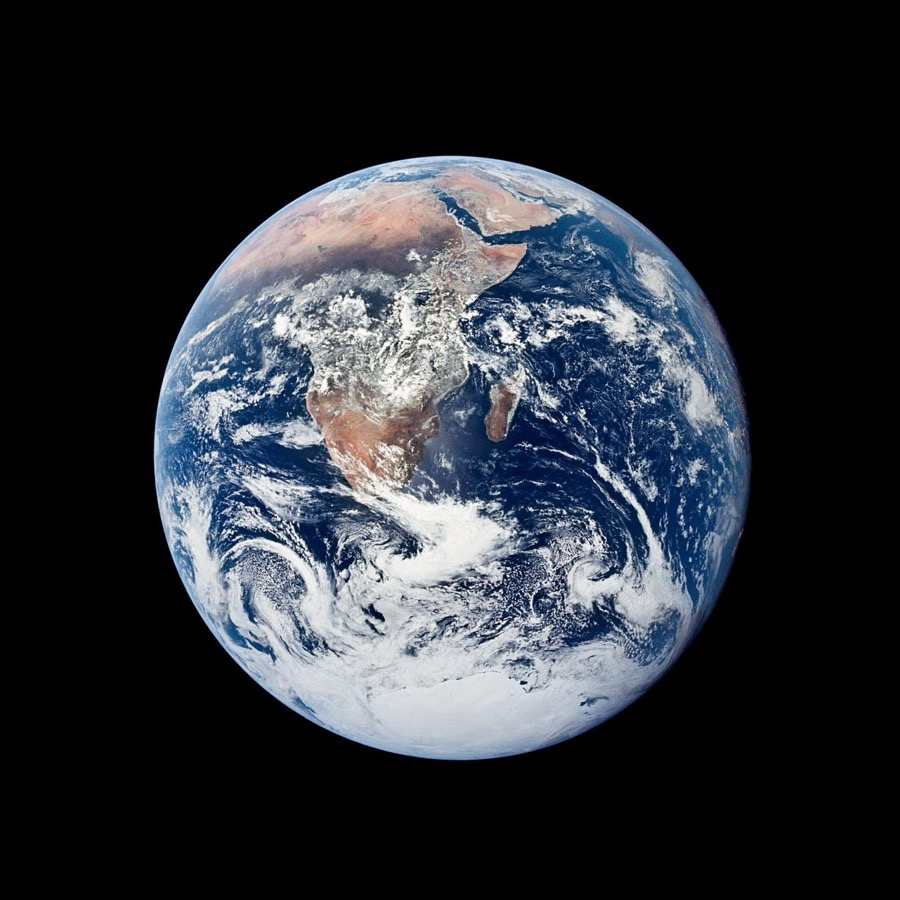
\includegraphics[width=0.55\linewidth]{images/blue-marble-nasa.jpg}
  \caption{Beispielabbildung mit Quellenangabe~\cite{nasa-blue-marble}}
  \label{abb:blue-marble}
\end{figure}

Vektorgrafiken haben gegenüber Screenshots den Vorteil, dass

\begin{itemize}
  \item sie jederzeit editiert werden können,
  \item sie beliebig skaliert werden können, ohne unscharf zu werden,
  \item alle Grafiken einheitlich vergrößert oder verkleinert werden können.
        Das verbessert das Layout ungemein.
\end{itemize}

Abbildungen stehen immer alleinstehend und zentriert. Die Breite wird
relativ zur Textbreite angegeben (\lstinline|width=0.75\linewidth|), damit
sie nie über den Satzspiegel hinausragt. Sollen mehrere Grafiken
nebeneinander stehen, verwendet dafür zwei \lstinline|minipage|-Umgebungen
innerhalb einer \lstinline|figure|.

Die Positionierung übernimmt \LaTeX. Die Angabe \lstinline|[htbp]| erlaubt
es, die Abbildung an die Stelle im Text, an den Seitenanfang, an das
Seitenende oder auf eine eigene Seite zu setzen. Eine Abbildung kann dadurch
auf der Folgeseite landen -- das ist beabsichtigt und kein Fehler.

\subsection{Beschriftungen}

Alle Grafiken und Tabellen sind zu beschriften und mit Quellenangaben zu
versehen. Im Text muss auf jede Abbildung und jede Tabelle Bezug genommen
werden.

Die Beschriftung erfolgt mit \lstinline|\caption| innerhalb der
\lstinline|figure|- bzw.\ \lstinline|table|-Umgebung. Nur so werden
Abbildungs- und Tabellenverzeichnis korrekt geführt. Bei Abbildungen steht
die Beschriftung unter der Grafik, bei Tabellen darüber; die Vorlage stellt
das automatisch richtig ein.

Abbildungen werden mit \enquote{Abb.} und Tabellen mit \enquote{Tab.}
bezeichnet. Auch das erledigt die Vorlage; die Nummerierung läuft
durchgehend und nicht kapitelweise. In englischsprachigen Diplomarbeiten
wird \enquote{Abb.} durch \enquote{Fig.} ersetzt -- dafür genügt die
Klassenoption \lstinline|englisch|.

Unmittelbar nach \lstinline|\caption| gehört ein \lstinline|\label|. Ohne
Label lässt sich die Abbildung später nicht referenzieren. Bewährt hat sich
ein Präfix je Objektart: \lstinline|abb:|, \lstinline|tab:| und
\lstinline|code:|.

\subsection{Querverweise}

Textpassagen, die sich auf andere Kapitel, Grafiken oder Tabellen beziehen,
müssen eine Referenz enthalten. Diese wird mit \lstinline|\ref| erzeugt und
enthält zumindest die Kategorie und die Nummer, also etwa
\lstinline|Abb.~\ref{abb:aufbau}|. Das geschützte Leerzeichen
\lstinline|~| verhindert, dass zwischen Bezeichnung und Nummer umgebrochen
wird.

Liegen referenzierender Text und referenziertes Objekt mehr als eine Seite
auseinander, ist zusätzlich die Seitenzahl mit \lstinline|\pageref|
anzugeben.

Anders als in Word müssen Querverweise und Verzeichnisse nicht manuell
aktualisiert werden. \LaTeX{} löst sie beim Übersetzen auf, benötigt dafür
aber mehrere Durchläufe. \lstinline|latexmk| (bzw.\ \lstinline|make pdf|)
wiederholt den Lauf so lange, bis sich nichts mehr ändert. Meldet das
Protokoll am Ende \enquote{There were undefined references}, fehlt ein
\lstinline|\label| oder es ist falsch geschrieben.

\subsection{Quellenangaben}

In wissenschaftlichen Arbeiten ist es verpflichtend, die Quelle jeder
Aussage anzugeben, die nicht von einem selbst stammt. Der Leser muss die
Möglichkeit haben, die Ausführungen des Autors nachzuprüfen.

Zu diesem Zweck müssen im Text der Diplomarbeit alle verwendeten Quellen
(Fachbücher, Fachzeitschriften, Herstellerunterlagen, Webseiten, \ldots)
angegeben werden. Dies geschieht am Ende des zitierten Textes durch Angabe
der Quelle. Informationen aus Lehrbüchern können als Allgemeinwissen
vorausgesetzt werden und müssen nicht zitiert werden.

Bei inhaltlichen Zitaten, dem Normalfall in technischen Arbeiten, wird der
Inhalt der Quelle nur sinngemäß wiedergegeben.

Bei wörtlichen Zitaten, die in technischen Arbeiten eher selten auftreten,
wird die wörtlich zitierte Textstelle zwischen Anführungszeichen gesetzt,
dahinter steht die Quellenangabe. Eigene Kommentare im Zitat oder
Verkürzungen werden in eckigen Klammern angegeben. Kurze Zitate stehen mit
\lstinline|\zitat| im Fließtext, längere in der Umgebung
\lstinline|zitatfreistehend|.

Beispiel für ein Zitat im Text der Diplomarbeit:
\zitat{[\ldots] kann in diesem Fall eine relationale Datenbank vorteilhaft
eingesetzt werden}~\cite{beispiel-buch}.

Beispiel für ein Zitat als eigener Absatz:

\begin{zitatfreistehend}
  \enquote{The basic guideline for citing online sources is to follow the
  standard citation for the citation, or add the DOI in place of page
  numbers if the source is not paginated.}~\cite{beispiel-artikel}
\end{zitatfreistehend}

Für Diplomarbeiten an der \ac{HTL} Donaustadt ist der IEEE-Zitierstil zu
verwenden. Jeder Quelle wird eine Nummer zugeordnet und in eckigen Klammern
angegeben. Diese Vorlage stellt den Stil bereits ein; zitiert wird mit
\lstinline|\cite{schluessel}|, wobei der Schlüssel aus
\lstinline|references.bib| stammt. Das Quellenverzeichnis wird daraus
automatisch erzeugt und enthält nur tatsächlich zitierte Einträge.

Zum Verwalten der Quellen empfiehlt sich Zotero mit dem Plug-in Better
BibTeX, das \lstinline|references.bib| bei jeder Änderung automatisch neu
exportiert.

Es gibt viele verschiedene Typen von Quellen. Tab.~\ref{tab:quellentypen}
zeigt die häufigsten, den passenden BibTeX-Eintragstyp und die
Informationen, die mindestens enthalten sein sollten.

\begin{table}[htbp]
  \centering
  \caption{Quellentypen}
  \label{tab:quellentypen}
  \begin{tabular}{@{}p{0.28\linewidth}p{0.16\linewidth}p{0.46\linewidth}@{}}
    \toprule
    \tabkopf{Quellentyp} & \tabkopf{Eintragstyp} &
      \tabkopf{wichtigste Informationen} \\
    \midrule
    Buch (auch E-Books, Broschüren) & \lstinline|@book| &
      Autor(en), Titel, Auflage, Verlag, Ort, ISBN \\
    Diplomarbeit, Dissertation & \lstinline|@thesis| &
      Autor(en), Titel, Institution, Ort, Datum \\
    Webseite (auch PDF) & \lstinline|@online| &
      Autor(en), Titel, URL, Abrufdatum (\lstinline|urldate|) \\
    Zeitschriftenartikel & \lstinline|@article| &
      Autor(en), Titel, Publikation, Band, Ausgabe, Seiten, Datum \\
    Verwendung von KI & \lstinline|@online| &
      siehe Anhang und die Vorgaben des Ministeriums~\cite{beispiel-online} \\
    \bottomrule
  \end{tabular}
\end{table}

\subsection{Befehle und Umgebungen}

In Word übernehmen Formatvorlagen das einheitliche Layout. In \LaTeX{}
erfüllen Befehle und Umgebungen dieselbe Aufgabe: Der Text beschreibt, was
etwas \emph{ist}, das Aussehen legt die Dokumentklasse \lstinline|htldon.cls|
zentral fest. Dadurch lässt sich die Formatierung nachträglich an einer
einzigen Stelle ändern.

Die in Tab.~\ref{tab:befehle} aufgeführten Befehle stellen sicher, dass alle
Diplomarbeiten den Richtlinien entsprechen. Sie dürfen nur in begründeten
Ausnahmefällen angepasst werden.

\begin{table}[htbp]
  \centering
  \caption{Befehle und Umgebungen der Vorlage}
  \label{tab:befehle}
  \begin{tabular}{@{}p{0.36\linewidth}p{0.58\linewidth}@{}}
    \toprule
    \tabkopf{Befehl} & \tabkopf{Beschreibung} \\
    \midrule
    \lstinline|\chapter| bis \lstinline|\subsubsection| &
      Kapitelüberschriften mit Dezimalklassifikation. Die ersten drei Ebenen
      erscheinen im Inhaltsverzeichnis, \lstinline|\subsubsection| nicht. \\
    \lstinline|\paragraph| &
      Zwischenüberschrift ohne Nummerierung, nicht im Inhaltsverzeichnis. \\
    \lstinline|\abschnittsautor| &
      Verfasser/in eines Abschnitts, erscheint rechts in der Kopfzeile.
      Format: erster Buchstabe des Vornamens, Punkt, Nachname
      (\enquote{M. Muster}). \\
    \lstinline|\zitat|, \lstinline|zitatfreistehend| &
      Kennzeichnung wörtlicher Zitate im Fließtext bzw.\ als eigener Absatz. \\
    \lstinline|\menue| &
      Menüstrukturen (\menue{Datei / Öffnen}) und Tastatureingaben
      (\menue{Strg + A}). \\
    \lstinline|lstlisting|, \lstinline|\lstinline| &
      Quellcode als eigener Block bzw.\ im Fließtext. \\
    \lstinline|\tabkopf| &
      Kopfzeile einer Tabelle. Der Tabelleninhalt selbst wird von der Klasse
      automatisch auf 10\,pt und linksbündig gestellt. \\
    \lstinline|\ac|, \lstinline|\acp| &
      Abkürzung, beim ersten Auftreten ausgeschrieben, im Plural mit
      \lstinline|\acp|. \\
    \lstinline|\cite|, \lstinline|\ref|, \lstinline|\pageref| &
      Quellenangabe, Querverweis, Seitenverweis. \\
    \bottomrule
  \end{tabular}
\end{table}

Überschriften der Kapitel müssen kurz, präzise und selbsterklärend sein.
Beispiele für unzureichende Überschriften: \enquote{5.3 Aufbau},
\enquote{5.3 Messergebnis}, \enquote{5.3 Beispiel}.

Bei Unterüberschriften gilt:

\begin{itemize}
  \item Es muss mindestens zwei Unterpunkte geben. Ein Abschnitt 3.2.1 darf
        daher nicht existieren, wenn kein 3.2.2 folgt.
  \item Unterpunkte sollten inhaltlich ausreichend gefüllt sein und
        mindestens eine halbe Seite umfassen.
  \item Unterpunkte, die lediglich aus einem einzelnen Satz bestehen, werden
        besser als Aufzählung dargestellt.
\end{itemize}

Für die Darstellung von Quellcode gilt:

\begin{itemize}
  \item Umfang:
        \begin{itemize}
          \item Der vollständige Sourcecode gehört ausschließlich auf das
                elektronische Speichermedium.
          \item Im Dokument selbst sollen nur wesentliche Ausschnitte
                aufgenommen werden.
        \end{itemize}
  \item Formatierung: Schriftart und Schriftgröße gibt die
        \lstinline|lstlisting|-Umgebung vor, der Zeilenabstand ist dort
        einzeilig. Die Sprache wird mit
        \lstinline|[language=Python]| angegeben, damit die
        Syntaxhervorhebung stimmt.
  \item Inhaltliche Anforderungen: Der Sourcecode muss ausreichend
        kommentiert sein.
  \item Verwendung im Fließtext: Wird Sourcecode im Text erwähnt, ist
        \lstinline|\lstinline| zu verwenden. Zusätzliche Anführungszeichen
        sind nicht erforderlich. Beispiel: Mit dem Befehl
        \lstinline|ShowModal| wird ein Frame geöffnet.
\end{itemize}

\section{Beschreibung der Kapitel}

\subsection{Titelseite}

Die Titelseite wird vollständig aus \lstinline|metadata.tex| erzeugt. Dort
sind einzutragen:

\begin{itemize}
  \item der Titel der Diplomarbeit mit \lstinline|\titel|. Er wird
        automatisch in die Kopfzeile übernommen.
  \item ein Projektlogo, Bild oder eine Zeichnung mit
        \lstinline|\projektlogo|.
  \item alle Verfasser/innen mit \lstinline|\teammitglied| und die
        Betreuung mit \lstinline|\betreuung|.
  \item Schuljahr, Abteilung und Klasse.
\end{itemize}

Falls alle Verfasser/innen oder Betreuer/innen dasselbe Geschlecht haben,
kann die geschlechtsspezifische Form verwendet werden; dafür ist das
optionale Argument von \lstinline|\betreuung| vorgesehen.

\subsection{Verfassererklärung}

In der Verfassererklärung bekennen sich die Verfasser/innen zu einem
wissenschaftlichen Arbeitsstil. Sollten im Nachhinein grobe Verstöße dagegen
aufgedeckt werden, kann die Arbeit für ungültig erklärt und der Abschluss
revidiert werden.

Die Erklärung erzeugt \lstinline|\eigenstaendigkeitserklaerung|. Je
Teammitglied entsteht automatisch eine Unterschriftszeile. Zu ergänzen sind
gegebenenfalls Kooperationen mit Firmen und Sperrvermerke.

\subsection{Problemstellung}

Die Seite \enquote{Problemstellung} wird durch den eingescannten Antrag (mit
allen Stempeln und Unterschriften) vollflächig ersetzt. Dazu wird in
\lstinline|frontmatter/problem-statement.tex| das Scan-PDF eingebunden.

\subsection{Kurzfassung bzw.\ Abstract}

Die Kurzfassung bzw.\ der Abstract soll kurz, prägnant und verständlich den
Inhalt der Arbeit wiedergeben: Zielsetzung, Ablauf, wichtigste Erkenntnisse,
wesentliche Merkmale des realisierten Produkts, Schlussfolgerungen und
Ausblick. Beide sind als eigenständiges Dokument zu konzipieren, das
unabhängig von der Diplomarbeit gelesen und verstanden werden kann, und
sollen in Deutsch und Englisch jeweils nicht mehr als eine Seite umfassen.

\subsection{Inhaltsverzeichnis}

Das Inhaltsverzeichnis wird automatisch aus den Überschriften erstellt. Es
zeigt die ersten drei Ebenen, der Text steht linksbündig, die Seitenzahlen
rechtsbündig, als Füllzeichen dienen Punkte. Eine manuelle Aktualisierung
ist nicht nötig.

\subsection{Die weiteren Kapitel}

Die Kapitel Projektplanung, Technische Grundlagen, Praktische Realisierung
sowie Evaluierung und Ergebnisse beschreiben die Diplomarbeit im Detail.

Für die Beurteilung ist es wichtig, den/die Verfasser/in zu kennen. Daher
ist dieser Hinweis auf jeder Seite rechtsbündig in der Kopfzeile zu
vermerken. Dafür wird \lstinline|\abschnittsautor| direkt nach der
Überschrift gesetzt; der Eintrag gilt ab dort bis zur nächsten Angabe.
Haben mehrere Personen gemeinsam an einem Abschnitt gearbeitet, sind alle zu
nennen, durch Komma getrennt:
\lstinline|\abschnittsautor{A. Erste, B. Zweite}|.

Die Projektplanung soll die systematische Durchführung der Diplomarbeit
innerhalb des Projektteams beschreiben. Dabei sollen geplante Ziele und
tatsächlich erreichte Ergebnisse miteinander verglichen und die Unterschiede
reflektiert werden. Beim klassischen Wasserfall-Projektmanagement können
etwa die Meilensteine als Referenz dienen, bei agiler Projektorganisation
die Sprint-Reviews.

Im Kapitel Technische Grundlagen finden sich alle für das unmittelbare
technische Verständnis der Diplomarbeit relevanten Inhalte. Hier wird
insbesondere auf korrekte Zitate und den sorgfältigen Einsatz von Quellen
geachtet.

Das Kapitel Praktische Realisierung enthält die praktischen Eigenleistungen
der Diplomarbeit. Dabei sollen die Vorgänge und Untersuchungen beschrieben
und nachvollziehbar dokumentiert werden.

Im Kapitel Evaluierung und Ergebnisse erfolgt die Darstellung und Bewertung
der abschließenden Arbeit. Hier soll ebenso, sofern vorhanden, das
Endprodukt bzw.\ der Prototyp präsentiert und beschrieben werden.

\subsection{Anhang}

Im Anhang können alle Informationen gesammelt werden, die zwar zur
Diplomarbeit gehören, jedoch im Inhaltsteil den Rahmen gesprengt hätten.
Dazu zählen wichtige Notizen (z.\,B. Gesprächsprotokolle), Normen,
Schnittstellendefinitionen oder Präsentationen. Weiters soll der Anhang den
Inhalt eines beigefügten elektronischen Speichermediums sowie einen
einseitigen Lebenslauf jedes Teammitglieds enthalten.

Verpflichtend ist außerdem die Dokumentation aller eingesetzten KI-basierten
Hilfsmittel. Dafür ist \lstinline|appendix/ai-tools.tex| vorgesehen.

% in diplomarbeit.tex entfernen und diese Datei mitlöschen.
% =====================================================================
\chapter{Richtlinie für das Verfassen von Diplomarbeiten}

Diese Richtlinie beschreibt die formalen und inhaltlichen Anforderungen an
eine wissenschaftliche Publikation und soll ein einheitliches
Erscheinungsbild der Diplomarbeiten sicherstellen. Dieses Kapitel beschreibt
weiters, wie die vorliegende Diplomarbeitsvorlage zu verwenden ist, und ist
im finalen Dokument zu entfernen.

Es sind bewusst nur die wesentlichen Punkte festgelegt. In Absprache mit dem
Betreuer/der Betreuerin soll stets Freiraum für die individuelle Gestaltung
sowie projektbedingte Erfordernisse bleiben.

\section{Allgemein}

Die Diplomarbeit soll kurz und prägnant -- aber vollständig -- gehalten sein
und einen Umfang von ca.\ 70 Seiten (ohne Anhang) bei einer Teamgröße von
2 Personen umfassen. Die inhaltliche Qualität bei in Umfang eingeschränkter
Darstellung ist ein wesentliches Ziel jeder wissenschaftlichen Publikation
und wird auch in die Beurteilung einbezogen. Grafische Darstellungen,
Übersichtstabellen und Diagramme sind wichtige Hilfsmittel, um diese Vorgabe
einhalten zu können.

Einige Tipps:

\begin{itemize}
  \item Das Verwenden der \enquote{ich}- und \enquote{wir}-Form sowie von
        \enquote{man}-Aussagen ist zu vermeiden.
  \item Abkürzungen müssen unmittelbar nach ihrem ersten Auftreten erläutert
        werden; falls erforderlich, ist ein Abkürzungsverzeichnis zu
        erstellen. Der Befehl \lstinline|\ac{API}| erledigt das automatisch:
        beim ersten Auftreten schreibt er die Abkürzung aus, danach nicht
        mehr.
  \item Über Themen, die nur indirekt mit der gestellten Aufgabe zu tun
        haben, soll nicht berichtet werden. Die ausführliche Darstellung von
        Grundlagenwissen ist nicht erforderlich; meistens reicht das Zitieren
        geeigneter Quellen.
  \item Arbeitet im Team über ein Git-Repository und legt pro Kapitel eine
        eigene Datei an. So lassen sich Änderungen nachvollziehen und
        Konflikte auf einzelne Absätze eingrenzen.
\end{itemize}

\subsection{Platzhalter in dieser Vorlage}

Alle Beispieltexte in dieser Vorlage sind zu ersetzen oder zu löschen. Das
betrifft insbesondere:

\begin{itemize}
  \item die Metadaten in \lstinline|metadata.tex| (Titel, Team, Betreuung,
        Schuljahr, Klasse),
  \item die Beispielkapitel in \lstinline|chapters/|,
  \item die Beispielquellen in \lstinline|references.bib|,
  \item das Abkürzungsverzeichnis in \lstinline|diplomarbeit.tex|,
  \item dieses gesamte Kapitel~6.
\end{itemize}

Um dieses Kapitel zu entfernen, genügt es, in \lstinline|diplomarbeit.tex|
die Zeile \lstinline|% =====================================================================
% Kapitel 6 der Abteilungsvorlage, auf LaTeX übertragen.
% Vor der Abgabe komplett löschen: die Zeile \input{chapters/06-guideline}
% in diplomarbeit.tex entfernen und diese Datei mitlöschen.
% =====================================================================
\chapter{Richtlinie für das Verfassen von Diplomarbeiten}

Diese Richtlinie beschreibt die formalen und inhaltlichen Anforderungen an
eine wissenschaftliche Publikation und soll ein einheitliches
Erscheinungsbild der Diplomarbeiten sicherstellen. Dieses Kapitel beschreibt
weiters, wie die vorliegende Diplomarbeitsvorlage zu verwenden ist, und ist
im finalen Dokument zu entfernen.

Es sind bewusst nur die wesentlichen Punkte festgelegt. In Absprache mit dem
Betreuer/der Betreuerin soll stets Freiraum für die individuelle Gestaltung
sowie projektbedingte Erfordernisse bleiben.

\section{Allgemein}

Die Diplomarbeit soll kurz und prägnant -- aber vollständig -- gehalten sein
und einen Umfang von ca.\ 70 Seiten (ohne Anhang) bei einer Teamgröße von
2 Personen umfassen. Die inhaltliche Qualität bei in Umfang eingeschränkter
Darstellung ist ein wesentliches Ziel jeder wissenschaftlichen Publikation
und wird auch in die Beurteilung einbezogen. Grafische Darstellungen,
Übersichtstabellen und Diagramme sind wichtige Hilfsmittel, um diese Vorgabe
einhalten zu können.

Einige Tipps:

\begin{itemize}
  \item Das Verwenden der \enquote{ich}- und \enquote{wir}-Form sowie von
        \enquote{man}-Aussagen ist zu vermeiden.
  \item Abkürzungen müssen unmittelbar nach ihrem ersten Auftreten erläutert
        werden; falls erforderlich, ist ein Abkürzungsverzeichnis zu
        erstellen. Der Befehl \lstinline|\ac{API}| erledigt das automatisch:
        beim ersten Auftreten schreibt er die Abkürzung aus, danach nicht
        mehr.
  \item Über Themen, die nur indirekt mit der gestellten Aufgabe zu tun
        haben, soll nicht berichtet werden. Die ausführliche Darstellung von
        Grundlagenwissen ist nicht erforderlich; meistens reicht das Zitieren
        geeigneter Quellen.
  \item Arbeitet im Team über ein Git-Repository und legt pro Kapitel eine
        eigene Datei an. So lassen sich Änderungen nachvollziehen und
        Konflikte auf einzelne Absätze eingrenzen.
\end{itemize}

\subsection{Platzhalter in dieser Vorlage}

Alle Beispieltexte in dieser Vorlage sind zu ersetzen oder zu löschen. Das
betrifft insbesondere:

\begin{itemize}
  \item die Metadaten in \lstinline|metadata.tex| (Titel, Team, Betreuung,
        Schuljahr, Klasse),
  \item die Beispielkapitel in \lstinline|chapters/|,
  \item die Beispielquellen in \lstinline|references.bib|,
  \item das Abkürzungsverzeichnis in \lstinline|diplomarbeit.tex|,
  \item dieses gesamte Kapitel~6.
\end{itemize}

Um dieses Kapitel zu entfernen, genügt es, in \lstinline|diplomarbeit.tex|
die Zeile \lstinline|\input{chapters/06-guideline}| zu löschen. Die Einträge
im Inhaltsverzeichnis und in den übrigen Verzeichnissen verschwinden beim
nächsten Übersetzen von selbst.

\subsection{Abgabe der Diplomarbeit}

Die Diplomarbeit ist in gedruckter bzw.\ gebundener Form und in digitaler
Form vorzulegen. Dem Abteilungsvorstand sind zwei geheftete Exemplare (ein
Belegexemplar und ein Beurteilungsexemplar für den/die Betreuer/in) zu
übergeben.

Nach erfolgter Beurteilung geht das Beurteilungsexemplar temporär zurück an
die Diplomarbeitsgruppe. Nun können letzte Korrekturen (ohne
Beurteilungsrelevanz) vorgenommen werden. Anschließend wird die Arbeit erneut
ausgedruckt und gesammelt zur Bindung außer Haus gegeben. Weitere Exemplare
für Kooperationspartner (Firmen, Institutionen) oder Projektteilnehmer können
in diesem Zusammenhang erstellt werden.

\subsection{Grafiken}

Abbildungen müssen in gut lesbarer Bildqualität eingefügt werden. Grafiken
sollten am besten in einem vektorbasierten Zeichenprogramm (z.\,B. Inkscape,
draw.io) erstellt und als PDF exportiert werden; PDF und PNG lassen sich
direkt einbinden, SVG nicht. Alle Bilddateien gehören in den Ordner
\lstinline|images/|.

\begin{lstlisting}[language={[LaTeX]TeX}, caption={Eine Abbildung einbinden},
                   label=code:abbildung]
\begin{figure}[htbp]
  \centering
  
\includegraphics[width=0.75\linewidth]{images/example-figure.pdf}
  \caption{Aufbau des Systems}
  \label{abb:aufbau}
\end{figure}
\end{lstlisting}

Abb.~\ref{abb:blue-marble} zeigt, wie das Ergebnis aussieht. Stammt die
Grafik nicht von euch selbst, gehört die Quelle in die Beschriftung.

\begin{figure}[htbp]
  \centering
  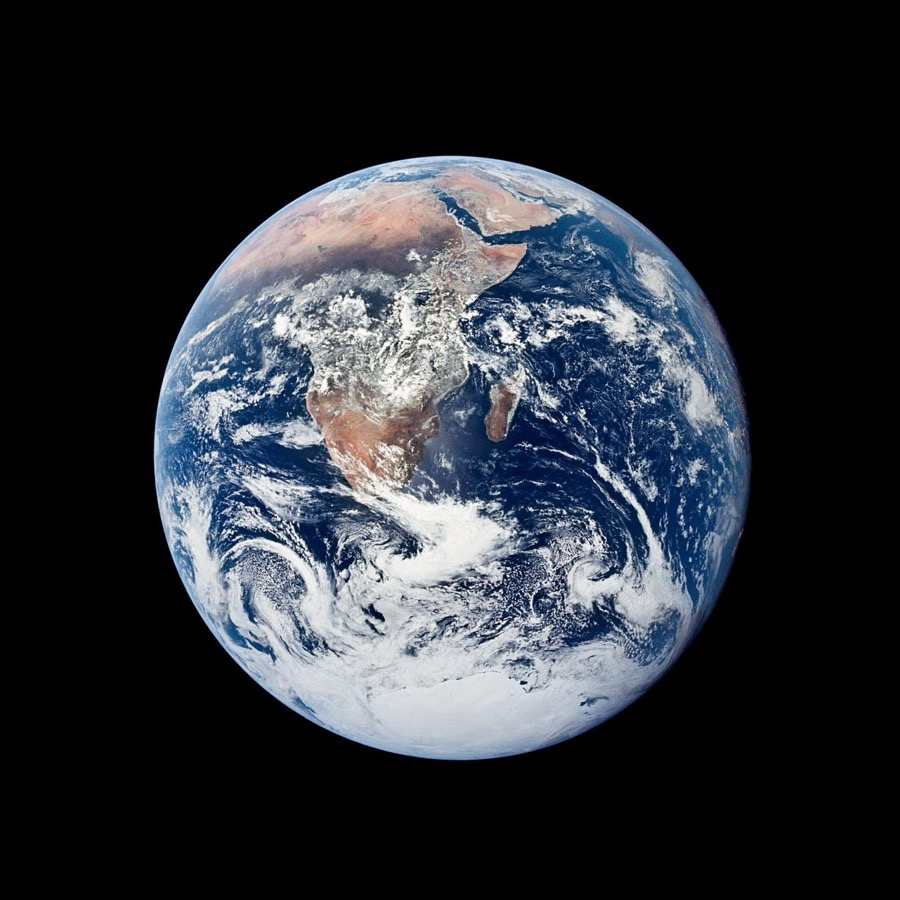
\includegraphics[width=0.55\linewidth]{images/blue-marble-nasa.jpg}
  \caption{Beispielabbildung mit Quellenangabe~\cite{nasa-blue-marble}}
  \label{abb:blue-marble}
\end{figure}

Vektorgrafiken haben gegenüber Screenshots den Vorteil, dass

\begin{itemize}
  \item sie jederzeit editiert werden können,
  \item sie beliebig skaliert werden können, ohne unscharf zu werden,
  \item alle Grafiken einheitlich vergrößert oder verkleinert werden können.
        Das verbessert das Layout ungemein.
\end{itemize}

Abbildungen stehen immer alleinstehend und zentriert. Die Breite wird
relativ zur Textbreite angegeben (\lstinline|width=0.75\linewidth|), damit
sie nie über den Satzspiegel hinausragt. Sollen mehrere Grafiken
nebeneinander stehen, verwendet dafür zwei \lstinline|minipage|-Umgebungen
innerhalb einer \lstinline|figure|.

Die Positionierung übernimmt \LaTeX. Die Angabe \lstinline|[htbp]| erlaubt
es, die Abbildung an die Stelle im Text, an den Seitenanfang, an das
Seitenende oder auf eine eigene Seite zu setzen. Eine Abbildung kann dadurch
auf der Folgeseite landen -- das ist beabsichtigt und kein Fehler.

\subsection{Beschriftungen}

Alle Grafiken und Tabellen sind zu beschriften und mit Quellenangaben zu
versehen. Im Text muss auf jede Abbildung und jede Tabelle Bezug genommen
werden.

Die Beschriftung erfolgt mit \lstinline|\caption| innerhalb der
\lstinline|figure|- bzw.\ \lstinline|table|-Umgebung. Nur so werden
Abbildungs- und Tabellenverzeichnis korrekt geführt. Bei Abbildungen steht
die Beschriftung unter der Grafik, bei Tabellen darüber; die Vorlage stellt
das automatisch richtig ein.

Abbildungen werden mit \enquote{Abb.} und Tabellen mit \enquote{Tab.}
bezeichnet. Auch das erledigt die Vorlage; die Nummerierung läuft
durchgehend und nicht kapitelweise. In englischsprachigen Diplomarbeiten
wird \enquote{Abb.} durch \enquote{Fig.} ersetzt -- dafür genügt die
Klassenoption \lstinline|englisch|.

Unmittelbar nach \lstinline|\caption| gehört ein \lstinline|\label|. Ohne
Label lässt sich die Abbildung später nicht referenzieren. Bewährt hat sich
ein Präfix je Objektart: \lstinline|abb:|, \lstinline|tab:| und
\lstinline|code:|.

\subsection{Querverweise}

Textpassagen, die sich auf andere Kapitel, Grafiken oder Tabellen beziehen,
müssen eine Referenz enthalten. Diese wird mit \lstinline|\ref| erzeugt und
enthält zumindest die Kategorie und die Nummer, also etwa
\lstinline|Abb.~\ref{abb:aufbau}|. Das geschützte Leerzeichen
\lstinline|~| verhindert, dass zwischen Bezeichnung und Nummer umgebrochen
wird.

Liegen referenzierender Text und referenziertes Objekt mehr als eine Seite
auseinander, ist zusätzlich die Seitenzahl mit \lstinline|\pageref|
anzugeben.

Anders als in Word müssen Querverweise und Verzeichnisse nicht manuell
aktualisiert werden. \LaTeX{} löst sie beim Übersetzen auf, benötigt dafür
aber mehrere Durchläufe. \lstinline|latexmk| (bzw.\ \lstinline|make pdf|)
wiederholt den Lauf so lange, bis sich nichts mehr ändert. Meldet das
Protokoll am Ende \enquote{There were undefined references}, fehlt ein
\lstinline|\label| oder es ist falsch geschrieben.

\subsection{Quellenangaben}

In wissenschaftlichen Arbeiten ist es verpflichtend, die Quelle jeder
Aussage anzugeben, die nicht von einem selbst stammt. Der Leser muss die
Möglichkeit haben, die Ausführungen des Autors nachzuprüfen.

Zu diesem Zweck müssen im Text der Diplomarbeit alle verwendeten Quellen
(Fachbücher, Fachzeitschriften, Herstellerunterlagen, Webseiten, \ldots)
angegeben werden. Dies geschieht am Ende des zitierten Textes durch Angabe
der Quelle. Informationen aus Lehrbüchern können als Allgemeinwissen
vorausgesetzt werden und müssen nicht zitiert werden.

Bei inhaltlichen Zitaten, dem Normalfall in technischen Arbeiten, wird der
Inhalt der Quelle nur sinngemäß wiedergegeben.

Bei wörtlichen Zitaten, die in technischen Arbeiten eher selten auftreten,
wird die wörtlich zitierte Textstelle zwischen Anführungszeichen gesetzt,
dahinter steht die Quellenangabe. Eigene Kommentare im Zitat oder
Verkürzungen werden in eckigen Klammern angegeben. Kurze Zitate stehen mit
\lstinline|\zitat| im Fließtext, längere in der Umgebung
\lstinline|zitatfreistehend|.

Beispiel für ein Zitat im Text der Diplomarbeit:
\zitat{[\ldots] kann in diesem Fall eine relationale Datenbank vorteilhaft
eingesetzt werden}~\cite{beispiel-buch}.

Beispiel für ein Zitat als eigener Absatz:

\begin{zitatfreistehend}
  \enquote{The basic guideline for citing online sources is to follow the
  standard citation for the citation, or add the DOI in place of page
  numbers if the source is not paginated.}~\cite{beispiel-artikel}
\end{zitatfreistehend}

Für Diplomarbeiten an der \ac{HTL} Donaustadt ist der IEEE-Zitierstil zu
verwenden. Jeder Quelle wird eine Nummer zugeordnet und in eckigen Klammern
angegeben. Diese Vorlage stellt den Stil bereits ein; zitiert wird mit
\lstinline|\cite{schluessel}|, wobei der Schlüssel aus
\lstinline|references.bib| stammt. Das Quellenverzeichnis wird daraus
automatisch erzeugt und enthält nur tatsächlich zitierte Einträge.

Zum Verwalten der Quellen empfiehlt sich Zotero mit dem Plug-in Better
BibTeX, das \lstinline|references.bib| bei jeder Änderung automatisch neu
exportiert.

Es gibt viele verschiedene Typen von Quellen. Tab.~\ref{tab:quellentypen}
zeigt die häufigsten, den passenden BibTeX-Eintragstyp und die
Informationen, die mindestens enthalten sein sollten.

\begin{table}[htbp]
  \centering
  \caption{Quellentypen}
  \label{tab:quellentypen}
  \begin{tabular}{@{}p{0.28\linewidth}p{0.16\linewidth}p{0.46\linewidth}@{}}
    \toprule
    \tabkopf{Quellentyp} & \tabkopf{Eintragstyp} &
      \tabkopf{wichtigste Informationen} \\
    \midrule
    Buch (auch E-Books, Broschüren) & \lstinline|@book| &
      Autor(en), Titel, Auflage, Verlag, Ort, ISBN \\
    Diplomarbeit, Dissertation & \lstinline|@thesis| &
      Autor(en), Titel, Institution, Ort, Datum \\
    Webseite (auch PDF) & \lstinline|@online| &
      Autor(en), Titel, URL, Abrufdatum (\lstinline|urldate|) \\
    Zeitschriftenartikel & \lstinline|@article| &
      Autor(en), Titel, Publikation, Band, Ausgabe, Seiten, Datum \\
    Verwendung von KI & \lstinline|@online| &
      siehe Anhang und die Vorgaben des Ministeriums~\cite{beispiel-online} \\
    \bottomrule
  \end{tabular}
\end{table}

\subsection{Befehle und Umgebungen}

In Word übernehmen Formatvorlagen das einheitliche Layout. In \LaTeX{}
erfüllen Befehle und Umgebungen dieselbe Aufgabe: Der Text beschreibt, was
etwas \emph{ist}, das Aussehen legt die Dokumentklasse \lstinline|htldon.cls|
zentral fest. Dadurch lässt sich die Formatierung nachträglich an einer
einzigen Stelle ändern.

Die in Tab.~\ref{tab:befehle} aufgeführten Befehle stellen sicher, dass alle
Diplomarbeiten den Richtlinien entsprechen. Sie dürfen nur in begründeten
Ausnahmefällen angepasst werden.

\begin{table}[htbp]
  \centering
  \caption{Befehle und Umgebungen der Vorlage}
  \label{tab:befehle}
  \begin{tabular}{@{}p{0.36\linewidth}p{0.58\linewidth}@{}}
    \toprule
    \tabkopf{Befehl} & \tabkopf{Beschreibung} \\
    \midrule
    \lstinline|\chapter| bis \lstinline|\subsubsection| &
      Kapitelüberschriften mit Dezimalklassifikation. Die ersten drei Ebenen
      erscheinen im Inhaltsverzeichnis, \lstinline|\subsubsection| nicht. \\
    \lstinline|\paragraph| &
      Zwischenüberschrift ohne Nummerierung, nicht im Inhaltsverzeichnis. \\
    \lstinline|\abschnittsautor| &
      Verfasser/in eines Abschnitts, erscheint rechts in der Kopfzeile.
      Format: erster Buchstabe des Vornamens, Punkt, Nachname
      (\enquote{M. Muster}). \\
    \lstinline|\zitat|, \lstinline|zitatfreistehend| &
      Kennzeichnung wörtlicher Zitate im Fließtext bzw.\ als eigener Absatz. \\
    \lstinline|\menue| &
      Menüstrukturen (\menue{Datei / Öffnen}) und Tastatureingaben
      (\menue{Strg + A}). \\
    \lstinline|lstlisting|, \lstinline|\lstinline| &
      Quellcode als eigener Block bzw.\ im Fließtext. \\
    \lstinline|\tabkopf| &
      Kopfzeile einer Tabelle. Der Tabelleninhalt selbst wird von der Klasse
      automatisch auf 10\,pt und linksbündig gestellt. \\
    \lstinline|\ac|, \lstinline|\acp| &
      Abkürzung, beim ersten Auftreten ausgeschrieben, im Plural mit
      \lstinline|\acp|. \\
    \lstinline|\cite|, \lstinline|\ref|, \lstinline|\pageref| &
      Quellenangabe, Querverweis, Seitenverweis. \\
    \bottomrule
  \end{tabular}
\end{table}

Überschriften der Kapitel müssen kurz, präzise und selbsterklärend sein.
Beispiele für unzureichende Überschriften: \enquote{5.3 Aufbau},
\enquote{5.3 Messergebnis}, \enquote{5.3 Beispiel}.

Bei Unterüberschriften gilt:

\begin{itemize}
  \item Es muss mindestens zwei Unterpunkte geben. Ein Abschnitt 3.2.1 darf
        daher nicht existieren, wenn kein 3.2.2 folgt.
  \item Unterpunkte sollten inhaltlich ausreichend gefüllt sein und
        mindestens eine halbe Seite umfassen.
  \item Unterpunkte, die lediglich aus einem einzelnen Satz bestehen, werden
        besser als Aufzählung dargestellt.
\end{itemize}

Für die Darstellung von Quellcode gilt:

\begin{itemize}
  \item Umfang:
        \begin{itemize}
          \item Der vollständige Sourcecode gehört ausschließlich auf das
                elektronische Speichermedium.
          \item Im Dokument selbst sollen nur wesentliche Ausschnitte
                aufgenommen werden.
        \end{itemize}
  \item Formatierung: Schriftart und Schriftgröße gibt die
        \lstinline|lstlisting|-Umgebung vor, der Zeilenabstand ist dort
        einzeilig. Die Sprache wird mit
        \lstinline|[language=Python]| angegeben, damit die
        Syntaxhervorhebung stimmt.
  \item Inhaltliche Anforderungen: Der Sourcecode muss ausreichend
        kommentiert sein.
  \item Verwendung im Fließtext: Wird Sourcecode im Text erwähnt, ist
        \lstinline|\lstinline| zu verwenden. Zusätzliche Anführungszeichen
        sind nicht erforderlich. Beispiel: Mit dem Befehl
        \lstinline|ShowModal| wird ein Frame geöffnet.
\end{itemize}

\section{Beschreibung der Kapitel}

\subsection{Titelseite}

Die Titelseite wird vollständig aus \lstinline|metadata.tex| erzeugt. Dort
sind einzutragen:

\begin{itemize}
  \item der Titel der Diplomarbeit mit \lstinline|\titel|. Er wird
        automatisch in die Kopfzeile übernommen.
  \item ein Projektlogo, Bild oder eine Zeichnung mit
        \lstinline|\projektlogo|.
  \item alle Verfasser/innen mit \lstinline|\teammitglied| und die
        Betreuung mit \lstinline|\betreuung|.
  \item Schuljahr, Abteilung und Klasse.
\end{itemize}

Falls alle Verfasser/innen oder Betreuer/innen dasselbe Geschlecht haben,
kann die geschlechtsspezifische Form verwendet werden; dafür ist das
optionale Argument von \lstinline|\betreuung| vorgesehen.

\subsection{Verfassererklärung}

In der Verfassererklärung bekennen sich die Verfasser/innen zu einem
wissenschaftlichen Arbeitsstil. Sollten im Nachhinein grobe Verstöße dagegen
aufgedeckt werden, kann die Arbeit für ungültig erklärt und der Abschluss
revidiert werden.

Die Erklärung erzeugt \lstinline|\eigenstaendigkeitserklaerung|. Je
Teammitglied entsteht automatisch eine Unterschriftszeile. Zu ergänzen sind
gegebenenfalls Kooperationen mit Firmen und Sperrvermerke.

\subsection{Problemstellung}

Die Seite \enquote{Problemstellung} wird durch den eingescannten Antrag (mit
allen Stempeln und Unterschriften) vollflächig ersetzt. Dazu wird in
\lstinline|frontmatter/problem-statement.tex| das Scan-PDF eingebunden.

\subsection{Kurzfassung bzw.\ Abstract}

Die Kurzfassung bzw.\ der Abstract soll kurz, prägnant und verständlich den
Inhalt der Arbeit wiedergeben: Zielsetzung, Ablauf, wichtigste Erkenntnisse,
wesentliche Merkmale des realisierten Produkts, Schlussfolgerungen und
Ausblick. Beide sind als eigenständiges Dokument zu konzipieren, das
unabhängig von der Diplomarbeit gelesen und verstanden werden kann, und
sollen in Deutsch und Englisch jeweils nicht mehr als eine Seite umfassen.

\subsection{Inhaltsverzeichnis}

Das Inhaltsverzeichnis wird automatisch aus den Überschriften erstellt. Es
zeigt die ersten drei Ebenen, der Text steht linksbündig, die Seitenzahlen
rechtsbündig, als Füllzeichen dienen Punkte. Eine manuelle Aktualisierung
ist nicht nötig.

\subsection{Die weiteren Kapitel}

Die Kapitel Projektplanung, Technische Grundlagen, Praktische Realisierung
sowie Evaluierung und Ergebnisse beschreiben die Diplomarbeit im Detail.

Für die Beurteilung ist es wichtig, den/die Verfasser/in zu kennen. Daher
ist dieser Hinweis auf jeder Seite rechtsbündig in der Kopfzeile zu
vermerken. Dafür wird \lstinline|\abschnittsautor| direkt nach der
Überschrift gesetzt; der Eintrag gilt ab dort bis zur nächsten Angabe.
Haben mehrere Personen gemeinsam an einem Abschnitt gearbeitet, sind alle zu
nennen, durch Komma getrennt:
\lstinline|\abschnittsautor{A. Erste, B. Zweite}|.

Die Projektplanung soll die systematische Durchführung der Diplomarbeit
innerhalb des Projektteams beschreiben. Dabei sollen geplante Ziele und
tatsächlich erreichte Ergebnisse miteinander verglichen und die Unterschiede
reflektiert werden. Beim klassischen Wasserfall-Projektmanagement können
etwa die Meilensteine als Referenz dienen, bei agiler Projektorganisation
die Sprint-Reviews.

Im Kapitel Technische Grundlagen finden sich alle für das unmittelbare
technische Verständnis der Diplomarbeit relevanten Inhalte. Hier wird
insbesondere auf korrekte Zitate und den sorgfältigen Einsatz von Quellen
geachtet.

Das Kapitel Praktische Realisierung enthält die praktischen Eigenleistungen
der Diplomarbeit. Dabei sollen die Vorgänge und Untersuchungen beschrieben
und nachvollziehbar dokumentiert werden.

Im Kapitel Evaluierung und Ergebnisse erfolgt die Darstellung und Bewertung
der abschließenden Arbeit. Hier soll ebenso, sofern vorhanden, das
Endprodukt bzw.\ der Prototyp präsentiert und beschrieben werden.

\subsection{Anhang}

Im Anhang können alle Informationen gesammelt werden, die zwar zur
Diplomarbeit gehören, jedoch im Inhaltsteil den Rahmen gesprengt hätten.
Dazu zählen wichtige Notizen (z.\,B. Gesprächsprotokolle), Normen,
Schnittstellendefinitionen oder Präsentationen. Weiters soll der Anhang den
Inhalt eines beigefügten elektronischen Speichermediums sowie einen
einseitigen Lebenslauf jedes Teammitglieds enthalten.

Verpflichtend ist außerdem die Dokumentation aller eingesetzten KI-basierten
Hilfsmittel. Dafür ist \lstinline|appendix/ai-tools.tex| vorgesehen.
| zu löschen. Die Einträge
im Inhaltsverzeichnis und in den übrigen Verzeichnissen verschwinden beim
nächsten Übersetzen von selbst.

\subsection{Abgabe der Diplomarbeit}

Die Diplomarbeit ist in gedruckter bzw.\ gebundener Form und in digitaler
Form vorzulegen. Dem Abteilungsvorstand sind zwei geheftete Exemplare (ein
Belegexemplar und ein Beurteilungsexemplar für den/die Betreuer/in) zu
übergeben.

Nach erfolgter Beurteilung geht das Beurteilungsexemplar temporär zurück an
die Diplomarbeitsgruppe. Nun können letzte Korrekturen (ohne
Beurteilungsrelevanz) vorgenommen werden. Anschließend wird die Arbeit erneut
ausgedruckt und gesammelt zur Bindung außer Haus gegeben. Weitere Exemplare
für Kooperationspartner (Firmen, Institutionen) oder Projektteilnehmer können
in diesem Zusammenhang erstellt werden.

\subsection{Grafiken}

Abbildungen müssen in gut lesbarer Bildqualität eingefügt werden. Grafiken
sollten am besten in einem vektorbasierten Zeichenprogramm (z.\,B. Inkscape,
draw.io) erstellt und als PDF exportiert werden; PDF und PNG lassen sich
direkt einbinden, SVG nicht. Alle Bilddateien gehören in den Ordner
\lstinline|images/|.

\begin{lstlisting}[language={[LaTeX]TeX}, caption={Eine Abbildung einbinden},
                   label=code:abbildung]
\begin{figure}[htbp]
  \centering
  
\includegraphics[width=0.75\linewidth]{images/example-figure.pdf}
  \caption{Aufbau des Systems}
  \label{abb:aufbau}
\end{figure}
\end{lstlisting}

Abb.~\ref{abb:blue-marble} zeigt, wie das Ergebnis aussieht. Stammt die
Grafik nicht von euch selbst, gehört die Quelle in die Beschriftung.

\begin{figure}[htbp]
  \centering
  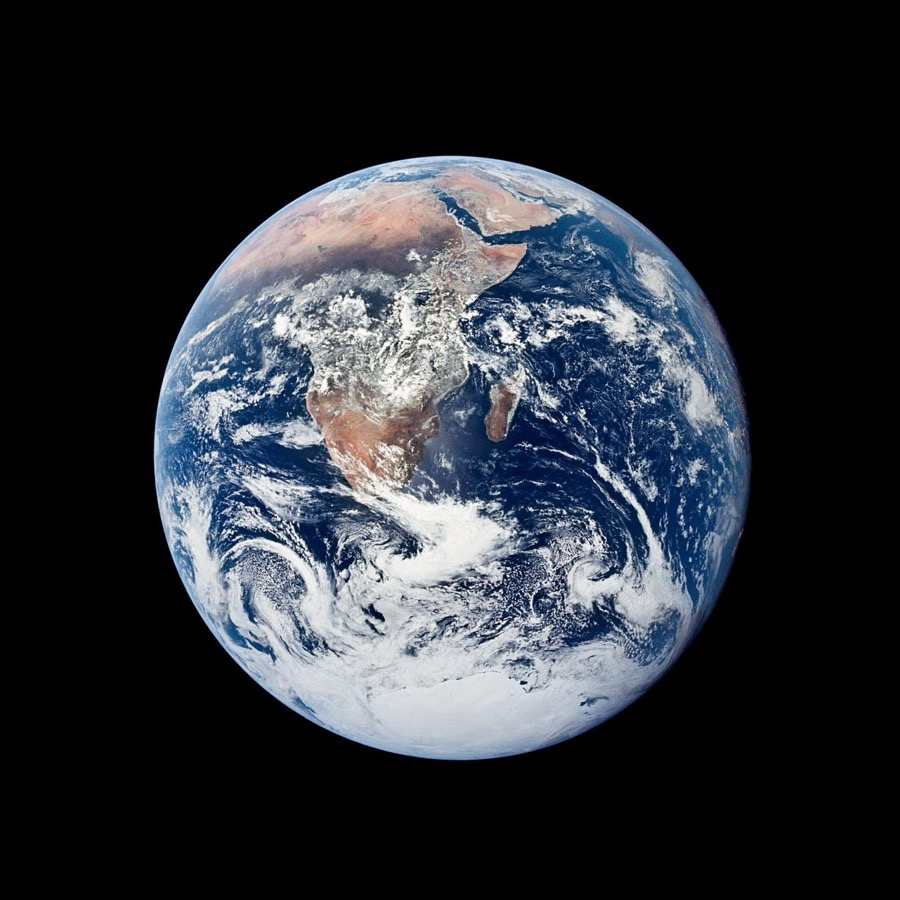
\includegraphics[width=0.55\linewidth]{images/blue-marble-nasa.jpg}
  \caption{Beispielabbildung mit Quellenangabe~\cite{nasa-blue-marble}}
  \label{abb:blue-marble}
\end{figure}

Vektorgrafiken haben gegenüber Screenshots den Vorteil, dass

\begin{itemize}
  \item sie jederzeit editiert werden können,
  \item sie beliebig skaliert werden können, ohne unscharf zu werden,
  \item alle Grafiken einheitlich vergrößert oder verkleinert werden können.
        Das verbessert das Layout ungemein.
\end{itemize}

Abbildungen stehen immer alleinstehend und zentriert. Die Breite wird
relativ zur Textbreite angegeben (\lstinline|width=0.75\linewidth|), damit
sie nie über den Satzspiegel hinausragt. Sollen mehrere Grafiken
nebeneinander stehen, verwendet dafür zwei \lstinline|minipage|-Umgebungen
innerhalb einer \lstinline|figure|.

Die Positionierung übernimmt \LaTeX. Die Angabe \lstinline|[htbp]| erlaubt
es, die Abbildung an die Stelle im Text, an den Seitenanfang, an das
Seitenende oder auf eine eigene Seite zu setzen. Eine Abbildung kann dadurch
auf der Folgeseite landen -- das ist beabsichtigt und kein Fehler.

\subsection{Beschriftungen}

Alle Grafiken und Tabellen sind zu beschriften und mit Quellenangaben zu
versehen. Im Text muss auf jede Abbildung und jede Tabelle Bezug genommen
werden.

Die Beschriftung erfolgt mit \lstinline|\caption| innerhalb der
\lstinline|figure|- bzw.\ \lstinline|table|-Umgebung. Nur so werden
Abbildungs- und Tabellenverzeichnis korrekt geführt. Bei Abbildungen steht
die Beschriftung unter der Grafik, bei Tabellen darüber; die Vorlage stellt
das automatisch richtig ein.

Abbildungen werden mit \enquote{Abb.} und Tabellen mit \enquote{Tab.}
bezeichnet. Auch das erledigt die Vorlage; die Nummerierung läuft
durchgehend und nicht kapitelweise. In englischsprachigen Diplomarbeiten
wird \enquote{Abb.} durch \enquote{Fig.} ersetzt -- dafür genügt die
Klassenoption \lstinline|englisch|.

Unmittelbar nach \lstinline|\caption| gehört ein \lstinline|\label|. Ohne
Label lässt sich die Abbildung später nicht referenzieren. Bewährt hat sich
ein Präfix je Objektart: \lstinline|abb:|, \lstinline|tab:| und
\lstinline|code:|.

\subsection{Querverweise}

Textpassagen, die sich auf andere Kapitel, Grafiken oder Tabellen beziehen,
müssen eine Referenz enthalten. Diese wird mit \lstinline|\ref| erzeugt und
enthält zumindest die Kategorie und die Nummer, also etwa
\lstinline|Abb.~\ref{abb:aufbau}|. Das geschützte Leerzeichen
\lstinline|~| verhindert, dass zwischen Bezeichnung und Nummer umgebrochen
wird.

Liegen referenzierender Text und referenziertes Objekt mehr als eine Seite
auseinander, ist zusätzlich die Seitenzahl mit \lstinline|\pageref|
anzugeben.

Anders als in Word müssen Querverweise und Verzeichnisse nicht manuell
aktualisiert werden. \LaTeX{} löst sie beim Übersetzen auf, benötigt dafür
aber mehrere Durchläufe. \lstinline|latexmk| (bzw.\ \lstinline|make pdf|)
wiederholt den Lauf so lange, bis sich nichts mehr ändert. Meldet das
Protokoll am Ende \enquote{There were undefined references}, fehlt ein
\lstinline|\label| oder es ist falsch geschrieben.

\subsection{Quellenangaben}

In wissenschaftlichen Arbeiten ist es verpflichtend, die Quelle jeder
Aussage anzugeben, die nicht von einem selbst stammt. Der Leser muss die
Möglichkeit haben, die Ausführungen des Autors nachzuprüfen.

Zu diesem Zweck müssen im Text der Diplomarbeit alle verwendeten Quellen
(Fachbücher, Fachzeitschriften, Herstellerunterlagen, Webseiten, \ldots)
angegeben werden. Dies geschieht am Ende des zitierten Textes durch Angabe
der Quelle. Informationen aus Lehrbüchern können als Allgemeinwissen
vorausgesetzt werden und müssen nicht zitiert werden.

Bei inhaltlichen Zitaten, dem Normalfall in technischen Arbeiten, wird der
Inhalt der Quelle nur sinngemäß wiedergegeben.

Bei wörtlichen Zitaten, die in technischen Arbeiten eher selten auftreten,
wird die wörtlich zitierte Textstelle zwischen Anführungszeichen gesetzt,
dahinter steht die Quellenangabe. Eigene Kommentare im Zitat oder
Verkürzungen werden in eckigen Klammern angegeben. Kurze Zitate stehen mit
\lstinline|\zitat| im Fließtext, längere in der Umgebung
\lstinline|zitatfreistehend|.

Beispiel für ein Zitat im Text der Diplomarbeit:
\zitat{[\ldots] kann in diesem Fall eine relationale Datenbank vorteilhaft
eingesetzt werden}~\cite{beispiel-buch}.

Beispiel für ein Zitat als eigener Absatz:

\begin{zitatfreistehend}
  \enquote{The basic guideline for citing online sources is to follow the
  standard citation for the citation, or add the DOI in place of page
  numbers if the source is not paginated.}~\cite{beispiel-artikel}
\end{zitatfreistehend}

Für Diplomarbeiten an der \ac{HTL} Donaustadt ist der IEEE-Zitierstil zu
verwenden. Jeder Quelle wird eine Nummer zugeordnet und in eckigen Klammern
angegeben. Diese Vorlage stellt den Stil bereits ein; zitiert wird mit
\lstinline|\cite{schluessel}|, wobei der Schlüssel aus
\lstinline|references.bib| stammt. Das Quellenverzeichnis wird daraus
automatisch erzeugt und enthält nur tatsächlich zitierte Einträge.

Zum Verwalten der Quellen empfiehlt sich Zotero mit dem Plug-in Better
BibTeX, das \lstinline|references.bib| bei jeder Änderung automatisch neu
exportiert.

Es gibt viele verschiedene Typen von Quellen. Tab.~\ref{tab:quellentypen}
zeigt die häufigsten, den passenden BibTeX-Eintragstyp und die
Informationen, die mindestens enthalten sein sollten.

\begin{table}[htbp]
  \centering
  \caption{Quellentypen}
  \label{tab:quellentypen}
  \begin{tabular}{@{}p{0.28\linewidth}p{0.16\linewidth}p{0.46\linewidth}@{}}
    \toprule
    \tabkopf{Quellentyp} & \tabkopf{Eintragstyp} &
      \tabkopf{wichtigste Informationen} \\
    \midrule
    Buch (auch E-Books, Broschüren) & \lstinline|@book| &
      Autor(en), Titel, Auflage, Verlag, Ort, ISBN \\
    Diplomarbeit, Dissertation & \lstinline|@thesis| &
      Autor(en), Titel, Institution, Ort, Datum \\
    Webseite (auch PDF) & \lstinline|@online| &
      Autor(en), Titel, URL, Abrufdatum (\lstinline|urldate|) \\
    Zeitschriftenartikel & \lstinline|@article| &
      Autor(en), Titel, Publikation, Band, Ausgabe, Seiten, Datum \\
    Verwendung von KI & \lstinline|@online| &
      siehe Anhang und die Vorgaben des Ministeriums~\cite{beispiel-online} \\
    \bottomrule
  \end{tabular}
\end{table}

\subsection{Befehle und Umgebungen}

In Word übernehmen Formatvorlagen das einheitliche Layout. In \LaTeX{}
erfüllen Befehle und Umgebungen dieselbe Aufgabe: Der Text beschreibt, was
etwas \emph{ist}, das Aussehen legt die Dokumentklasse \lstinline|htldon.cls|
zentral fest. Dadurch lässt sich die Formatierung nachträglich an einer
einzigen Stelle ändern.

Die in Tab.~\ref{tab:befehle} aufgeführten Befehle stellen sicher, dass alle
Diplomarbeiten den Richtlinien entsprechen. Sie dürfen nur in begründeten
Ausnahmefällen angepasst werden.

\begin{table}[htbp]
  \centering
  \caption{Befehle und Umgebungen der Vorlage}
  \label{tab:befehle}
  \begin{tabular}{@{}p{0.36\linewidth}p{0.58\linewidth}@{}}
    \toprule
    \tabkopf{Befehl} & \tabkopf{Beschreibung} \\
    \midrule
    \lstinline|\chapter| bis \lstinline|\subsubsection| &
      Kapitelüberschriften mit Dezimalklassifikation. Die ersten drei Ebenen
      erscheinen im Inhaltsverzeichnis, \lstinline|\subsubsection| nicht. \\
    \lstinline|\paragraph| &
      Zwischenüberschrift ohne Nummerierung, nicht im Inhaltsverzeichnis. \\
    \lstinline|\abschnittsautor| &
      Verfasser/in eines Abschnitts, erscheint rechts in der Kopfzeile.
      Format: erster Buchstabe des Vornamens, Punkt, Nachname
      (\enquote{M. Muster}). \\
    \lstinline|\zitat|, \lstinline|zitatfreistehend| &
      Kennzeichnung wörtlicher Zitate im Fließtext bzw.\ als eigener Absatz. \\
    \lstinline|\menue| &
      Menüstrukturen (\menue{Datei / Öffnen}) und Tastatureingaben
      (\menue{Strg + A}). \\
    \lstinline|lstlisting|, \lstinline|\lstinline| &
      Quellcode als eigener Block bzw.\ im Fließtext. \\
    \lstinline|\tabkopf| &
      Kopfzeile einer Tabelle. Der Tabelleninhalt selbst wird von der Klasse
      automatisch auf 10\,pt und linksbündig gestellt. \\
    \lstinline|\ac|, \lstinline|\acp| &
      Abkürzung, beim ersten Auftreten ausgeschrieben, im Plural mit
      \lstinline|\acp|. \\
    \lstinline|\cite|, \lstinline|\ref|, \lstinline|\pageref| &
      Quellenangabe, Querverweis, Seitenverweis. \\
    \bottomrule
  \end{tabular}
\end{table}

Überschriften der Kapitel müssen kurz, präzise und selbsterklärend sein.
Beispiele für unzureichende Überschriften: \enquote{5.3 Aufbau},
\enquote{5.3 Messergebnis}, \enquote{5.3 Beispiel}.

Bei Unterüberschriften gilt:

\begin{itemize}
  \item Es muss mindestens zwei Unterpunkte geben. Ein Abschnitt 3.2.1 darf
        daher nicht existieren, wenn kein 3.2.2 folgt.
  \item Unterpunkte sollten inhaltlich ausreichend gefüllt sein und
        mindestens eine halbe Seite umfassen.
  \item Unterpunkte, die lediglich aus einem einzelnen Satz bestehen, werden
        besser als Aufzählung dargestellt.
\end{itemize}

Für die Darstellung von Quellcode gilt:

\begin{itemize}
  \item Umfang:
        \begin{itemize}
          \item Der vollständige Sourcecode gehört ausschließlich auf das
                elektronische Speichermedium.
          \item Im Dokument selbst sollen nur wesentliche Ausschnitte
                aufgenommen werden.
        \end{itemize}
  \item Formatierung: Schriftart und Schriftgröße gibt die
        \lstinline|lstlisting|-Umgebung vor, der Zeilenabstand ist dort
        einzeilig. Die Sprache wird mit
        \lstinline|[language=Python]| angegeben, damit die
        Syntaxhervorhebung stimmt.
  \item Inhaltliche Anforderungen: Der Sourcecode muss ausreichend
        kommentiert sein.
  \item Verwendung im Fließtext: Wird Sourcecode im Text erwähnt, ist
        \lstinline|\lstinline| zu verwenden. Zusätzliche Anführungszeichen
        sind nicht erforderlich. Beispiel: Mit dem Befehl
        \lstinline|ShowModal| wird ein Frame geöffnet.
\end{itemize}

\section{Beschreibung der Kapitel}

\subsection{Titelseite}

Die Titelseite wird vollständig aus \lstinline|metadata.tex| erzeugt. Dort
sind einzutragen:

\begin{itemize}
  \item der Titel der Diplomarbeit mit \lstinline|\titel|. Er wird
        automatisch in die Kopfzeile übernommen.
  \item ein Projektlogo, Bild oder eine Zeichnung mit
        \lstinline|\projektlogo|.
  \item alle Verfasser/innen mit \lstinline|\teammitglied| und die
        Betreuung mit \lstinline|\betreuung|.
  \item Schuljahr, Abteilung und Klasse.
\end{itemize}

Falls alle Verfasser/innen oder Betreuer/innen dasselbe Geschlecht haben,
kann die geschlechtsspezifische Form verwendet werden; dafür ist das
optionale Argument von \lstinline|\betreuung| vorgesehen.

\subsection{Verfassererklärung}

In der Verfassererklärung bekennen sich die Verfasser/innen zu einem
wissenschaftlichen Arbeitsstil. Sollten im Nachhinein grobe Verstöße dagegen
aufgedeckt werden, kann die Arbeit für ungültig erklärt und der Abschluss
revidiert werden.

Die Erklärung erzeugt \lstinline|\eigenstaendigkeitserklaerung|. Je
Teammitglied entsteht automatisch eine Unterschriftszeile. Zu ergänzen sind
gegebenenfalls Kooperationen mit Firmen und Sperrvermerke.

\subsection{Problemstellung}

Die Seite \enquote{Problemstellung} wird durch den eingescannten Antrag (mit
allen Stempeln und Unterschriften) vollflächig ersetzt. Dazu wird in
\lstinline|frontmatter/problem-statement.tex| das Scan-PDF eingebunden.

\subsection{Kurzfassung bzw.\ Abstract}

Die Kurzfassung bzw.\ der Abstract soll kurz, prägnant und verständlich den
Inhalt der Arbeit wiedergeben: Zielsetzung, Ablauf, wichtigste Erkenntnisse,
wesentliche Merkmale des realisierten Produkts, Schlussfolgerungen und
Ausblick. Beide sind als eigenständiges Dokument zu konzipieren, das
unabhängig von der Diplomarbeit gelesen und verstanden werden kann, und
sollen in Deutsch und Englisch jeweils nicht mehr als eine Seite umfassen.

\subsection{Inhaltsverzeichnis}

Das Inhaltsverzeichnis wird automatisch aus den Überschriften erstellt. Es
zeigt die ersten drei Ebenen, der Text steht linksbündig, die Seitenzahlen
rechtsbündig, als Füllzeichen dienen Punkte. Eine manuelle Aktualisierung
ist nicht nötig.

\subsection{Die weiteren Kapitel}

Die Kapitel Projektplanung, Technische Grundlagen, Praktische Realisierung
sowie Evaluierung und Ergebnisse beschreiben die Diplomarbeit im Detail.

Für die Beurteilung ist es wichtig, den/die Verfasser/in zu kennen. Daher
ist dieser Hinweis auf jeder Seite rechtsbündig in der Kopfzeile zu
vermerken. Dafür wird \lstinline|\abschnittsautor| direkt nach der
Überschrift gesetzt; der Eintrag gilt ab dort bis zur nächsten Angabe.
Haben mehrere Personen gemeinsam an einem Abschnitt gearbeitet, sind alle zu
nennen, durch Komma getrennt:
\lstinline|\abschnittsautor{A. Erste, B. Zweite}|.

Die Projektplanung soll die systematische Durchführung der Diplomarbeit
innerhalb des Projektteams beschreiben. Dabei sollen geplante Ziele und
tatsächlich erreichte Ergebnisse miteinander verglichen und die Unterschiede
reflektiert werden. Beim klassischen Wasserfall-Projektmanagement können
etwa die Meilensteine als Referenz dienen, bei agiler Projektorganisation
die Sprint-Reviews.

Im Kapitel Technische Grundlagen finden sich alle für das unmittelbare
technische Verständnis der Diplomarbeit relevanten Inhalte. Hier wird
insbesondere auf korrekte Zitate und den sorgfältigen Einsatz von Quellen
geachtet.

Das Kapitel Praktische Realisierung enthält die praktischen Eigenleistungen
der Diplomarbeit. Dabei sollen die Vorgänge und Untersuchungen beschrieben
und nachvollziehbar dokumentiert werden.

Im Kapitel Evaluierung und Ergebnisse erfolgt die Darstellung und Bewertung
der abschließenden Arbeit. Hier soll ebenso, sofern vorhanden, das
Endprodukt bzw.\ der Prototyp präsentiert und beschrieben werden.

\subsection{Anhang}

Im Anhang können alle Informationen gesammelt werden, die zwar zur
Diplomarbeit gehören, jedoch im Inhaltsteil den Rahmen gesprengt hätten.
Dazu zählen wichtige Notizen (z.\,B. Gesprächsprotokolle), Normen,
Schnittstellendefinitionen oder Präsentationen. Weiters soll der Anhang den
Inhalt eines beigefügten elektronischen Speichermediums sowie einen
einseitigen Lebenslauf jedes Teammitglieds enthalten.

Verpflichtend ist außerdem die Dokumentation aller eingesetzten KI-basierten
Hilfsmittel. Dafür ist \lstinline|appendix/ai-tools.tex| vorgesehen.

% in diplomarbeit.tex entfernen und diese Datei mitlöschen.
% =====================================================================
\chapter{Richtlinie für das Verfassen von Diplomarbeiten}

Diese Richtlinie beschreibt die formalen und inhaltlichen Anforderungen an
eine wissenschaftliche Publikation und soll ein einheitliches
Erscheinungsbild der Diplomarbeiten sicherstellen. Dieses Kapitel beschreibt
weiters, wie die vorliegende Diplomarbeitsvorlage zu verwenden ist, und ist
im finalen Dokument zu entfernen.

Es sind bewusst nur die wesentlichen Punkte festgelegt. In Absprache mit dem
Betreuer/der Betreuerin soll stets Freiraum für die individuelle Gestaltung
sowie projektbedingte Erfordernisse bleiben.

\section{Allgemein}

Die Diplomarbeit soll kurz und prägnant -- aber vollständig -- gehalten sein
und einen Umfang von ca.\ 70 Seiten (ohne Anhang) bei einer Teamgröße von
2 Personen umfassen. Die inhaltliche Qualität bei in Umfang eingeschränkter
Darstellung ist ein wesentliches Ziel jeder wissenschaftlichen Publikation
und wird auch in die Beurteilung einbezogen. Grafische Darstellungen,
Übersichtstabellen und Diagramme sind wichtige Hilfsmittel, um diese Vorgabe
einhalten zu können.

Einige Tipps:

\begin{itemize}
  \item Das Verwenden der \enquote{ich}- und \enquote{wir}-Form sowie von
        \enquote{man}-Aussagen ist zu vermeiden.
  \item Abkürzungen müssen unmittelbar nach ihrem ersten Auftreten erläutert
        werden; falls erforderlich, ist ein Abkürzungsverzeichnis zu
        erstellen. Der Befehl \lstinline|\ac{API}| erledigt das automatisch:
        beim ersten Auftreten schreibt er die Abkürzung aus, danach nicht
        mehr.
  \item Über Themen, die nur indirekt mit der gestellten Aufgabe zu tun
        haben, soll nicht berichtet werden. Die ausführliche Darstellung von
        Grundlagenwissen ist nicht erforderlich; meistens reicht das Zitieren
        geeigneter Quellen.
  \item Arbeitet im Team über ein Git-Repository und legt pro Kapitel eine
        eigene Datei an. So lassen sich Änderungen nachvollziehen und
        Konflikte auf einzelne Absätze eingrenzen.
\end{itemize}

\subsection{Platzhalter in dieser Vorlage}

Alle Beispieltexte in dieser Vorlage sind zu ersetzen oder zu löschen. Das
betrifft insbesondere:

\begin{itemize}
  \item die Metadaten in \lstinline|metadata.tex| (Titel, Team, Betreuung,
        Schuljahr, Klasse),
  \item die Beispielkapitel in \lstinline|chapters/|,
  \item die Beispielquellen in \lstinline|references.bib|,
  \item das Abkürzungsverzeichnis in \lstinline|diplomarbeit.tex|,
  \item dieses gesamte Kapitel~6.
\end{itemize}

Um dieses Kapitel zu entfernen, genügt es, in \lstinline|diplomarbeit.tex|
die Zeile \lstinline|% =====================================================================
% Kapitel 6 der Abteilungsvorlage, auf LaTeX übertragen.
% Vor der Abgabe komplett löschen: die Zeile % =====================================================================
% Kapitel 6 der Abteilungsvorlage, auf LaTeX übertragen.
% Vor der Abgabe komplett löschen: die Zeile \input{chapters/06-guideline}
% in diplomarbeit.tex entfernen und diese Datei mitlöschen.
% =====================================================================
\chapter{Richtlinie für das Verfassen von Diplomarbeiten}

Diese Richtlinie beschreibt die formalen und inhaltlichen Anforderungen an
eine wissenschaftliche Publikation und soll ein einheitliches
Erscheinungsbild der Diplomarbeiten sicherstellen. Dieses Kapitel beschreibt
weiters, wie die vorliegende Diplomarbeitsvorlage zu verwenden ist, und ist
im finalen Dokument zu entfernen.

Es sind bewusst nur die wesentlichen Punkte festgelegt. In Absprache mit dem
Betreuer/der Betreuerin soll stets Freiraum für die individuelle Gestaltung
sowie projektbedingte Erfordernisse bleiben.

\section{Allgemein}

Die Diplomarbeit soll kurz und prägnant -- aber vollständig -- gehalten sein
und einen Umfang von ca.\ 70 Seiten (ohne Anhang) bei einer Teamgröße von
2 Personen umfassen. Die inhaltliche Qualität bei in Umfang eingeschränkter
Darstellung ist ein wesentliches Ziel jeder wissenschaftlichen Publikation
und wird auch in die Beurteilung einbezogen. Grafische Darstellungen,
Übersichtstabellen und Diagramme sind wichtige Hilfsmittel, um diese Vorgabe
einhalten zu können.

Einige Tipps:

\begin{itemize}
  \item Das Verwenden der \enquote{ich}- und \enquote{wir}-Form sowie von
        \enquote{man}-Aussagen ist zu vermeiden.
  \item Abkürzungen müssen unmittelbar nach ihrem ersten Auftreten erläutert
        werden; falls erforderlich, ist ein Abkürzungsverzeichnis zu
        erstellen. Der Befehl \lstinline|\ac{API}| erledigt das automatisch:
        beim ersten Auftreten schreibt er die Abkürzung aus, danach nicht
        mehr.
  \item Über Themen, die nur indirekt mit der gestellten Aufgabe zu tun
        haben, soll nicht berichtet werden. Die ausführliche Darstellung von
        Grundlagenwissen ist nicht erforderlich; meistens reicht das Zitieren
        geeigneter Quellen.
  \item Arbeitet im Team über ein Git-Repository und legt pro Kapitel eine
        eigene Datei an. So lassen sich Änderungen nachvollziehen und
        Konflikte auf einzelne Absätze eingrenzen.
\end{itemize}

\subsection{Platzhalter in dieser Vorlage}

Alle Beispieltexte in dieser Vorlage sind zu ersetzen oder zu löschen. Das
betrifft insbesondere:

\begin{itemize}
  \item die Metadaten in \lstinline|metadata.tex| (Titel, Team, Betreuung,
        Schuljahr, Klasse),
  \item die Beispielkapitel in \lstinline|chapters/|,
  \item die Beispielquellen in \lstinline|references.bib|,
  \item das Abkürzungsverzeichnis in \lstinline|diplomarbeit.tex|,
  \item dieses gesamte Kapitel~6.
\end{itemize}

Um dieses Kapitel zu entfernen, genügt es, in \lstinline|diplomarbeit.tex|
die Zeile \lstinline|\input{chapters/06-guideline}| zu löschen. Die Einträge
im Inhaltsverzeichnis und in den übrigen Verzeichnissen verschwinden beim
nächsten Übersetzen von selbst.

\subsection{Abgabe der Diplomarbeit}

Die Diplomarbeit ist in gedruckter bzw.\ gebundener Form und in digitaler
Form vorzulegen. Dem Abteilungsvorstand sind zwei geheftete Exemplare (ein
Belegexemplar und ein Beurteilungsexemplar für den/die Betreuer/in) zu
übergeben.

Nach erfolgter Beurteilung geht das Beurteilungsexemplar temporär zurück an
die Diplomarbeitsgruppe. Nun können letzte Korrekturen (ohne
Beurteilungsrelevanz) vorgenommen werden. Anschließend wird die Arbeit erneut
ausgedruckt und gesammelt zur Bindung außer Haus gegeben. Weitere Exemplare
für Kooperationspartner (Firmen, Institutionen) oder Projektteilnehmer können
in diesem Zusammenhang erstellt werden.

\subsection{Grafiken}

Abbildungen müssen in gut lesbarer Bildqualität eingefügt werden. Grafiken
sollten am besten in einem vektorbasierten Zeichenprogramm (z.\,B. Inkscape,
draw.io) erstellt und als PDF exportiert werden; PDF und PNG lassen sich
direkt einbinden, SVG nicht. Alle Bilddateien gehören in den Ordner
\lstinline|images/|.

\begin{lstlisting}[language={[LaTeX]TeX}, caption={Eine Abbildung einbinden},
                   label=code:abbildung]
\begin{figure}[htbp]
  \centering
  
\includegraphics[width=0.75\linewidth]{images/example-figure.pdf}
  \caption{Aufbau des Systems}
  \label{abb:aufbau}
\end{figure}
\end{lstlisting}

Abb.~\ref{abb:blue-marble} zeigt, wie das Ergebnis aussieht. Stammt die
Grafik nicht von euch selbst, gehört die Quelle in die Beschriftung.

\begin{figure}[htbp]
  \centering
  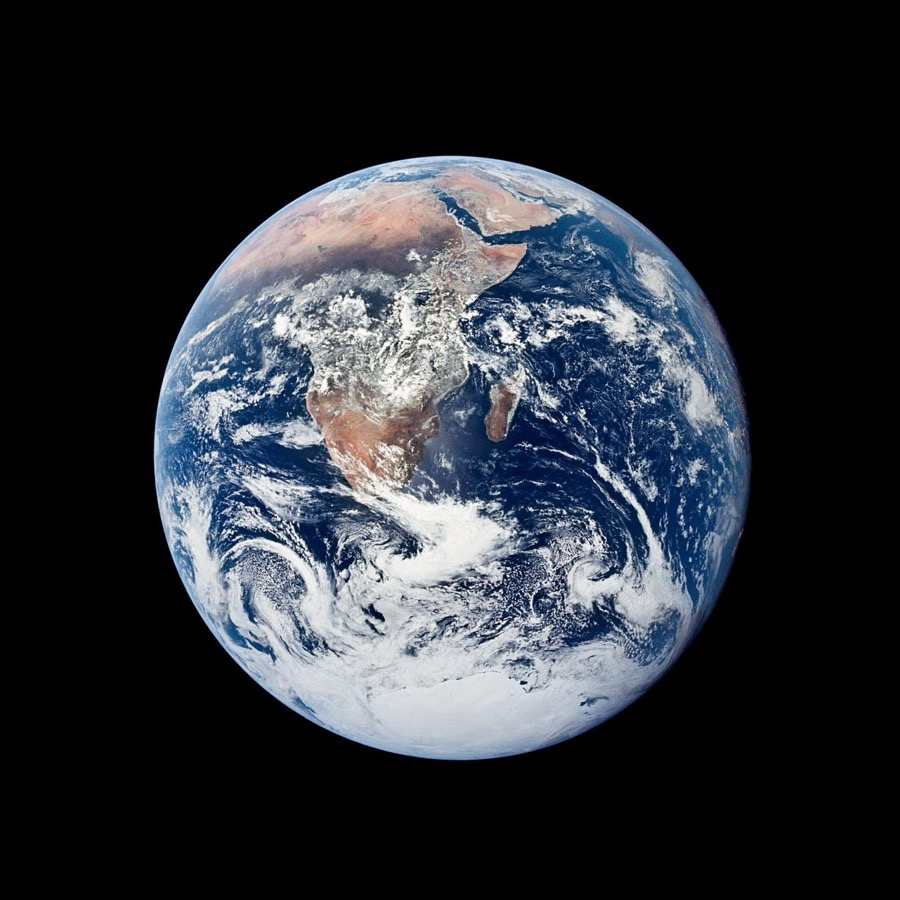
\includegraphics[width=0.55\linewidth]{images/blue-marble-nasa.jpg}
  \caption{Beispielabbildung mit Quellenangabe~\cite{nasa-blue-marble}}
  \label{abb:blue-marble}
\end{figure}

Vektorgrafiken haben gegenüber Screenshots den Vorteil, dass

\begin{itemize}
  \item sie jederzeit editiert werden können,
  \item sie beliebig skaliert werden können, ohne unscharf zu werden,
  \item alle Grafiken einheitlich vergrößert oder verkleinert werden können.
        Das verbessert das Layout ungemein.
\end{itemize}

Abbildungen stehen immer alleinstehend und zentriert. Die Breite wird
relativ zur Textbreite angegeben (\lstinline|width=0.75\linewidth|), damit
sie nie über den Satzspiegel hinausragt. Sollen mehrere Grafiken
nebeneinander stehen, verwendet dafür zwei \lstinline|minipage|-Umgebungen
innerhalb einer \lstinline|figure|.

Die Positionierung übernimmt \LaTeX. Die Angabe \lstinline|[htbp]| erlaubt
es, die Abbildung an die Stelle im Text, an den Seitenanfang, an das
Seitenende oder auf eine eigene Seite zu setzen. Eine Abbildung kann dadurch
auf der Folgeseite landen -- das ist beabsichtigt und kein Fehler.

\subsection{Beschriftungen}

Alle Grafiken und Tabellen sind zu beschriften und mit Quellenangaben zu
versehen. Im Text muss auf jede Abbildung und jede Tabelle Bezug genommen
werden.

Die Beschriftung erfolgt mit \lstinline|\caption| innerhalb der
\lstinline|figure|- bzw.\ \lstinline|table|-Umgebung. Nur so werden
Abbildungs- und Tabellenverzeichnis korrekt geführt. Bei Abbildungen steht
die Beschriftung unter der Grafik, bei Tabellen darüber; die Vorlage stellt
das automatisch richtig ein.

Abbildungen werden mit \enquote{Abb.} und Tabellen mit \enquote{Tab.}
bezeichnet. Auch das erledigt die Vorlage; die Nummerierung läuft
durchgehend und nicht kapitelweise. In englischsprachigen Diplomarbeiten
wird \enquote{Abb.} durch \enquote{Fig.} ersetzt -- dafür genügt die
Klassenoption \lstinline|englisch|.

Unmittelbar nach \lstinline|\caption| gehört ein \lstinline|\label|. Ohne
Label lässt sich die Abbildung später nicht referenzieren. Bewährt hat sich
ein Präfix je Objektart: \lstinline|abb:|, \lstinline|tab:| und
\lstinline|code:|.

\subsection{Querverweise}

Textpassagen, die sich auf andere Kapitel, Grafiken oder Tabellen beziehen,
müssen eine Referenz enthalten. Diese wird mit \lstinline|\ref| erzeugt und
enthält zumindest die Kategorie und die Nummer, also etwa
\lstinline|Abb.~\ref{abb:aufbau}|. Das geschützte Leerzeichen
\lstinline|~| verhindert, dass zwischen Bezeichnung und Nummer umgebrochen
wird.

Liegen referenzierender Text und referenziertes Objekt mehr als eine Seite
auseinander, ist zusätzlich die Seitenzahl mit \lstinline|\pageref|
anzugeben.

Anders als in Word müssen Querverweise und Verzeichnisse nicht manuell
aktualisiert werden. \LaTeX{} löst sie beim Übersetzen auf, benötigt dafür
aber mehrere Durchläufe. \lstinline|latexmk| (bzw.\ \lstinline|make pdf|)
wiederholt den Lauf so lange, bis sich nichts mehr ändert. Meldet das
Protokoll am Ende \enquote{There were undefined references}, fehlt ein
\lstinline|\label| oder es ist falsch geschrieben.

\subsection{Quellenangaben}

In wissenschaftlichen Arbeiten ist es verpflichtend, die Quelle jeder
Aussage anzugeben, die nicht von einem selbst stammt. Der Leser muss die
Möglichkeit haben, die Ausführungen des Autors nachzuprüfen.

Zu diesem Zweck müssen im Text der Diplomarbeit alle verwendeten Quellen
(Fachbücher, Fachzeitschriften, Herstellerunterlagen, Webseiten, \ldots)
angegeben werden. Dies geschieht am Ende des zitierten Textes durch Angabe
der Quelle. Informationen aus Lehrbüchern können als Allgemeinwissen
vorausgesetzt werden und müssen nicht zitiert werden.

Bei inhaltlichen Zitaten, dem Normalfall in technischen Arbeiten, wird der
Inhalt der Quelle nur sinngemäß wiedergegeben.

Bei wörtlichen Zitaten, die in technischen Arbeiten eher selten auftreten,
wird die wörtlich zitierte Textstelle zwischen Anführungszeichen gesetzt,
dahinter steht die Quellenangabe. Eigene Kommentare im Zitat oder
Verkürzungen werden in eckigen Klammern angegeben. Kurze Zitate stehen mit
\lstinline|\zitat| im Fließtext, längere in der Umgebung
\lstinline|zitatfreistehend|.

Beispiel für ein Zitat im Text der Diplomarbeit:
\zitat{[\ldots] kann in diesem Fall eine relationale Datenbank vorteilhaft
eingesetzt werden}~\cite{beispiel-buch}.

Beispiel für ein Zitat als eigener Absatz:

\begin{zitatfreistehend}
  \enquote{The basic guideline for citing online sources is to follow the
  standard citation for the citation, or add the DOI in place of page
  numbers if the source is not paginated.}~\cite{beispiel-artikel}
\end{zitatfreistehend}

Für Diplomarbeiten an der \ac{HTL} Donaustadt ist der IEEE-Zitierstil zu
verwenden. Jeder Quelle wird eine Nummer zugeordnet und in eckigen Klammern
angegeben. Diese Vorlage stellt den Stil bereits ein; zitiert wird mit
\lstinline|\cite{schluessel}|, wobei der Schlüssel aus
\lstinline|references.bib| stammt. Das Quellenverzeichnis wird daraus
automatisch erzeugt und enthält nur tatsächlich zitierte Einträge.

Zum Verwalten der Quellen empfiehlt sich Zotero mit dem Plug-in Better
BibTeX, das \lstinline|references.bib| bei jeder Änderung automatisch neu
exportiert.

Es gibt viele verschiedene Typen von Quellen. Tab.~\ref{tab:quellentypen}
zeigt die häufigsten, den passenden BibTeX-Eintragstyp und die
Informationen, die mindestens enthalten sein sollten.

\begin{table}[htbp]
  \centering
  \caption{Quellentypen}
  \label{tab:quellentypen}
  \begin{tabular}{@{}p{0.28\linewidth}p{0.16\linewidth}p{0.46\linewidth}@{}}
    \toprule
    \tabkopf{Quellentyp} & \tabkopf{Eintragstyp} &
      \tabkopf{wichtigste Informationen} \\
    \midrule
    Buch (auch E-Books, Broschüren) & \lstinline|@book| &
      Autor(en), Titel, Auflage, Verlag, Ort, ISBN \\
    Diplomarbeit, Dissertation & \lstinline|@thesis| &
      Autor(en), Titel, Institution, Ort, Datum \\
    Webseite (auch PDF) & \lstinline|@online| &
      Autor(en), Titel, URL, Abrufdatum (\lstinline|urldate|) \\
    Zeitschriftenartikel & \lstinline|@article| &
      Autor(en), Titel, Publikation, Band, Ausgabe, Seiten, Datum \\
    Verwendung von KI & \lstinline|@online| &
      siehe Anhang und die Vorgaben des Ministeriums~\cite{beispiel-online} \\
    \bottomrule
  \end{tabular}
\end{table}

\subsection{Befehle und Umgebungen}

In Word übernehmen Formatvorlagen das einheitliche Layout. In \LaTeX{}
erfüllen Befehle und Umgebungen dieselbe Aufgabe: Der Text beschreibt, was
etwas \emph{ist}, das Aussehen legt die Dokumentklasse \lstinline|htldon.cls|
zentral fest. Dadurch lässt sich die Formatierung nachträglich an einer
einzigen Stelle ändern.

Die in Tab.~\ref{tab:befehle} aufgeführten Befehle stellen sicher, dass alle
Diplomarbeiten den Richtlinien entsprechen. Sie dürfen nur in begründeten
Ausnahmefällen angepasst werden.

\begin{table}[htbp]
  \centering
  \caption{Befehle und Umgebungen der Vorlage}
  \label{tab:befehle}
  \begin{tabular}{@{}p{0.36\linewidth}p{0.58\linewidth}@{}}
    \toprule
    \tabkopf{Befehl} & \tabkopf{Beschreibung} \\
    \midrule
    \lstinline|\chapter| bis \lstinline|\subsubsection| &
      Kapitelüberschriften mit Dezimalklassifikation. Die ersten drei Ebenen
      erscheinen im Inhaltsverzeichnis, \lstinline|\subsubsection| nicht. \\
    \lstinline|\paragraph| &
      Zwischenüberschrift ohne Nummerierung, nicht im Inhaltsverzeichnis. \\
    \lstinline|\abschnittsautor| &
      Verfasser/in eines Abschnitts, erscheint rechts in der Kopfzeile.
      Format: erster Buchstabe des Vornamens, Punkt, Nachname
      (\enquote{M. Muster}). \\
    \lstinline|\zitat|, \lstinline|zitatfreistehend| &
      Kennzeichnung wörtlicher Zitate im Fließtext bzw.\ als eigener Absatz. \\
    \lstinline|\menue| &
      Menüstrukturen (\menue{Datei / Öffnen}) und Tastatureingaben
      (\menue{Strg + A}). \\
    \lstinline|lstlisting|, \lstinline|\lstinline| &
      Quellcode als eigener Block bzw.\ im Fließtext. \\
    \lstinline|\tabkopf| &
      Kopfzeile einer Tabelle. Der Tabelleninhalt selbst wird von der Klasse
      automatisch auf 10\,pt und linksbündig gestellt. \\
    \lstinline|\ac|, \lstinline|\acp| &
      Abkürzung, beim ersten Auftreten ausgeschrieben, im Plural mit
      \lstinline|\acp|. \\
    \lstinline|\cite|, \lstinline|\ref|, \lstinline|\pageref| &
      Quellenangabe, Querverweis, Seitenverweis. \\
    \bottomrule
  \end{tabular}
\end{table}

Überschriften der Kapitel müssen kurz, präzise und selbsterklärend sein.
Beispiele für unzureichende Überschriften: \enquote{5.3 Aufbau},
\enquote{5.3 Messergebnis}, \enquote{5.3 Beispiel}.

Bei Unterüberschriften gilt:

\begin{itemize}
  \item Es muss mindestens zwei Unterpunkte geben. Ein Abschnitt 3.2.1 darf
        daher nicht existieren, wenn kein 3.2.2 folgt.
  \item Unterpunkte sollten inhaltlich ausreichend gefüllt sein und
        mindestens eine halbe Seite umfassen.
  \item Unterpunkte, die lediglich aus einem einzelnen Satz bestehen, werden
        besser als Aufzählung dargestellt.
\end{itemize}

Für die Darstellung von Quellcode gilt:

\begin{itemize}
  \item Umfang:
        \begin{itemize}
          \item Der vollständige Sourcecode gehört ausschließlich auf das
                elektronische Speichermedium.
          \item Im Dokument selbst sollen nur wesentliche Ausschnitte
                aufgenommen werden.
        \end{itemize}
  \item Formatierung: Schriftart und Schriftgröße gibt die
        \lstinline|lstlisting|-Umgebung vor, der Zeilenabstand ist dort
        einzeilig. Die Sprache wird mit
        \lstinline|[language=Python]| angegeben, damit die
        Syntaxhervorhebung stimmt.
  \item Inhaltliche Anforderungen: Der Sourcecode muss ausreichend
        kommentiert sein.
  \item Verwendung im Fließtext: Wird Sourcecode im Text erwähnt, ist
        \lstinline|\lstinline| zu verwenden. Zusätzliche Anführungszeichen
        sind nicht erforderlich. Beispiel: Mit dem Befehl
        \lstinline|ShowModal| wird ein Frame geöffnet.
\end{itemize}

\section{Beschreibung der Kapitel}

\subsection{Titelseite}

Die Titelseite wird vollständig aus \lstinline|metadata.tex| erzeugt. Dort
sind einzutragen:

\begin{itemize}
  \item der Titel der Diplomarbeit mit \lstinline|\titel|. Er wird
        automatisch in die Kopfzeile übernommen.
  \item ein Projektlogo, Bild oder eine Zeichnung mit
        \lstinline|\projektlogo|.
  \item alle Verfasser/innen mit \lstinline|\teammitglied| und die
        Betreuung mit \lstinline|\betreuung|.
  \item Schuljahr, Abteilung und Klasse.
\end{itemize}

Falls alle Verfasser/innen oder Betreuer/innen dasselbe Geschlecht haben,
kann die geschlechtsspezifische Form verwendet werden; dafür ist das
optionale Argument von \lstinline|\betreuung| vorgesehen.

\subsection{Verfassererklärung}

In der Verfassererklärung bekennen sich die Verfasser/innen zu einem
wissenschaftlichen Arbeitsstil. Sollten im Nachhinein grobe Verstöße dagegen
aufgedeckt werden, kann die Arbeit für ungültig erklärt und der Abschluss
revidiert werden.

Die Erklärung erzeugt \lstinline|\eigenstaendigkeitserklaerung|. Je
Teammitglied entsteht automatisch eine Unterschriftszeile. Zu ergänzen sind
gegebenenfalls Kooperationen mit Firmen und Sperrvermerke.

\subsection{Problemstellung}

Die Seite \enquote{Problemstellung} wird durch den eingescannten Antrag (mit
allen Stempeln und Unterschriften) vollflächig ersetzt. Dazu wird in
\lstinline|frontmatter/problem-statement.tex| das Scan-PDF eingebunden.

\subsection{Kurzfassung bzw.\ Abstract}

Die Kurzfassung bzw.\ der Abstract soll kurz, prägnant und verständlich den
Inhalt der Arbeit wiedergeben: Zielsetzung, Ablauf, wichtigste Erkenntnisse,
wesentliche Merkmale des realisierten Produkts, Schlussfolgerungen und
Ausblick. Beide sind als eigenständiges Dokument zu konzipieren, das
unabhängig von der Diplomarbeit gelesen und verstanden werden kann, und
sollen in Deutsch und Englisch jeweils nicht mehr als eine Seite umfassen.

\subsection{Inhaltsverzeichnis}

Das Inhaltsverzeichnis wird automatisch aus den Überschriften erstellt. Es
zeigt die ersten drei Ebenen, der Text steht linksbündig, die Seitenzahlen
rechtsbündig, als Füllzeichen dienen Punkte. Eine manuelle Aktualisierung
ist nicht nötig.

\subsection{Die weiteren Kapitel}

Die Kapitel Projektplanung, Technische Grundlagen, Praktische Realisierung
sowie Evaluierung und Ergebnisse beschreiben die Diplomarbeit im Detail.

Für die Beurteilung ist es wichtig, den/die Verfasser/in zu kennen. Daher
ist dieser Hinweis auf jeder Seite rechtsbündig in der Kopfzeile zu
vermerken. Dafür wird \lstinline|\abschnittsautor| direkt nach der
Überschrift gesetzt; der Eintrag gilt ab dort bis zur nächsten Angabe.
Haben mehrere Personen gemeinsam an einem Abschnitt gearbeitet, sind alle zu
nennen, durch Komma getrennt:
\lstinline|\abschnittsautor{A. Erste, B. Zweite}|.

Die Projektplanung soll die systematische Durchführung der Diplomarbeit
innerhalb des Projektteams beschreiben. Dabei sollen geplante Ziele und
tatsächlich erreichte Ergebnisse miteinander verglichen und die Unterschiede
reflektiert werden. Beim klassischen Wasserfall-Projektmanagement können
etwa die Meilensteine als Referenz dienen, bei agiler Projektorganisation
die Sprint-Reviews.

Im Kapitel Technische Grundlagen finden sich alle für das unmittelbare
technische Verständnis der Diplomarbeit relevanten Inhalte. Hier wird
insbesondere auf korrekte Zitate und den sorgfältigen Einsatz von Quellen
geachtet.

Das Kapitel Praktische Realisierung enthält die praktischen Eigenleistungen
der Diplomarbeit. Dabei sollen die Vorgänge und Untersuchungen beschrieben
und nachvollziehbar dokumentiert werden.

Im Kapitel Evaluierung und Ergebnisse erfolgt die Darstellung und Bewertung
der abschließenden Arbeit. Hier soll ebenso, sofern vorhanden, das
Endprodukt bzw.\ der Prototyp präsentiert und beschrieben werden.

\subsection{Anhang}

Im Anhang können alle Informationen gesammelt werden, die zwar zur
Diplomarbeit gehören, jedoch im Inhaltsteil den Rahmen gesprengt hätten.
Dazu zählen wichtige Notizen (z.\,B. Gesprächsprotokolle), Normen,
Schnittstellendefinitionen oder Präsentationen. Weiters soll der Anhang den
Inhalt eines beigefügten elektronischen Speichermediums sowie einen
einseitigen Lebenslauf jedes Teammitglieds enthalten.

Verpflichtend ist außerdem die Dokumentation aller eingesetzten KI-basierten
Hilfsmittel. Dafür ist \lstinline|appendix/ai-tools.tex| vorgesehen.

% in diplomarbeit.tex entfernen und diese Datei mitlöschen.
% =====================================================================
\chapter{Richtlinie für das Verfassen von Diplomarbeiten}

Diese Richtlinie beschreibt die formalen und inhaltlichen Anforderungen an
eine wissenschaftliche Publikation und soll ein einheitliches
Erscheinungsbild der Diplomarbeiten sicherstellen. Dieses Kapitel beschreibt
weiters, wie die vorliegende Diplomarbeitsvorlage zu verwenden ist, und ist
im finalen Dokument zu entfernen.

Es sind bewusst nur die wesentlichen Punkte festgelegt. In Absprache mit dem
Betreuer/der Betreuerin soll stets Freiraum für die individuelle Gestaltung
sowie projektbedingte Erfordernisse bleiben.

\section{Allgemein}

Die Diplomarbeit soll kurz und prägnant -- aber vollständig -- gehalten sein
und einen Umfang von ca.\ 70 Seiten (ohne Anhang) bei einer Teamgröße von
2 Personen umfassen. Die inhaltliche Qualität bei in Umfang eingeschränkter
Darstellung ist ein wesentliches Ziel jeder wissenschaftlichen Publikation
und wird auch in die Beurteilung einbezogen. Grafische Darstellungen,
Übersichtstabellen und Diagramme sind wichtige Hilfsmittel, um diese Vorgabe
einhalten zu können.

Einige Tipps:

\begin{itemize}
  \item Das Verwenden der \enquote{ich}- und \enquote{wir}-Form sowie von
        \enquote{man}-Aussagen ist zu vermeiden.
  \item Abkürzungen müssen unmittelbar nach ihrem ersten Auftreten erläutert
        werden; falls erforderlich, ist ein Abkürzungsverzeichnis zu
        erstellen. Der Befehl \lstinline|\ac{API}| erledigt das automatisch:
        beim ersten Auftreten schreibt er die Abkürzung aus, danach nicht
        mehr.
  \item Über Themen, die nur indirekt mit der gestellten Aufgabe zu tun
        haben, soll nicht berichtet werden. Die ausführliche Darstellung von
        Grundlagenwissen ist nicht erforderlich; meistens reicht das Zitieren
        geeigneter Quellen.
  \item Arbeitet im Team über ein Git-Repository und legt pro Kapitel eine
        eigene Datei an. So lassen sich Änderungen nachvollziehen und
        Konflikte auf einzelne Absätze eingrenzen.
\end{itemize}

\subsection{Platzhalter in dieser Vorlage}

Alle Beispieltexte in dieser Vorlage sind zu ersetzen oder zu löschen. Das
betrifft insbesondere:

\begin{itemize}
  \item die Metadaten in \lstinline|metadata.tex| (Titel, Team, Betreuung,
        Schuljahr, Klasse),
  \item die Beispielkapitel in \lstinline|chapters/|,
  \item die Beispielquellen in \lstinline|references.bib|,
  \item das Abkürzungsverzeichnis in \lstinline|diplomarbeit.tex|,
  \item dieses gesamte Kapitel~6.
\end{itemize}

Um dieses Kapitel zu entfernen, genügt es, in \lstinline|diplomarbeit.tex|
die Zeile \lstinline|% =====================================================================
% Kapitel 6 der Abteilungsvorlage, auf LaTeX übertragen.
% Vor der Abgabe komplett löschen: die Zeile \input{chapters/06-guideline}
% in diplomarbeit.tex entfernen und diese Datei mitlöschen.
% =====================================================================
\chapter{Richtlinie für das Verfassen von Diplomarbeiten}

Diese Richtlinie beschreibt die formalen und inhaltlichen Anforderungen an
eine wissenschaftliche Publikation und soll ein einheitliches
Erscheinungsbild der Diplomarbeiten sicherstellen. Dieses Kapitel beschreibt
weiters, wie die vorliegende Diplomarbeitsvorlage zu verwenden ist, und ist
im finalen Dokument zu entfernen.

Es sind bewusst nur die wesentlichen Punkte festgelegt. In Absprache mit dem
Betreuer/der Betreuerin soll stets Freiraum für die individuelle Gestaltung
sowie projektbedingte Erfordernisse bleiben.

\section{Allgemein}

Die Diplomarbeit soll kurz und prägnant -- aber vollständig -- gehalten sein
und einen Umfang von ca.\ 70 Seiten (ohne Anhang) bei einer Teamgröße von
2 Personen umfassen. Die inhaltliche Qualität bei in Umfang eingeschränkter
Darstellung ist ein wesentliches Ziel jeder wissenschaftlichen Publikation
und wird auch in die Beurteilung einbezogen. Grafische Darstellungen,
Übersichtstabellen und Diagramme sind wichtige Hilfsmittel, um diese Vorgabe
einhalten zu können.

Einige Tipps:

\begin{itemize}
  \item Das Verwenden der \enquote{ich}- und \enquote{wir}-Form sowie von
        \enquote{man}-Aussagen ist zu vermeiden.
  \item Abkürzungen müssen unmittelbar nach ihrem ersten Auftreten erläutert
        werden; falls erforderlich, ist ein Abkürzungsverzeichnis zu
        erstellen. Der Befehl \lstinline|\ac{API}| erledigt das automatisch:
        beim ersten Auftreten schreibt er die Abkürzung aus, danach nicht
        mehr.
  \item Über Themen, die nur indirekt mit der gestellten Aufgabe zu tun
        haben, soll nicht berichtet werden. Die ausführliche Darstellung von
        Grundlagenwissen ist nicht erforderlich; meistens reicht das Zitieren
        geeigneter Quellen.
  \item Arbeitet im Team über ein Git-Repository und legt pro Kapitel eine
        eigene Datei an. So lassen sich Änderungen nachvollziehen und
        Konflikte auf einzelne Absätze eingrenzen.
\end{itemize}

\subsection{Platzhalter in dieser Vorlage}

Alle Beispieltexte in dieser Vorlage sind zu ersetzen oder zu löschen. Das
betrifft insbesondere:

\begin{itemize}
  \item die Metadaten in \lstinline|metadata.tex| (Titel, Team, Betreuung,
        Schuljahr, Klasse),
  \item die Beispielkapitel in \lstinline|chapters/|,
  \item die Beispielquellen in \lstinline|references.bib|,
  \item das Abkürzungsverzeichnis in \lstinline|diplomarbeit.tex|,
  \item dieses gesamte Kapitel~6.
\end{itemize}

Um dieses Kapitel zu entfernen, genügt es, in \lstinline|diplomarbeit.tex|
die Zeile \lstinline|\input{chapters/06-guideline}| zu löschen. Die Einträge
im Inhaltsverzeichnis und in den übrigen Verzeichnissen verschwinden beim
nächsten Übersetzen von selbst.

\subsection{Abgabe der Diplomarbeit}

Die Diplomarbeit ist in gedruckter bzw.\ gebundener Form und in digitaler
Form vorzulegen. Dem Abteilungsvorstand sind zwei geheftete Exemplare (ein
Belegexemplar und ein Beurteilungsexemplar für den/die Betreuer/in) zu
übergeben.

Nach erfolgter Beurteilung geht das Beurteilungsexemplar temporär zurück an
die Diplomarbeitsgruppe. Nun können letzte Korrekturen (ohne
Beurteilungsrelevanz) vorgenommen werden. Anschließend wird die Arbeit erneut
ausgedruckt und gesammelt zur Bindung außer Haus gegeben. Weitere Exemplare
für Kooperationspartner (Firmen, Institutionen) oder Projektteilnehmer können
in diesem Zusammenhang erstellt werden.

\subsection{Grafiken}

Abbildungen müssen in gut lesbarer Bildqualität eingefügt werden. Grafiken
sollten am besten in einem vektorbasierten Zeichenprogramm (z.\,B. Inkscape,
draw.io) erstellt und als PDF exportiert werden; PDF und PNG lassen sich
direkt einbinden, SVG nicht. Alle Bilddateien gehören in den Ordner
\lstinline|images/|.

\begin{lstlisting}[language={[LaTeX]TeX}, caption={Eine Abbildung einbinden},
                   label=code:abbildung]
\begin{figure}[htbp]
  \centering
  
\includegraphics[width=0.75\linewidth]{images/example-figure.pdf}
  \caption{Aufbau des Systems}
  \label{abb:aufbau}
\end{figure}
\end{lstlisting}

Abb.~\ref{abb:blue-marble} zeigt, wie das Ergebnis aussieht. Stammt die
Grafik nicht von euch selbst, gehört die Quelle in die Beschriftung.

\begin{figure}[htbp]
  \centering
  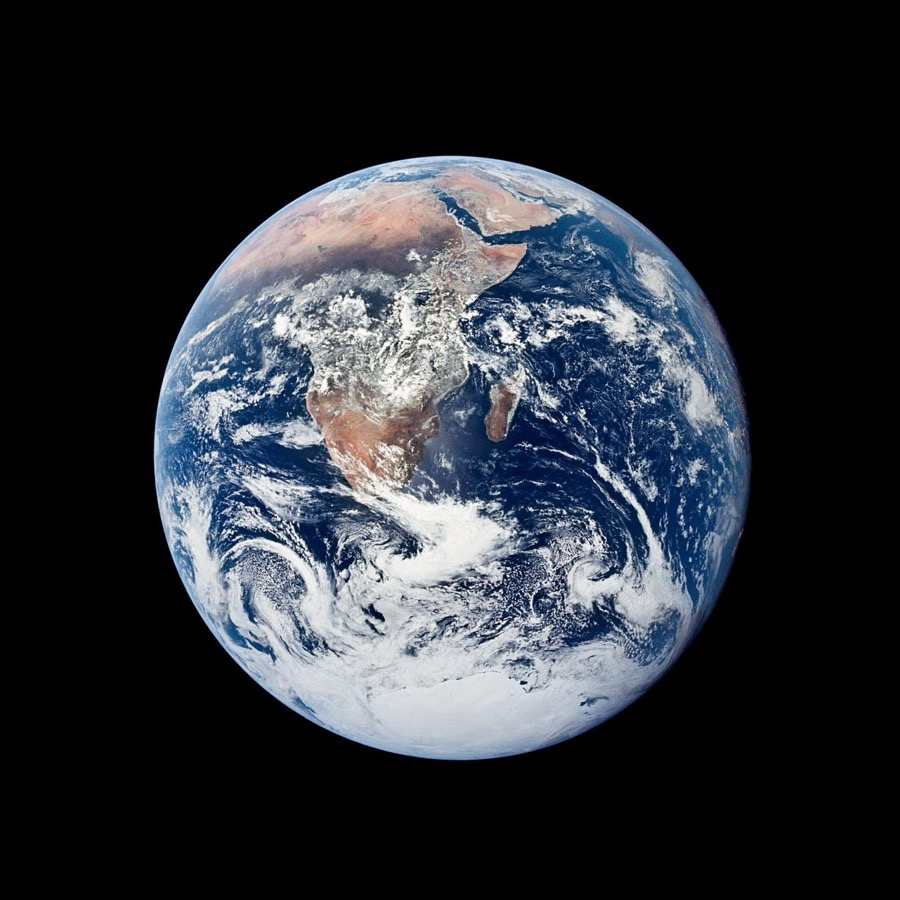
\includegraphics[width=0.55\linewidth]{images/blue-marble-nasa.jpg}
  \caption{Beispielabbildung mit Quellenangabe~\cite{nasa-blue-marble}}
  \label{abb:blue-marble}
\end{figure}

Vektorgrafiken haben gegenüber Screenshots den Vorteil, dass

\begin{itemize}
  \item sie jederzeit editiert werden können,
  \item sie beliebig skaliert werden können, ohne unscharf zu werden,
  \item alle Grafiken einheitlich vergrößert oder verkleinert werden können.
        Das verbessert das Layout ungemein.
\end{itemize}

Abbildungen stehen immer alleinstehend und zentriert. Die Breite wird
relativ zur Textbreite angegeben (\lstinline|width=0.75\linewidth|), damit
sie nie über den Satzspiegel hinausragt. Sollen mehrere Grafiken
nebeneinander stehen, verwendet dafür zwei \lstinline|minipage|-Umgebungen
innerhalb einer \lstinline|figure|.

Die Positionierung übernimmt \LaTeX. Die Angabe \lstinline|[htbp]| erlaubt
es, die Abbildung an die Stelle im Text, an den Seitenanfang, an das
Seitenende oder auf eine eigene Seite zu setzen. Eine Abbildung kann dadurch
auf der Folgeseite landen -- das ist beabsichtigt und kein Fehler.

\subsection{Beschriftungen}

Alle Grafiken und Tabellen sind zu beschriften und mit Quellenangaben zu
versehen. Im Text muss auf jede Abbildung und jede Tabelle Bezug genommen
werden.

Die Beschriftung erfolgt mit \lstinline|\caption| innerhalb der
\lstinline|figure|- bzw.\ \lstinline|table|-Umgebung. Nur so werden
Abbildungs- und Tabellenverzeichnis korrekt geführt. Bei Abbildungen steht
die Beschriftung unter der Grafik, bei Tabellen darüber; die Vorlage stellt
das automatisch richtig ein.

Abbildungen werden mit \enquote{Abb.} und Tabellen mit \enquote{Tab.}
bezeichnet. Auch das erledigt die Vorlage; die Nummerierung läuft
durchgehend und nicht kapitelweise. In englischsprachigen Diplomarbeiten
wird \enquote{Abb.} durch \enquote{Fig.} ersetzt -- dafür genügt die
Klassenoption \lstinline|englisch|.

Unmittelbar nach \lstinline|\caption| gehört ein \lstinline|\label|. Ohne
Label lässt sich die Abbildung später nicht referenzieren. Bewährt hat sich
ein Präfix je Objektart: \lstinline|abb:|, \lstinline|tab:| und
\lstinline|code:|.

\subsection{Querverweise}

Textpassagen, die sich auf andere Kapitel, Grafiken oder Tabellen beziehen,
müssen eine Referenz enthalten. Diese wird mit \lstinline|\ref| erzeugt und
enthält zumindest die Kategorie und die Nummer, also etwa
\lstinline|Abb.~\ref{abb:aufbau}|. Das geschützte Leerzeichen
\lstinline|~| verhindert, dass zwischen Bezeichnung und Nummer umgebrochen
wird.

Liegen referenzierender Text und referenziertes Objekt mehr als eine Seite
auseinander, ist zusätzlich die Seitenzahl mit \lstinline|\pageref|
anzugeben.

Anders als in Word müssen Querverweise und Verzeichnisse nicht manuell
aktualisiert werden. \LaTeX{} löst sie beim Übersetzen auf, benötigt dafür
aber mehrere Durchläufe. \lstinline|latexmk| (bzw.\ \lstinline|make pdf|)
wiederholt den Lauf so lange, bis sich nichts mehr ändert. Meldet das
Protokoll am Ende \enquote{There were undefined references}, fehlt ein
\lstinline|\label| oder es ist falsch geschrieben.

\subsection{Quellenangaben}

In wissenschaftlichen Arbeiten ist es verpflichtend, die Quelle jeder
Aussage anzugeben, die nicht von einem selbst stammt. Der Leser muss die
Möglichkeit haben, die Ausführungen des Autors nachzuprüfen.

Zu diesem Zweck müssen im Text der Diplomarbeit alle verwendeten Quellen
(Fachbücher, Fachzeitschriften, Herstellerunterlagen, Webseiten, \ldots)
angegeben werden. Dies geschieht am Ende des zitierten Textes durch Angabe
der Quelle. Informationen aus Lehrbüchern können als Allgemeinwissen
vorausgesetzt werden und müssen nicht zitiert werden.

Bei inhaltlichen Zitaten, dem Normalfall in technischen Arbeiten, wird der
Inhalt der Quelle nur sinngemäß wiedergegeben.

Bei wörtlichen Zitaten, die in technischen Arbeiten eher selten auftreten,
wird die wörtlich zitierte Textstelle zwischen Anführungszeichen gesetzt,
dahinter steht die Quellenangabe. Eigene Kommentare im Zitat oder
Verkürzungen werden in eckigen Klammern angegeben. Kurze Zitate stehen mit
\lstinline|\zitat| im Fließtext, längere in der Umgebung
\lstinline|zitatfreistehend|.

Beispiel für ein Zitat im Text der Diplomarbeit:
\zitat{[\ldots] kann in diesem Fall eine relationale Datenbank vorteilhaft
eingesetzt werden}~\cite{beispiel-buch}.

Beispiel für ein Zitat als eigener Absatz:

\begin{zitatfreistehend}
  \enquote{The basic guideline for citing online sources is to follow the
  standard citation for the citation, or add the DOI in place of page
  numbers if the source is not paginated.}~\cite{beispiel-artikel}
\end{zitatfreistehend}

Für Diplomarbeiten an der \ac{HTL} Donaustadt ist der IEEE-Zitierstil zu
verwenden. Jeder Quelle wird eine Nummer zugeordnet und in eckigen Klammern
angegeben. Diese Vorlage stellt den Stil bereits ein; zitiert wird mit
\lstinline|\cite{schluessel}|, wobei der Schlüssel aus
\lstinline|references.bib| stammt. Das Quellenverzeichnis wird daraus
automatisch erzeugt und enthält nur tatsächlich zitierte Einträge.

Zum Verwalten der Quellen empfiehlt sich Zotero mit dem Plug-in Better
BibTeX, das \lstinline|references.bib| bei jeder Änderung automatisch neu
exportiert.

Es gibt viele verschiedene Typen von Quellen. Tab.~\ref{tab:quellentypen}
zeigt die häufigsten, den passenden BibTeX-Eintragstyp und die
Informationen, die mindestens enthalten sein sollten.

\begin{table}[htbp]
  \centering
  \caption{Quellentypen}
  \label{tab:quellentypen}
  \begin{tabular}{@{}p{0.28\linewidth}p{0.16\linewidth}p{0.46\linewidth}@{}}
    \toprule
    \tabkopf{Quellentyp} & \tabkopf{Eintragstyp} &
      \tabkopf{wichtigste Informationen} \\
    \midrule
    Buch (auch E-Books, Broschüren) & \lstinline|@book| &
      Autor(en), Titel, Auflage, Verlag, Ort, ISBN \\
    Diplomarbeit, Dissertation & \lstinline|@thesis| &
      Autor(en), Titel, Institution, Ort, Datum \\
    Webseite (auch PDF) & \lstinline|@online| &
      Autor(en), Titel, URL, Abrufdatum (\lstinline|urldate|) \\
    Zeitschriftenartikel & \lstinline|@article| &
      Autor(en), Titel, Publikation, Band, Ausgabe, Seiten, Datum \\
    Verwendung von KI & \lstinline|@online| &
      siehe Anhang und die Vorgaben des Ministeriums~\cite{beispiel-online} \\
    \bottomrule
  \end{tabular}
\end{table}

\subsection{Befehle und Umgebungen}

In Word übernehmen Formatvorlagen das einheitliche Layout. In \LaTeX{}
erfüllen Befehle und Umgebungen dieselbe Aufgabe: Der Text beschreibt, was
etwas \emph{ist}, das Aussehen legt die Dokumentklasse \lstinline|htldon.cls|
zentral fest. Dadurch lässt sich die Formatierung nachträglich an einer
einzigen Stelle ändern.

Die in Tab.~\ref{tab:befehle} aufgeführten Befehle stellen sicher, dass alle
Diplomarbeiten den Richtlinien entsprechen. Sie dürfen nur in begründeten
Ausnahmefällen angepasst werden.

\begin{table}[htbp]
  \centering
  \caption{Befehle und Umgebungen der Vorlage}
  \label{tab:befehle}
  \begin{tabular}{@{}p{0.36\linewidth}p{0.58\linewidth}@{}}
    \toprule
    \tabkopf{Befehl} & \tabkopf{Beschreibung} \\
    \midrule
    \lstinline|\chapter| bis \lstinline|\subsubsection| &
      Kapitelüberschriften mit Dezimalklassifikation. Die ersten drei Ebenen
      erscheinen im Inhaltsverzeichnis, \lstinline|\subsubsection| nicht. \\
    \lstinline|\paragraph| &
      Zwischenüberschrift ohne Nummerierung, nicht im Inhaltsverzeichnis. \\
    \lstinline|\abschnittsautor| &
      Verfasser/in eines Abschnitts, erscheint rechts in der Kopfzeile.
      Format: erster Buchstabe des Vornamens, Punkt, Nachname
      (\enquote{M. Muster}). \\
    \lstinline|\zitat|, \lstinline|zitatfreistehend| &
      Kennzeichnung wörtlicher Zitate im Fließtext bzw.\ als eigener Absatz. \\
    \lstinline|\menue| &
      Menüstrukturen (\menue{Datei / Öffnen}) und Tastatureingaben
      (\menue{Strg + A}). \\
    \lstinline|lstlisting|, \lstinline|\lstinline| &
      Quellcode als eigener Block bzw.\ im Fließtext. \\
    \lstinline|\tabkopf| &
      Kopfzeile einer Tabelle. Der Tabelleninhalt selbst wird von der Klasse
      automatisch auf 10\,pt und linksbündig gestellt. \\
    \lstinline|\ac|, \lstinline|\acp| &
      Abkürzung, beim ersten Auftreten ausgeschrieben, im Plural mit
      \lstinline|\acp|. \\
    \lstinline|\cite|, \lstinline|\ref|, \lstinline|\pageref| &
      Quellenangabe, Querverweis, Seitenverweis. \\
    \bottomrule
  \end{tabular}
\end{table}

Überschriften der Kapitel müssen kurz, präzise und selbsterklärend sein.
Beispiele für unzureichende Überschriften: \enquote{5.3 Aufbau},
\enquote{5.3 Messergebnis}, \enquote{5.3 Beispiel}.

Bei Unterüberschriften gilt:

\begin{itemize}
  \item Es muss mindestens zwei Unterpunkte geben. Ein Abschnitt 3.2.1 darf
        daher nicht existieren, wenn kein 3.2.2 folgt.
  \item Unterpunkte sollten inhaltlich ausreichend gefüllt sein und
        mindestens eine halbe Seite umfassen.
  \item Unterpunkte, die lediglich aus einem einzelnen Satz bestehen, werden
        besser als Aufzählung dargestellt.
\end{itemize}

Für die Darstellung von Quellcode gilt:

\begin{itemize}
  \item Umfang:
        \begin{itemize}
          \item Der vollständige Sourcecode gehört ausschließlich auf das
                elektronische Speichermedium.
          \item Im Dokument selbst sollen nur wesentliche Ausschnitte
                aufgenommen werden.
        \end{itemize}
  \item Formatierung: Schriftart und Schriftgröße gibt die
        \lstinline|lstlisting|-Umgebung vor, der Zeilenabstand ist dort
        einzeilig. Die Sprache wird mit
        \lstinline|[language=Python]| angegeben, damit die
        Syntaxhervorhebung stimmt.
  \item Inhaltliche Anforderungen: Der Sourcecode muss ausreichend
        kommentiert sein.
  \item Verwendung im Fließtext: Wird Sourcecode im Text erwähnt, ist
        \lstinline|\lstinline| zu verwenden. Zusätzliche Anführungszeichen
        sind nicht erforderlich. Beispiel: Mit dem Befehl
        \lstinline|ShowModal| wird ein Frame geöffnet.
\end{itemize}

\section{Beschreibung der Kapitel}

\subsection{Titelseite}

Die Titelseite wird vollständig aus \lstinline|metadata.tex| erzeugt. Dort
sind einzutragen:

\begin{itemize}
  \item der Titel der Diplomarbeit mit \lstinline|\titel|. Er wird
        automatisch in die Kopfzeile übernommen.
  \item ein Projektlogo, Bild oder eine Zeichnung mit
        \lstinline|\projektlogo|.
  \item alle Verfasser/innen mit \lstinline|\teammitglied| und die
        Betreuung mit \lstinline|\betreuung|.
  \item Schuljahr, Abteilung und Klasse.
\end{itemize}

Falls alle Verfasser/innen oder Betreuer/innen dasselbe Geschlecht haben,
kann die geschlechtsspezifische Form verwendet werden; dafür ist das
optionale Argument von \lstinline|\betreuung| vorgesehen.

\subsection{Verfassererklärung}

In der Verfassererklärung bekennen sich die Verfasser/innen zu einem
wissenschaftlichen Arbeitsstil. Sollten im Nachhinein grobe Verstöße dagegen
aufgedeckt werden, kann die Arbeit für ungültig erklärt und der Abschluss
revidiert werden.

Die Erklärung erzeugt \lstinline|\eigenstaendigkeitserklaerung|. Je
Teammitglied entsteht automatisch eine Unterschriftszeile. Zu ergänzen sind
gegebenenfalls Kooperationen mit Firmen und Sperrvermerke.

\subsection{Problemstellung}

Die Seite \enquote{Problemstellung} wird durch den eingescannten Antrag (mit
allen Stempeln und Unterschriften) vollflächig ersetzt. Dazu wird in
\lstinline|frontmatter/problem-statement.tex| das Scan-PDF eingebunden.

\subsection{Kurzfassung bzw.\ Abstract}

Die Kurzfassung bzw.\ der Abstract soll kurz, prägnant und verständlich den
Inhalt der Arbeit wiedergeben: Zielsetzung, Ablauf, wichtigste Erkenntnisse,
wesentliche Merkmale des realisierten Produkts, Schlussfolgerungen und
Ausblick. Beide sind als eigenständiges Dokument zu konzipieren, das
unabhängig von der Diplomarbeit gelesen und verstanden werden kann, und
sollen in Deutsch und Englisch jeweils nicht mehr als eine Seite umfassen.

\subsection{Inhaltsverzeichnis}

Das Inhaltsverzeichnis wird automatisch aus den Überschriften erstellt. Es
zeigt die ersten drei Ebenen, der Text steht linksbündig, die Seitenzahlen
rechtsbündig, als Füllzeichen dienen Punkte. Eine manuelle Aktualisierung
ist nicht nötig.

\subsection{Die weiteren Kapitel}

Die Kapitel Projektplanung, Technische Grundlagen, Praktische Realisierung
sowie Evaluierung und Ergebnisse beschreiben die Diplomarbeit im Detail.

Für die Beurteilung ist es wichtig, den/die Verfasser/in zu kennen. Daher
ist dieser Hinweis auf jeder Seite rechtsbündig in der Kopfzeile zu
vermerken. Dafür wird \lstinline|\abschnittsautor| direkt nach der
Überschrift gesetzt; der Eintrag gilt ab dort bis zur nächsten Angabe.
Haben mehrere Personen gemeinsam an einem Abschnitt gearbeitet, sind alle zu
nennen, durch Komma getrennt:
\lstinline|\abschnittsautor{A. Erste, B. Zweite}|.

Die Projektplanung soll die systematische Durchführung der Diplomarbeit
innerhalb des Projektteams beschreiben. Dabei sollen geplante Ziele und
tatsächlich erreichte Ergebnisse miteinander verglichen und die Unterschiede
reflektiert werden. Beim klassischen Wasserfall-Projektmanagement können
etwa die Meilensteine als Referenz dienen, bei agiler Projektorganisation
die Sprint-Reviews.

Im Kapitel Technische Grundlagen finden sich alle für das unmittelbare
technische Verständnis der Diplomarbeit relevanten Inhalte. Hier wird
insbesondere auf korrekte Zitate und den sorgfältigen Einsatz von Quellen
geachtet.

Das Kapitel Praktische Realisierung enthält die praktischen Eigenleistungen
der Diplomarbeit. Dabei sollen die Vorgänge und Untersuchungen beschrieben
und nachvollziehbar dokumentiert werden.

Im Kapitel Evaluierung und Ergebnisse erfolgt die Darstellung und Bewertung
der abschließenden Arbeit. Hier soll ebenso, sofern vorhanden, das
Endprodukt bzw.\ der Prototyp präsentiert und beschrieben werden.

\subsection{Anhang}

Im Anhang können alle Informationen gesammelt werden, die zwar zur
Diplomarbeit gehören, jedoch im Inhaltsteil den Rahmen gesprengt hätten.
Dazu zählen wichtige Notizen (z.\,B. Gesprächsprotokolle), Normen,
Schnittstellendefinitionen oder Präsentationen. Weiters soll der Anhang den
Inhalt eines beigefügten elektronischen Speichermediums sowie einen
einseitigen Lebenslauf jedes Teammitglieds enthalten.

Verpflichtend ist außerdem die Dokumentation aller eingesetzten KI-basierten
Hilfsmittel. Dafür ist \lstinline|appendix/ai-tools.tex| vorgesehen.
| zu löschen. Die Einträge
im Inhaltsverzeichnis und in den übrigen Verzeichnissen verschwinden beim
nächsten Übersetzen von selbst.

\subsection{Abgabe der Diplomarbeit}

Die Diplomarbeit ist in gedruckter bzw.\ gebundener Form und in digitaler
Form vorzulegen. Dem Abteilungsvorstand sind zwei geheftete Exemplare (ein
Belegexemplar und ein Beurteilungsexemplar für den/die Betreuer/in) zu
übergeben.

Nach erfolgter Beurteilung geht das Beurteilungsexemplar temporär zurück an
die Diplomarbeitsgruppe. Nun können letzte Korrekturen (ohne
Beurteilungsrelevanz) vorgenommen werden. Anschließend wird die Arbeit erneut
ausgedruckt und gesammelt zur Bindung außer Haus gegeben. Weitere Exemplare
für Kooperationspartner (Firmen, Institutionen) oder Projektteilnehmer können
in diesem Zusammenhang erstellt werden.

\subsection{Grafiken}

Abbildungen müssen in gut lesbarer Bildqualität eingefügt werden. Grafiken
sollten am besten in einem vektorbasierten Zeichenprogramm (z.\,B. Inkscape,
draw.io) erstellt und als PDF exportiert werden; PDF und PNG lassen sich
direkt einbinden, SVG nicht. Alle Bilddateien gehören in den Ordner
\lstinline|images/|.

\begin{lstlisting}[language={[LaTeX]TeX}, caption={Eine Abbildung einbinden},
                   label=code:abbildung]
\begin{figure}[htbp]
  \centering
  
\includegraphics[width=0.75\linewidth]{images/example-figure.pdf}
  \caption{Aufbau des Systems}
  \label{abb:aufbau}
\end{figure}
\end{lstlisting}

Abb.~\ref{abb:blue-marble} zeigt, wie das Ergebnis aussieht. Stammt die
Grafik nicht von euch selbst, gehört die Quelle in die Beschriftung.

\begin{figure}[htbp]
  \centering
  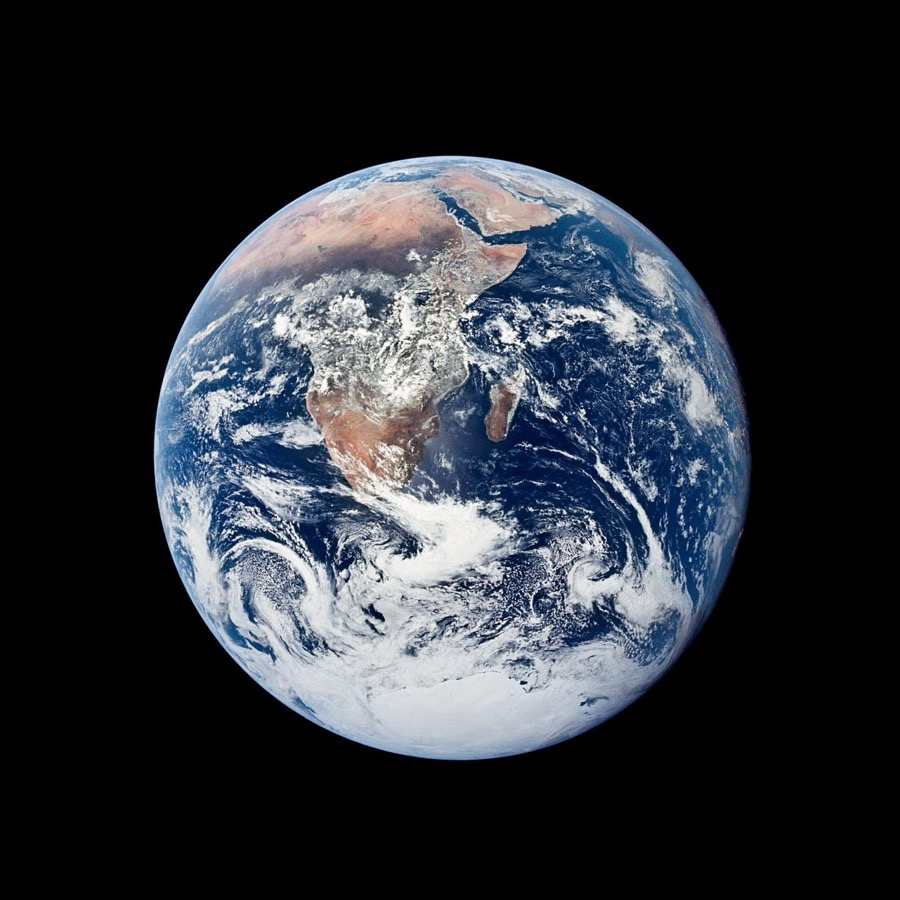
\includegraphics[width=0.55\linewidth]{images/blue-marble-nasa.jpg}
  \caption{Beispielabbildung mit Quellenangabe~\cite{nasa-blue-marble}}
  \label{abb:blue-marble}
\end{figure}

Vektorgrafiken haben gegenüber Screenshots den Vorteil, dass

\begin{itemize}
  \item sie jederzeit editiert werden können,
  \item sie beliebig skaliert werden können, ohne unscharf zu werden,
  \item alle Grafiken einheitlich vergrößert oder verkleinert werden können.
        Das verbessert das Layout ungemein.
\end{itemize}

Abbildungen stehen immer alleinstehend und zentriert. Die Breite wird
relativ zur Textbreite angegeben (\lstinline|width=0.75\linewidth|), damit
sie nie über den Satzspiegel hinausragt. Sollen mehrere Grafiken
nebeneinander stehen, verwendet dafür zwei \lstinline|minipage|-Umgebungen
innerhalb einer \lstinline|figure|.

Die Positionierung übernimmt \LaTeX. Die Angabe \lstinline|[htbp]| erlaubt
es, die Abbildung an die Stelle im Text, an den Seitenanfang, an das
Seitenende oder auf eine eigene Seite zu setzen. Eine Abbildung kann dadurch
auf der Folgeseite landen -- das ist beabsichtigt und kein Fehler.

\subsection{Beschriftungen}

Alle Grafiken und Tabellen sind zu beschriften und mit Quellenangaben zu
versehen. Im Text muss auf jede Abbildung und jede Tabelle Bezug genommen
werden.

Die Beschriftung erfolgt mit \lstinline|\caption| innerhalb der
\lstinline|figure|- bzw.\ \lstinline|table|-Umgebung. Nur so werden
Abbildungs- und Tabellenverzeichnis korrekt geführt. Bei Abbildungen steht
die Beschriftung unter der Grafik, bei Tabellen darüber; die Vorlage stellt
das automatisch richtig ein.

Abbildungen werden mit \enquote{Abb.} und Tabellen mit \enquote{Tab.}
bezeichnet. Auch das erledigt die Vorlage; die Nummerierung läuft
durchgehend und nicht kapitelweise. In englischsprachigen Diplomarbeiten
wird \enquote{Abb.} durch \enquote{Fig.} ersetzt -- dafür genügt die
Klassenoption \lstinline|englisch|.

Unmittelbar nach \lstinline|\caption| gehört ein \lstinline|\label|. Ohne
Label lässt sich die Abbildung später nicht referenzieren. Bewährt hat sich
ein Präfix je Objektart: \lstinline|abb:|, \lstinline|tab:| und
\lstinline|code:|.

\subsection{Querverweise}

Textpassagen, die sich auf andere Kapitel, Grafiken oder Tabellen beziehen,
müssen eine Referenz enthalten. Diese wird mit \lstinline|\ref| erzeugt und
enthält zumindest die Kategorie und die Nummer, also etwa
\lstinline|Abb.~\ref{abb:aufbau}|. Das geschützte Leerzeichen
\lstinline|~| verhindert, dass zwischen Bezeichnung und Nummer umgebrochen
wird.

Liegen referenzierender Text und referenziertes Objekt mehr als eine Seite
auseinander, ist zusätzlich die Seitenzahl mit \lstinline|\pageref|
anzugeben.

Anders als in Word müssen Querverweise und Verzeichnisse nicht manuell
aktualisiert werden. \LaTeX{} löst sie beim Übersetzen auf, benötigt dafür
aber mehrere Durchläufe. \lstinline|latexmk| (bzw.\ \lstinline|make pdf|)
wiederholt den Lauf so lange, bis sich nichts mehr ändert. Meldet das
Protokoll am Ende \enquote{There were undefined references}, fehlt ein
\lstinline|\label| oder es ist falsch geschrieben.

\subsection{Quellenangaben}

In wissenschaftlichen Arbeiten ist es verpflichtend, die Quelle jeder
Aussage anzugeben, die nicht von einem selbst stammt. Der Leser muss die
Möglichkeit haben, die Ausführungen des Autors nachzuprüfen.

Zu diesem Zweck müssen im Text der Diplomarbeit alle verwendeten Quellen
(Fachbücher, Fachzeitschriften, Herstellerunterlagen, Webseiten, \ldots)
angegeben werden. Dies geschieht am Ende des zitierten Textes durch Angabe
der Quelle. Informationen aus Lehrbüchern können als Allgemeinwissen
vorausgesetzt werden und müssen nicht zitiert werden.

Bei inhaltlichen Zitaten, dem Normalfall in technischen Arbeiten, wird der
Inhalt der Quelle nur sinngemäß wiedergegeben.

Bei wörtlichen Zitaten, die in technischen Arbeiten eher selten auftreten,
wird die wörtlich zitierte Textstelle zwischen Anführungszeichen gesetzt,
dahinter steht die Quellenangabe. Eigene Kommentare im Zitat oder
Verkürzungen werden in eckigen Klammern angegeben. Kurze Zitate stehen mit
\lstinline|\zitat| im Fließtext, längere in der Umgebung
\lstinline|zitatfreistehend|.

Beispiel für ein Zitat im Text der Diplomarbeit:
\zitat{[\ldots] kann in diesem Fall eine relationale Datenbank vorteilhaft
eingesetzt werden}~\cite{beispiel-buch}.

Beispiel für ein Zitat als eigener Absatz:

\begin{zitatfreistehend}
  \enquote{The basic guideline for citing online sources is to follow the
  standard citation for the citation, or add the DOI in place of page
  numbers if the source is not paginated.}~\cite{beispiel-artikel}
\end{zitatfreistehend}

Für Diplomarbeiten an der \ac{HTL} Donaustadt ist der IEEE-Zitierstil zu
verwenden. Jeder Quelle wird eine Nummer zugeordnet und in eckigen Klammern
angegeben. Diese Vorlage stellt den Stil bereits ein; zitiert wird mit
\lstinline|\cite{schluessel}|, wobei der Schlüssel aus
\lstinline|references.bib| stammt. Das Quellenverzeichnis wird daraus
automatisch erzeugt und enthält nur tatsächlich zitierte Einträge.

Zum Verwalten der Quellen empfiehlt sich Zotero mit dem Plug-in Better
BibTeX, das \lstinline|references.bib| bei jeder Änderung automatisch neu
exportiert.

Es gibt viele verschiedene Typen von Quellen. Tab.~\ref{tab:quellentypen}
zeigt die häufigsten, den passenden BibTeX-Eintragstyp und die
Informationen, die mindestens enthalten sein sollten.

\begin{table}[htbp]
  \centering
  \caption{Quellentypen}
  \label{tab:quellentypen}
  \begin{tabular}{@{}p{0.28\linewidth}p{0.16\linewidth}p{0.46\linewidth}@{}}
    \toprule
    \tabkopf{Quellentyp} & \tabkopf{Eintragstyp} &
      \tabkopf{wichtigste Informationen} \\
    \midrule
    Buch (auch E-Books, Broschüren) & \lstinline|@book| &
      Autor(en), Titel, Auflage, Verlag, Ort, ISBN \\
    Diplomarbeit, Dissertation & \lstinline|@thesis| &
      Autor(en), Titel, Institution, Ort, Datum \\
    Webseite (auch PDF) & \lstinline|@online| &
      Autor(en), Titel, URL, Abrufdatum (\lstinline|urldate|) \\
    Zeitschriftenartikel & \lstinline|@article| &
      Autor(en), Titel, Publikation, Band, Ausgabe, Seiten, Datum \\
    Verwendung von KI & \lstinline|@online| &
      siehe Anhang und die Vorgaben des Ministeriums~\cite{beispiel-online} \\
    \bottomrule
  \end{tabular}
\end{table}

\subsection{Befehle und Umgebungen}

In Word übernehmen Formatvorlagen das einheitliche Layout. In \LaTeX{}
erfüllen Befehle und Umgebungen dieselbe Aufgabe: Der Text beschreibt, was
etwas \emph{ist}, das Aussehen legt die Dokumentklasse \lstinline|htldon.cls|
zentral fest. Dadurch lässt sich die Formatierung nachträglich an einer
einzigen Stelle ändern.

Die in Tab.~\ref{tab:befehle} aufgeführten Befehle stellen sicher, dass alle
Diplomarbeiten den Richtlinien entsprechen. Sie dürfen nur in begründeten
Ausnahmefällen angepasst werden.

\begin{table}[htbp]
  \centering
  \caption{Befehle und Umgebungen der Vorlage}
  \label{tab:befehle}
  \begin{tabular}{@{}p{0.36\linewidth}p{0.58\linewidth}@{}}
    \toprule
    \tabkopf{Befehl} & \tabkopf{Beschreibung} \\
    \midrule
    \lstinline|\chapter| bis \lstinline|\subsubsection| &
      Kapitelüberschriften mit Dezimalklassifikation. Die ersten drei Ebenen
      erscheinen im Inhaltsverzeichnis, \lstinline|\subsubsection| nicht. \\
    \lstinline|\paragraph| &
      Zwischenüberschrift ohne Nummerierung, nicht im Inhaltsverzeichnis. \\
    \lstinline|\abschnittsautor| &
      Verfasser/in eines Abschnitts, erscheint rechts in der Kopfzeile.
      Format: erster Buchstabe des Vornamens, Punkt, Nachname
      (\enquote{M. Muster}). \\
    \lstinline|\zitat|, \lstinline|zitatfreistehend| &
      Kennzeichnung wörtlicher Zitate im Fließtext bzw.\ als eigener Absatz. \\
    \lstinline|\menue| &
      Menüstrukturen (\menue{Datei / Öffnen}) und Tastatureingaben
      (\menue{Strg + A}). \\
    \lstinline|lstlisting|, \lstinline|\lstinline| &
      Quellcode als eigener Block bzw.\ im Fließtext. \\
    \lstinline|\tabkopf| &
      Kopfzeile einer Tabelle. Der Tabelleninhalt selbst wird von der Klasse
      automatisch auf 10\,pt und linksbündig gestellt. \\
    \lstinline|\ac|, \lstinline|\acp| &
      Abkürzung, beim ersten Auftreten ausgeschrieben, im Plural mit
      \lstinline|\acp|. \\
    \lstinline|\cite|, \lstinline|\ref|, \lstinline|\pageref| &
      Quellenangabe, Querverweis, Seitenverweis. \\
    \bottomrule
  \end{tabular}
\end{table}

Überschriften der Kapitel müssen kurz, präzise und selbsterklärend sein.
Beispiele für unzureichende Überschriften: \enquote{5.3 Aufbau},
\enquote{5.3 Messergebnis}, \enquote{5.3 Beispiel}.

Bei Unterüberschriften gilt:

\begin{itemize}
  \item Es muss mindestens zwei Unterpunkte geben. Ein Abschnitt 3.2.1 darf
        daher nicht existieren, wenn kein 3.2.2 folgt.
  \item Unterpunkte sollten inhaltlich ausreichend gefüllt sein und
        mindestens eine halbe Seite umfassen.
  \item Unterpunkte, die lediglich aus einem einzelnen Satz bestehen, werden
        besser als Aufzählung dargestellt.
\end{itemize}

Für die Darstellung von Quellcode gilt:

\begin{itemize}
  \item Umfang:
        \begin{itemize}
          \item Der vollständige Sourcecode gehört ausschließlich auf das
                elektronische Speichermedium.
          \item Im Dokument selbst sollen nur wesentliche Ausschnitte
                aufgenommen werden.
        \end{itemize}
  \item Formatierung: Schriftart und Schriftgröße gibt die
        \lstinline|lstlisting|-Umgebung vor, der Zeilenabstand ist dort
        einzeilig. Die Sprache wird mit
        \lstinline|[language=Python]| angegeben, damit die
        Syntaxhervorhebung stimmt.
  \item Inhaltliche Anforderungen: Der Sourcecode muss ausreichend
        kommentiert sein.
  \item Verwendung im Fließtext: Wird Sourcecode im Text erwähnt, ist
        \lstinline|\lstinline| zu verwenden. Zusätzliche Anführungszeichen
        sind nicht erforderlich. Beispiel: Mit dem Befehl
        \lstinline|ShowModal| wird ein Frame geöffnet.
\end{itemize}

\section{Beschreibung der Kapitel}

\subsection{Titelseite}

Die Titelseite wird vollständig aus \lstinline|metadata.tex| erzeugt. Dort
sind einzutragen:

\begin{itemize}
  \item der Titel der Diplomarbeit mit \lstinline|\titel|. Er wird
        automatisch in die Kopfzeile übernommen.
  \item ein Projektlogo, Bild oder eine Zeichnung mit
        \lstinline|\projektlogo|.
  \item alle Verfasser/innen mit \lstinline|\teammitglied| und die
        Betreuung mit \lstinline|\betreuung|.
  \item Schuljahr, Abteilung und Klasse.
\end{itemize}

Falls alle Verfasser/innen oder Betreuer/innen dasselbe Geschlecht haben,
kann die geschlechtsspezifische Form verwendet werden; dafür ist das
optionale Argument von \lstinline|\betreuung| vorgesehen.

\subsection{Verfassererklärung}

In der Verfassererklärung bekennen sich die Verfasser/innen zu einem
wissenschaftlichen Arbeitsstil. Sollten im Nachhinein grobe Verstöße dagegen
aufgedeckt werden, kann die Arbeit für ungültig erklärt und der Abschluss
revidiert werden.

Die Erklärung erzeugt \lstinline|\eigenstaendigkeitserklaerung|. Je
Teammitglied entsteht automatisch eine Unterschriftszeile. Zu ergänzen sind
gegebenenfalls Kooperationen mit Firmen und Sperrvermerke.

\subsection{Problemstellung}

Die Seite \enquote{Problemstellung} wird durch den eingescannten Antrag (mit
allen Stempeln und Unterschriften) vollflächig ersetzt. Dazu wird in
\lstinline|frontmatter/problem-statement.tex| das Scan-PDF eingebunden.

\subsection{Kurzfassung bzw.\ Abstract}

Die Kurzfassung bzw.\ der Abstract soll kurz, prägnant und verständlich den
Inhalt der Arbeit wiedergeben: Zielsetzung, Ablauf, wichtigste Erkenntnisse,
wesentliche Merkmale des realisierten Produkts, Schlussfolgerungen und
Ausblick. Beide sind als eigenständiges Dokument zu konzipieren, das
unabhängig von der Diplomarbeit gelesen und verstanden werden kann, und
sollen in Deutsch und Englisch jeweils nicht mehr als eine Seite umfassen.

\subsection{Inhaltsverzeichnis}

Das Inhaltsverzeichnis wird automatisch aus den Überschriften erstellt. Es
zeigt die ersten drei Ebenen, der Text steht linksbündig, die Seitenzahlen
rechtsbündig, als Füllzeichen dienen Punkte. Eine manuelle Aktualisierung
ist nicht nötig.

\subsection{Die weiteren Kapitel}

Die Kapitel Projektplanung, Technische Grundlagen, Praktische Realisierung
sowie Evaluierung und Ergebnisse beschreiben die Diplomarbeit im Detail.

Für die Beurteilung ist es wichtig, den/die Verfasser/in zu kennen. Daher
ist dieser Hinweis auf jeder Seite rechtsbündig in der Kopfzeile zu
vermerken. Dafür wird \lstinline|\abschnittsautor| direkt nach der
Überschrift gesetzt; der Eintrag gilt ab dort bis zur nächsten Angabe.
Haben mehrere Personen gemeinsam an einem Abschnitt gearbeitet, sind alle zu
nennen, durch Komma getrennt:
\lstinline|\abschnittsautor{A. Erste, B. Zweite}|.

Die Projektplanung soll die systematische Durchführung der Diplomarbeit
innerhalb des Projektteams beschreiben. Dabei sollen geplante Ziele und
tatsächlich erreichte Ergebnisse miteinander verglichen und die Unterschiede
reflektiert werden. Beim klassischen Wasserfall-Projektmanagement können
etwa die Meilensteine als Referenz dienen, bei agiler Projektorganisation
die Sprint-Reviews.

Im Kapitel Technische Grundlagen finden sich alle für das unmittelbare
technische Verständnis der Diplomarbeit relevanten Inhalte. Hier wird
insbesondere auf korrekte Zitate und den sorgfältigen Einsatz von Quellen
geachtet.

Das Kapitel Praktische Realisierung enthält die praktischen Eigenleistungen
der Diplomarbeit. Dabei sollen die Vorgänge und Untersuchungen beschrieben
und nachvollziehbar dokumentiert werden.

Im Kapitel Evaluierung und Ergebnisse erfolgt die Darstellung und Bewertung
der abschließenden Arbeit. Hier soll ebenso, sofern vorhanden, das
Endprodukt bzw.\ der Prototyp präsentiert und beschrieben werden.

\subsection{Anhang}

Im Anhang können alle Informationen gesammelt werden, die zwar zur
Diplomarbeit gehören, jedoch im Inhaltsteil den Rahmen gesprengt hätten.
Dazu zählen wichtige Notizen (z.\,B. Gesprächsprotokolle), Normen,
Schnittstellendefinitionen oder Präsentationen. Weiters soll der Anhang den
Inhalt eines beigefügten elektronischen Speichermediums sowie einen
einseitigen Lebenslauf jedes Teammitglieds enthalten.

Verpflichtend ist außerdem die Dokumentation aller eingesetzten KI-basierten
Hilfsmittel. Dafür ist \lstinline|appendix/ai-tools.tex| vorgesehen.
| zu löschen. Die Einträge
im Inhaltsverzeichnis und in den übrigen Verzeichnissen verschwinden beim
nächsten Übersetzen von selbst.

\subsection{Abgabe der Diplomarbeit}

Die Diplomarbeit ist in gedruckter bzw.\ gebundener Form und in digitaler
Form vorzulegen. Dem Abteilungsvorstand sind zwei geheftete Exemplare (ein
Belegexemplar und ein Beurteilungsexemplar für den/die Betreuer/in) zu
übergeben.

Nach erfolgter Beurteilung geht das Beurteilungsexemplar temporär zurück an
die Diplomarbeitsgruppe. Nun können letzte Korrekturen (ohne
Beurteilungsrelevanz) vorgenommen werden. Anschließend wird die Arbeit erneut
ausgedruckt und gesammelt zur Bindung außer Haus gegeben. Weitere Exemplare
für Kooperationspartner (Firmen, Institutionen) oder Projektteilnehmer können
in diesem Zusammenhang erstellt werden.

\subsection{Grafiken}

Abbildungen müssen in gut lesbarer Bildqualität eingefügt werden. Grafiken
sollten am besten in einem vektorbasierten Zeichenprogramm (z.\,B. Inkscape,
draw.io) erstellt und als PDF exportiert werden; PDF und PNG lassen sich
direkt einbinden, SVG nicht. Alle Bilddateien gehören in den Ordner
\lstinline|images/|.

\begin{lstlisting}[language={[LaTeX]TeX}, caption={Eine Abbildung einbinden},
                   label=code:abbildung]
\begin{figure}[htbp]
  \centering
  
\includegraphics[width=0.75\linewidth]{images/example-figure.pdf}
  \caption{Aufbau des Systems}
  \label{abb:aufbau}
\end{figure}
\end{lstlisting}

Abb.~\ref{abb:blue-marble} zeigt, wie das Ergebnis aussieht. Stammt die
Grafik nicht von euch selbst, gehört die Quelle in die Beschriftung.

\begin{figure}[htbp]
  \centering
  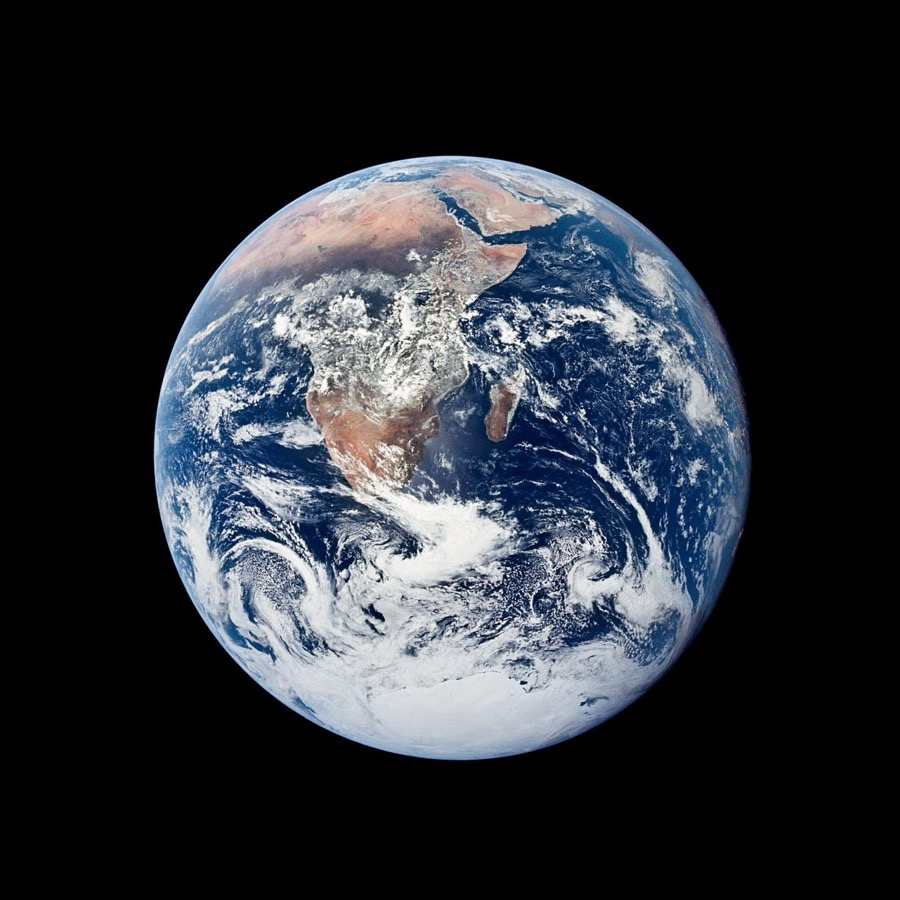
\includegraphics[width=0.55\linewidth]{images/blue-marble-nasa.jpg}
  \caption{Beispielabbildung mit Quellenangabe~\cite{nasa-blue-marble}}
  \label{abb:blue-marble}
\end{figure}

Vektorgrafiken haben gegenüber Screenshots den Vorteil, dass

\begin{itemize}
  \item sie jederzeit editiert werden können,
  \item sie beliebig skaliert werden können, ohne unscharf zu werden,
  \item alle Grafiken einheitlich vergrößert oder verkleinert werden können.
        Das verbessert das Layout ungemein.
\end{itemize}

Abbildungen stehen immer alleinstehend und zentriert. Die Breite wird
relativ zur Textbreite angegeben (\lstinline|width=0.75\linewidth|), damit
sie nie über den Satzspiegel hinausragt. Sollen mehrere Grafiken
nebeneinander stehen, verwendet dafür zwei \lstinline|minipage|-Umgebungen
innerhalb einer \lstinline|figure|.

Die Positionierung übernimmt \LaTeX. Die Angabe \lstinline|[htbp]| erlaubt
es, die Abbildung an die Stelle im Text, an den Seitenanfang, an das
Seitenende oder auf eine eigene Seite zu setzen. Eine Abbildung kann dadurch
auf der Folgeseite landen -- das ist beabsichtigt und kein Fehler.

\subsection{Beschriftungen}

Alle Grafiken und Tabellen sind zu beschriften und mit Quellenangaben zu
versehen. Im Text muss auf jede Abbildung und jede Tabelle Bezug genommen
werden.

Die Beschriftung erfolgt mit \lstinline|\caption| innerhalb der
\lstinline|figure|- bzw.\ \lstinline|table|-Umgebung. Nur so werden
Abbildungs- und Tabellenverzeichnis korrekt geführt. Bei Abbildungen steht
die Beschriftung unter der Grafik, bei Tabellen darüber; die Vorlage stellt
das automatisch richtig ein.

Abbildungen werden mit \enquote{Abb.} und Tabellen mit \enquote{Tab.}
bezeichnet. Auch das erledigt die Vorlage; die Nummerierung läuft
durchgehend und nicht kapitelweise. In englischsprachigen Diplomarbeiten
wird \enquote{Abb.} durch \enquote{Fig.} ersetzt -- dafür genügt die
Klassenoption \lstinline|englisch|.

Unmittelbar nach \lstinline|\caption| gehört ein \lstinline|\label|. Ohne
Label lässt sich die Abbildung später nicht referenzieren. Bewährt hat sich
ein Präfix je Objektart: \lstinline|abb:|, \lstinline|tab:| und
\lstinline|code:|.

\subsection{Querverweise}

Textpassagen, die sich auf andere Kapitel, Grafiken oder Tabellen beziehen,
müssen eine Referenz enthalten. Diese wird mit \lstinline|\ref| erzeugt und
enthält zumindest die Kategorie und die Nummer, also etwa
\lstinline|Abb.~\ref{abb:aufbau}|. Das geschützte Leerzeichen
\lstinline|~| verhindert, dass zwischen Bezeichnung und Nummer umgebrochen
wird.

Liegen referenzierender Text und referenziertes Objekt mehr als eine Seite
auseinander, ist zusätzlich die Seitenzahl mit \lstinline|\pageref|
anzugeben.

Anders als in Word müssen Querverweise und Verzeichnisse nicht manuell
aktualisiert werden. \LaTeX{} löst sie beim Übersetzen auf, benötigt dafür
aber mehrere Durchläufe. \lstinline|latexmk| (bzw.\ \lstinline|make pdf|)
wiederholt den Lauf so lange, bis sich nichts mehr ändert. Meldet das
Protokoll am Ende \enquote{There were undefined references}, fehlt ein
\lstinline|\label| oder es ist falsch geschrieben.

\subsection{Quellenangaben}

In wissenschaftlichen Arbeiten ist es verpflichtend, die Quelle jeder
Aussage anzugeben, die nicht von einem selbst stammt. Der Leser muss die
Möglichkeit haben, die Ausführungen des Autors nachzuprüfen.

Zu diesem Zweck müssen im Text der Diplomarbeit alle verwendeten Quellen
(Fachbücher, Fachzeitschriften, Herstellerunterlagen, Webseiten, \ldots)
angegeben werden. Dies geschieht am Ende des zitierten Textes durch Angabe
der Quelle. Informationen aus Lehrbüchern können als Allgemeinwissen
vorausgesetzt werden und müssen nicht zitiert werden.

Bei inhaltlichen Zitaten, dem Normalfall in technischen Arbeiten, wird der
Inhalt der Quelle nur sinngemäß wiedergegeben.

Bei wörtlichen Zitaten, die in technischen Arbeiten eher selten auftreten,
wird die wörtlich zitierte Textstelle zwischen Anführungszeichen gesetzt,
dahinter steht die Quellenangabe. Eigene Kommentare im Zitat oder
Verkürzungen werden in eckigen Klammern angegeben. Kurze Zitate stehen mit
\lstinline|\zitat| im Fließtext, längere in der Umgebung
\lstinline|zitatfreistehend|.

Beispiel für ein Zitat im Text der Diplomarbeit:
\zitat{[\ldots] kann in diesem Fall eine relationale Datenbank vorteilhaft
eingesetzt werden}~\cite{beispiel-buch}.

Beispiel für ein Zitat als eigener Absatz:

\begin{zitatfreistehend}
  \enquote{The basic guideline for citing online sources is to follow the
  standard citation for the citation, or add the DOI in place of page
  numbers if the source is not paginated.}~\cite{beispiel-artikel}
\end{zitatfreistehend}

Für Diplomarbeiten an der \ac{HTL} Donaustadt ist der IEEE-Zitierstil zu
verwenden. Jeder Quelle wird eine Nummer zugeordnet und in eckigen Klammern
angegeben. Diese Vorlage stellt den Stil bereits ein; zitiert wird mit
\lstinline|\cite{schluessel}|, wobei der Schlüssel aus
\lstinline|references.bib| stammt. Das Quellenverzeichnis wird daraus
automatisch erzeugt und enthält nur tatsächlich zitierte Einträge.

Zum Verwalten der Quellen empfiehlt sich Zotero mit dem Plug-in Better
BibTeX, das \lstinline|references.bib| bei jeder Änderung automatisch neu
exportiert.

Es gibt viele verschiedene Typen von Quellen. Tab.~\ref{tab:quellentypen}
zeigt die häufigsten, den passenden BibTeX-Eintragstyp und die
Informationen, die mindestens enthalten sein sollten.

\begin{table}[htbp]
  \centering
  \caption{Quellentypen}
  \label{tab:quellentypen}
  \begin{tabular}{@{}p{0.28\linewidth}p{0.16\linewidth}p{0.46\linewidth}@{}}
    \toprule
    \tabkopf{Quellentyp} & \tabkopf{Eintragstyp} &
      \tabkopf{wichtigste Informationen} \\
    \midrule
    Buch (auch E-Books, Broschüren) & \lstinline|@book| &
      Autor(en), Titel, Auflage, Verlag, Ort, ISBN \\
    Diplomarbeit, Dissertation & \lstinline|@thesis| &
      Autor(en), Titel, Institution, Ort, Datum \\
    Webseite (auch PDF) & \lstinline|@online| &
      Autor(en), Titel, URL, Abrufdatum (\lstinline|urldate|) \\
    Zeitschriftenartikel & \lstinline|@article| &
      Autor(en), Titel, Publikation, Band, Ausgabe, Seiten, Datum \\
    Verwendung von KI & \lstinline|@online| &
      siehe Anhang und die Vorgaben des Ministeriums~\cite{beispiel-online} \\
    \bottomrule
  \end{tabular}
\end{table}

\subsection{Befehle und Umgebungen}

In Word übernehmen Formatvorlagen das einheitliche Layout. In \LaTeX{}
erfüllen Befehle und Umgebungen dieselbe Aufgabe: Der Text beschreibt, was
etwas \emph{ist}, das Aussehen legt die Dokumentklasse \lstinline|htldon.cls|
zentral fest. Dadurch lässt sich die Formatierung nachträglich an einer
einzigen Stelle ändern.

Die in Tab.~\ref{tab:befehle} aufgeführten Befehle stellen sicher, dass alle
Diplomarbeiten den Richtlinien entsprechen. Sie dürfen nur in begründeten
Ausnahmefällen angepasst werden.

\begin{table}[htbp]
  \centering
  \caption{Befehle und Umgebungen der Vorlage}
  \label{tab:befehle}
  \begin{tabular}{@{}p{0.36\linewidth}p{0.58\linewidth}@{}}
    \toprule
    \tabkopf{Befehl} & \tabkopf{Beschreibung} \\
    \midrule
    \lstinline|\chapter| bis \lstinline|\subsubsection| &
      Kapitelüberschriften mit Dezimalklassifikation. Die ersten drei Ebenen
      erscheinen im Inhaltsverzeichnis, \lstinline|\subsubsection| nicht. \\
    \lstinline|\paragraph| &
      Zwischenüberschrift ohne Nummerierung, nicht im Inhaltsverzeichnis. \\
    \lstinline|\abschnittsautor| &
      Verfasser/in eines Abschnitts, erscheint rechts in der Kopfzeile.
      Format: erster Buchstabe des Vornamens, Punkt, Nachname
      (\enquote{M. Muster}). \\
    \lstinline|\zitat|, \lstinline|zitatfreistehend| &
      Kennzeichnung wörtlicher Zitate im Fließtext bzw.\ als eigener Absatz. \\
    \lstinline|\menue| &
      Menüstrukturen (\menue{Datei / Öffnen}) und Tastatureingaben
      (\menue{Strg + A}). \\
    \lstinline|lstlisting|, \lstinline|\lstinline| &
      Quellcode als eigener Block bzw.\ im Fließtext. \\
    \lstinline|\tabkopf| &
      Kopfzeile einer Tabelle. Der Tabelleninhalt selbst wird von der Klasse
      automatisch auf 10\,pt und linksbündig gestellt. \\
    \lstinline|\ac|, \lstinline|\acp| &
      Abkürzung, beim ersten Auftreten ausgeschrieben, im Plural mit
      \lstinline|\acp|. \\
    \lstinline|\cite|, \lstinline|\ref|, \lstinline|\pageref| &
      Quellenangabe, Querverweis, Seitenverweis. \\
    \bottomrule
  \end{tabular}
\end{table}

Überschriften der Kapitel müssen kurz, präzise und selbsterklärend sein.
Beispiele für unzureichende Überschriften: \enquote{5.3 Aufbau},
\enquote{5.3 Messergebnis}, \enquote{5.3 Beispiel}.

Bei Unterüberschriften gilt:

\begin{itemize}
  \item Es muss mindestens zwei Unterpunkte geben. Ein Abschnitt 3.2.1 darf
        daher nicht existieren, wenn kein 3.2.2 folgt.
  \item Unterpunkte sollten inhaltlich ausreichend gefüllt sein und
        mindestens eine halbe Seite umfassen.
  \item Unterpunkte, die lediglich aus einem einzelnen Satz bestehen, werden
        besser als Aufzählung dargestellt.
\end{itemize}

Für die Darstellung von Quellcode gilt:

\begin{itemize}
  \item Umfang:
        \begin{itemize}
          \item Der vollständige Sourcecode gehört ausschließlich auf das
                elektronische Speichermedium.
          \item Im Dokument selbst sollen nur wesentliche Ausschnitte
                aufgenommen werden.
        \end{itemize}
  \item Formatierung: Schriftart und Schriftgröße gibt die
        \lstinline|lstlisting|-Umgebung vor, der Zeilenabstand ist dort
        einzeilig. Die Sprache wird mit
        \lstinline|[language=Python]| angegeben, damit die
        Syntaxhervorhebung stimmt.
  \item Inhaltliche Anforderungen: Der Sourcecode muss ausreichend
        kommentiert sein.
  \item Verwendung im Fließtext: Wird Sourcecode im Text erwähnt, ist
        \lstinline|\lstinline| zu verwenden. Zusätzliche Anführungszeichen
        sind nicht erforderlich. Beispiel: Mit dem Befehl
        \lstinline|ShowModal| wird ein Frame geöffnet.
\end{itemize}

\section{Beschreibung der Kapitel}

\subsection{Titelseite}

Die Titelseite wird vollständig aus \lstinline|metadata.tex| erzeugt. Dort
sind einzutragen:

\begin{itemize}
  \item der Titel der Diplomarbeit mit \lstinline|\titel|. Er wird
        automatisch in die Kopfzeile übernommen.
  \item ein Projektlogo, Bild oder eine Zeichnung mit
        \lstinline|\projektlogo|.
  \item alle Verfasser/innen mit \lstinline|\teammitglied| und die
        Betreuung mit \lstinline|\betreuung|.
  \item Schuljahr, Abteilung und Klasse.
\end{itemize}

Falls alle Verfasser/innen oder Betreuer/innen dasselbe Geschlecht haben,
kann die geschlechtsspezifische Form verwendet werden; dafür ist das
optionale Argument von \lstinline|\betreuung| vorgesehen.

\subsection{Verfassererklärung}

In der Verfassererklärung bekennen sich die Verfasser/innen zu einem
wissenschaftlichen Arbeitsstil. Sollten im Nachhinein grobe Verstöße dagegen
aufgedeckt werden, kann die Arbeit für ungültig erklärt und der Abschluss
revidiert werden.

Die Erklärung erzeugt \lstinline|\eigenstaendigkeitserklaerung|. Je
Teammitglied entsteht automatisch eine Unterschriftszeile. Zu ergänzen sind
gegebenenfalls Kooperationen mit Firmen und Sperrvermerke.

\subsection{Problemstellung}

Die Seite \enquote{Problemstellung} wird durch den eingescannten Antrag (mit
allen Stempeln und Unterschriften) vollflächig ersetzt. Dazu wird in
\lstinline|frontmatter/problem-statement.tex| das Scan-PDF eingebunden.

\subsection{Kurzfassung bzw.\ Abstract}

Die Kurzfassung bzw.\ der Abstract soll kurz, prägnant und verständlich den
Inhalt der Arbeit wiedergeben: Zielsetzung, Ablauf, wichtigste Erkenntnisse,
wesentliche Merkmale des realisierten Produkts, Schlussfolgerungen und
Ausblick. Beide sind als eigenständiges Dokument zu konzipieren, das
unabhängig von der Diplomarbeit gelesen und verstanden werden kann, und
sollen in Deutsch und Englisch jeweils nicht mehr als eine Seite umfassen.

\subsection{Inhaltsverzeichnis}

Das Inhaltsverzeichnis wird automatisch aus den Überschriften erstellt. Es
zeigt die ersten drei Ebenen, der Text steht linksbündig, die Seitenzahlen
rechtsbündig, als Füllzeichen dienen Punkte. Eine manuelle Aktualisierung
ist nicht nötig.

\subsection{Die weiteren Kapitel}

Die Kapitel Projektplanung, Technische Grundlagen, Praktische Realisierung
sowie Evaluierung und Ergebnisse beschreiben die Diplomarbeit im Detail.

Für die Beurteilung ist es wichtig, den/die Verfasser/in zu kennen. Daher
ist dieser Hinweis auf jeder Seite rechtsbündig in der Kopfzeile zu
vermerken. Dafür wird \lstinline|\abschnittsautor| direkt nach der
Überschrift gesetzt; der Eintrag gilt ab dort bis zur nächsten Angabe.
Haben mehrere Personen gemeinsam an einem Abschnitt gearbeitet, sind alle zu
nennen, durch Komma getrennt:
\lstinline|\abschnittsautor{A. Erste, B. Zweite}|.

Die Projektplanung soll die systematische Durchführung der Diplomarbeit
innerhalb des Projektteams beschreiben. Dabei sollen geplante Ziele und
tatsächlich erreichte Ergebnisse miteinander verglichen und die Unterschiede
reflektiert werden. Beim klassischen Wasserfall-Projektmanagement können
etwa die Meilensteine als Referenz dienen, bei agiler Projektorganisation
die Sprint-Reviews.

Im Kapitel Technische Grundlagen finden sich alle für das unmittelbare
technische Verständnis der Diplomarbeit relevanten Inhalte. Hier wird
insbesondere auf korrekte Zitate und den sorgfältigen Einsatz von Quellen
geachtet.

Das Kapitel Praktische Realisierung enthält die praktischen Eigenleistungen
der Diplomarbeit. Dabei sollen die Vorgänge und Untersuchungen beschrieben
und nachvollziehbar dokumentiert werden.

Im Kapitel Evaluierung und Ergebnisse erfolgt die Darstellung und Bewertung
der abschließenden Arbeit. Hier soll ebenso, sofern vorhanden, das
Endprodukt bzw.\ der Prototyp präsentiert und beschrieben werden.

\subsection{Anhang}

Im Anhang können alle Informationen gesammelt werden, die zwar zur
Diplomarbeit gehören, jedoch im Inhaltsteil den Rahmen gesprengt hätten.
Dazu zählen wichtige Notizen (z.\,B. Gesprächsprotokolle), Normen,
Schnittstellendefinitionen oder Präsentationen. Weiters soll der Anhang den
Inhalt eines beigefügten elektronischen Speichermediums sowie einen
einseitigen Lebenslauf jedes Teammitglieds enthalten.

Verpflichtend ist außerdem die Dokumentation aller eingesetzten KI-basierten
Hilfsmittel. Dafür ist \lstinline|appendix/ai-tools.tex| vorgesehen.
| zu löschen. Die Einträge
im Inhaltsverzeichnis und in den übrigen Verzeichnissen verschwinden beim
nächsten Übersetzen von selbst.

\subsection{Abgabe der Diplomarbeit}

Die Diplomarbeit ist in gedruckter bzw.\ gebundener Form und in digitaler
Form vorzulegen. Dem Abteilungsvorstand sind zwei geheftete Exemplare (ein
Belegexemplar und ein Beurteilungsexemplar für den/die Betreuer/in) zu
übergeben.

Nach erfolgter Beurteilung geht das Beurteilungsexemplar temporär zurück an
die Diplomarbeitsgruppe. Nun können letzte Korrekturen (ohne
Beurteilungsrelevanz) vorgenommen werden. Anschließend wird die Arbeit erneut
ausgedruckt und gesammelt zur Bindung außer Haus gegeben. Weitere Exemplare
für Kooperationspartner (Firmen, Institutionen) oder Projektteilnehmer können
in diesem Zusammenhang erstellt werden.

\subsection{Grafiken}

Abbildungen müssen in gut lesbarer Bildqualität eingefügt werden. Grafiken
sollten am besten in einem vektorbasierten Zeichenprogramm (z.\,B. Inkscape,
draw.io) erstellt und als PDF exportiert werden; PDF und PNG lassen sich
direkt einbinden, SVG nicht. Alle Bilddateien gehören in den Ordner
\lstinline|images/|.

\begin{lstlisting}[language={[LaTeX]TeX}, caption={Eine Abbildung einbinden},
                   label=code:abbildung]
\begin{figure}[htbp]
  \centering
  
\includegraphics[width=0.75\linewidth]{images/example-figure.pdf}
  \caption{Aufbau des Systems}
  \label{abb:aufbau}
\end{figure}
\end{lstlisting}

Abb.~\ref{abb:blue-marble} zeigt, wie das Ergebnis aussieht. Stammt die
Grafik nicht von euch selbst, gehört die Quelle in die Beschriftung.

\begin{figure}[htbp]
  \centering
  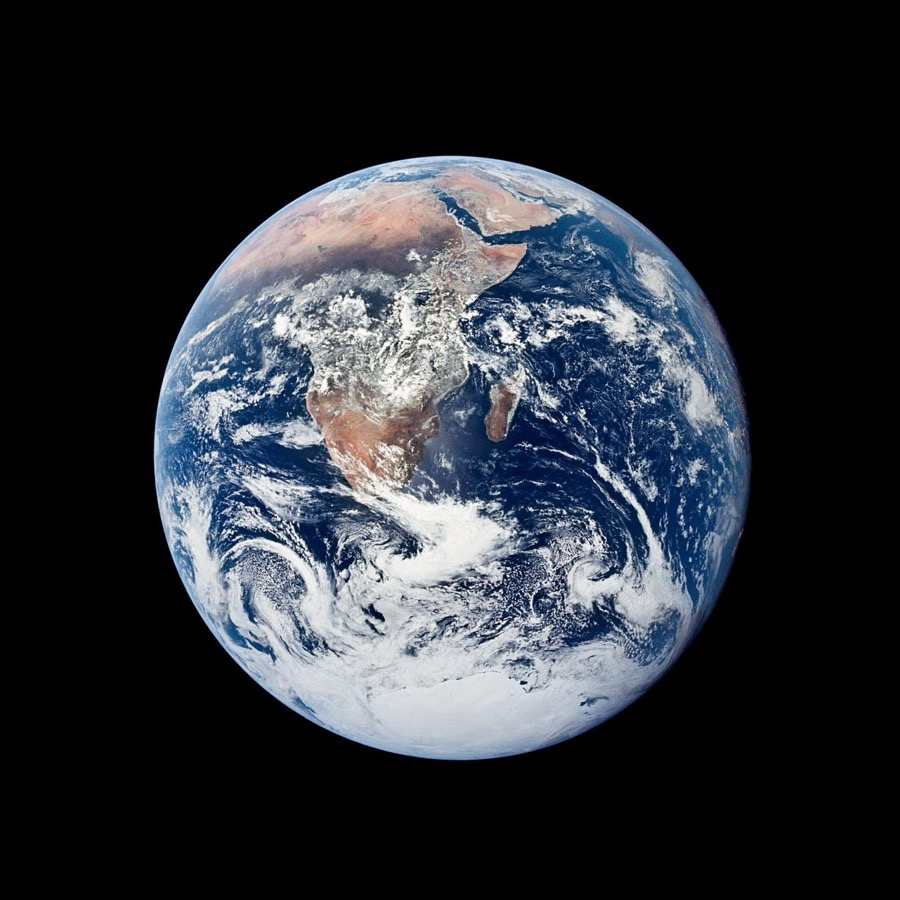
\includegraphics[width=0.55\linewidth]{images/blue-marble-nasa.jpg}
  \caption{Beispielabbildung mit Quellenangabe~\cite{nasa-blue-marble}}
  \label{abb:blue-marble}
\end{figure}

Vektorgrafiken haben gegenüber Screenshots den Vorteil, dass

\begin{itemize}
  \item sie jederzeit editiert werden können,
  \item sie beliebig skaliert werden können, ohne unscharf zu werden,
  \item alle Grafiken einheitlich vergrößert oder verkleinert werden können.
        Das verbessert das Layout ungemein.
\end{itemize}

Abbildungen stehen immer alleinstehend und zentriert. Die Breite wird
relativ zur Textbreite angegeben (\lstinline|width=0.75\linewidth|), damit
sie nie über den Satzspiegel hinausragt. Sollen mehrere Grafiken
nebeneinander stehen, verwendet dafür zwei \lstinline|minipage|-Umgebungen
innerhalb einer \lstinline|figure|.

Die Positionierung übernimmt \LaTeX. Die Angabe \lstinline|[htbp]| erlaubt
es, die Abbildung an die Stelle im Text, an den Seitenanfang, an das
Seitenende oder auf eine eigene Seite zu setzen. Eine Abbildung kann dadurch
auf der Folgeseite landen -- das ist beabsichtigt und kein Fehler.

\subsection{Beschriftungen}

Alle Grafiken und Tabellen sind zu beschriften und mit Quellenangaben zu
versehen. Im Text muss auf jede Abbildung und jede Tabelle Bezug genommen
werden.

Die Beschriftung erfolgt mit \lstinline|\caption| innerhalb der
\lstinline|figure|- bzw.\ \lstinline|table|-Umgebung. Nur so werden
Abbildungs- und Tabellenverzeichnis korrekt geführt. Bei Abbildungen steht
die Beschriftung unter der Grafik, bei Tabellen darüber; die Vorlage stellt
das automatisch richtig ein.

Abbildungen werden mit \enquote{Abb.} und Tabellen mit \enquote{Tab.}
bezeichnet. Auch das erledigt die Vorlage; die Nummerierung läuft
durchgehend und nicht kapitelweise. In englischsprachigen Diplomarbeiten
wird \enquote{Abb.} durch \enquote{Fig.} ersetzt -- dafür genügt die
Klassenoption \lstinline|englisch|.

Unmittelbar nach \lstinline|\caption| gehört ein \lstinline|\label|. Ohne
Label lässt sich die Abbildung später nicht referenzieren. Bewährt hat sich
ein Präfix je Objektart: \lstinline|abb:|, \lstinline|tab:| und
\lstinline|code:|.

\subsection{Querverweise}

Textpassagen, die sich auf andere Kapitel, Grafiken oder Tabellen beziehen,
müssen eine Referenz enthalten. Diese wird mit \lstinline|\ref| erzeugt und
enthält zumindest die Kategorie und die Nummer, also etwa
\lstinline|Abb.~\ref{abb:aufbau}|. Das geschützte Leerzeichen
\lstinline|~| verhindert, dass zwischen Bezeichnung und Nummer umgebrochen
wird.

Liegen referenzierender Text und referenziertes Objekt mehr als eine Seite
auseinander, ist zusätzlich die Seitenzahl mit \lstinline|\pageref|
anzugeben.

Anders als in Word müssen Querverweise und Verzeichnisse nicht manuell
aktualisiert werden. \LaTeX{} löst sie beim Übersetzen auf, benötigt dafür
aber mehrere Durchläufe. \lstinline|latexmk| (bzw.\ \lstinline|make pdf|)
wiederholt den Lauf so lange, bis sich nichts mehr ändert. Meldet das
Protokoll am Ende \enquote{There were undefined references}, fehlt ein
\lstinline|\label| oder es ist falsch geschrieben.

\subsection{Quellenangaben}

In wissenschaftlichen Arbeiten ist es verpflichtend, die Quelle jeder
Aussage anzugeben, die nicht von einem selbst stammt. Der Leser muss die
Möglichkeit haben, die Ausführungen des Autors nachzuprüfen.

Zu diesem Zweck müssen im Text der Diplomarbeit alle verwendeten Quellen
(Fachbücher, Fachzeitschriften, Herstellerunterlagen, Webseiten, \ldots)
angegeben werden. Dies geschieht am Ende des zitierten Textes durch Angabe
der Quelle. Informationen aus Lehrbüchern können als Allgemeinwissen
vorausgesetzt werden und müssen nicht zitiert werden.

Bei inhaltlichen Zitaten, dem Normalfall in technischen Arbeiten, wird der
Inhalt der Quelle nur sinngemäß wiedergegeben.

Bei wörtlichen Zitaten, die in technischen Arbeiten eher selten auftreten,
wird die wörtlich zitierte Textstelle zwischen Anführungszeichen gesetzt,
dahinter steht die Quellenangabe. Eigene Kommentare im Zitat oder
Verkürzungen werden in eckigen Klammern angegeben. Kurze Zitate stehen mit
\lstinline|\zitat| im Fließtext, längere in der Umgebung
\lstinline|zitatfreistehend|.

Beispiel für ein Zitat im Text der Diplomarbeit:
\zitat{[\ldots] kann in diesem Fall eine relationale Datenbank vorteilhaft
eingesetzt werden}~\cite{beispiel-buch}.

Beispiel für ein Zitat als eigener Absatz:

\begin{zitatfreistehend}
  \enquote{The basic guideline for citing online sources is to follow the
  standard citation for the citation, or add the DOI in place of page
  numbers if the source is not paginated.}~\cite{beispiel-artikel}
\end{zitatfreistehend}

Für Diplomarbeiten an der \ac{HTL} Donaustadt ist der IEEE-Zitierstil zu
verwenden. Jeder Quelle wird eine Nummer zugeordnet und in eckigen Klammern
angegeben. Diese Vorlage stellt den Stil bereits ein; zitiert wird mit
\lstinline|\cite{schluessel}|, wobei der Schlüssel aus
\lstinline|references.bib| stammt. Das Quellenverzeichnis wird daraus
automatisch erzeugt und enthält nur tatsächlich zitierte Einträge.

Zum Verwalten der Quellen empfiehlt sich Zotero mit dem Plug-in Better
BibTeX, das \lstinline|references.bib| bei jeder Änderung automatisch neu
exportiert.

Es gibt viele verschiedene Typen von Quellen. Tab.~\ref{tab:quellentypen}
zeigt die häufigsten, den passenden BibTeX-Eintragstyp und die
Informationen, die mindestens enthalten sein sollten.

\begin{table}[htbp]
  \centering
  \caption{Quellentypen}
  \label{tab:quellentypen}
  \begin{tabular}{@{}p{0.28\linewidth}p{0.16\linewidth}p{0.46\linewidth}@{}}
    \toprule
    \tabkopf{Quellentyp} & \tabkopf{Eintragstyp} &
      \tabkopf{wichtigste Informationen} \\
    \midrule
    Buch (auch E-Books, Broschüren) & \lstinline|@book| &
      Autor(en), Titel, Auflage, Verlag, Ort, ISBN \\
    Diplomarbeit, Dissertation & \lstinline|@thesis| &
      Autor(en), Titel, Institution, Ort, Datum \\
    Webseite (auch PDF) & \lstinline|@online| &
      Autor(en), Titel, URL, Abrufdatum (\lstinline|urldate|) \\
    Zeitschriftenartikel & \lstinline|@article| &
      Autor(en), Titel, Publikation, Band, Ausgabe, Seiten, Datum \\
    Verwendung von KI & \lstinline|@online| &
      siehe Anhang und die Vorgaben des Ministeriums~\cite{beispiel-online} \\
    \bottomrule
  \end{tabular}
\end{table}

\subsection{Befehle und Umgebungen}

In Word übernehmen Formatvorlagen das einheitliche Layout. In \LaTeX{}
erfüllen Befehle und Umgebungen dieselbe Aufgabe: Der Text beschreibt, was
etwas \emph{ist}, das Aussehen legt die Dokumentklasse \lstinline|htldon.cls|
zentral fest. Dadurch lässt sich die Formatierung nachträglich an einer
einzigen Stelle ändern.

Die in Tab.~\ref{tab:befehle} aufgeführten Befehle stellen sicher, dass alle
Diplomarbeiten den Richtlinien entsprechen. Sie dürfen nur in begründeten
Ausnahmefällen angepasst werden.

\begin{table}[htbp]
  \centering
  \caption{Befehle und Umgebungen der Vorlage}
  \label{tab:befehle}
  \begin{tabular}{@{}p{0.36\linewidth}p{0.58\linewidth}@{}}
    \toprule
    \tabkopf{Befehl} & \tabkopf{Beschreibung} \\
    \midrule
    \lstinline|\chapter| bis \lstinline|\subsubsection| &
      Kapitelüberschriften mit Dezimalklassifikation. Die ersten drei Ebenen
      erscheinen im Inhaltsverzeichnis, \lstinline|\subsubsection| nicht. \\
    \lstinline|\paragraph| &
      Zwischenüberschrift ohne Nummerierung, nicht im Inhaltsverzeichnis. \\
    \lstinline|\abschnittsautor| &
      Verfasser/in eines Abschnitts, erscheint rechts in der Kopfzeile.
      Format: erster Buchstabe des Vornamens, Punkt, Nachname
      (\enquote{M. Muster}). \\
    \lstinline|\zitat|, \lstinline|zitatfreistehend| &
      Kennzeichnung wörtlicher Zitate im Fließtext bzw.\ als eigener Absatz. \\
    \lstinline|\menue| &
      Menüstrukturen (\menue{Datei / Öffnen}) und Tastatureingaben
      (\menue{Strg + A}). \\
    \lstinline|lstlisting|, \lstinline|\lstinline| &
      Quellcode als eigener Block bzw.\ im Fließtext. \\
    \lstinline|\tabkopf| &
      Kopfzeile einer Tabelle. Der Tabelleninhalt selbst wird von der Klasse
      automatisch auf 10\,pt und linksbündig gestellt. \\
    \lstinline|\ac|, \lstinline|\acp| &
      Abkürzung, beim ersten Auftreten ausgeschrieben, im Plural mit
      \lstinline|\acp|. \\
    \lstinline|\cite|, \lstinline|\ref|, \lstinline|\pageref| &
      Quellenangabe, Querverweis, Seitenverweis. \\
    \bottomrule
  \end{tabular}
\end{table}

Überschriften der Kapitel müssen kurz, präzise und selbsterklärend sein.
Beispiele für unzureichende Überschriften: \enquote{5.3 Aufbau},
\enquote{5.3 Messergebnis}, \enquote{5.3 Beispiel}.

Bei Unterüberschriften gilt:

\begin{itemize}
  \item Es muss mindestens zwei Unterpunkte geben. Ein Abschnitt 3.2.1 darf
        daher nicht existieren, wenn kein 3.2.2 folgt.
  \item Unterpunkte sollten inhaltlich ausreichend gefüllt sein und
        mindestens eine halbe Seite umfassen.
  \item Unterpunkte, die lediglich aus einem einzelnen Satz bestehen, werden
        besser als Aufzählung dargestellt.
\end{itemize}

Für die Darstellung von Quellcode gilt:

\begin{itemize}
  \item Umfang:
        \begin{itemize}
          \item Der vollständige Sourcecode gehört ausschließlich auf das
                elektronische Speichermedium.
          \item Im Dokument selbst sollen nur wesentliche Ausschnitte
                aufgenommen werden.
        \end{itemize}
  \item Formatierung: Schriftart und Schriftgröße gibt die
        \lstinline|lstlisting|-Umgebung vor, der Zeilenabstand ist dort
        einzeilig. Die Sprache wird mit
        \lstinline|[language=Python]| angegeben, damit die
        Syntaxhervorhebung stimmt.
  \item Inhaltliche Anforderungen: Der Sourcecode muss ausreichend
        kommentiert sein.
  \item Verwendung im Fließtext: Wird Sourcecode im Text erwähnt, ist
        \lstinline|\lstinline| zu verwenden. Zusätzliche Anführungszeichen
        sind nicht erforderlich. Beispiel: Mit dem Befehl
        \lstinline|ShowModal| wird ein Frame geöffnet.
\end{itemize}

\section{Beschreibung der Kapitel}

\subsection{Titelseite}

Die Titelseite wird vollständig aus \lstinline|metadata.tex| erzeugt. Dort
sind einzutragen:

\begin{itemize}
  \item der Titel der Diplomarbeit mit \lstinline|\titel|. Er wird
        automatisch in die Kopfzeile übernommen.
  \item ein Projektlogo, Bild oder eine Zeichnung mit
        \lstinline|\projektlogo|.
  \item alle Verfasser/innen mit \lstinline|\teammitglied| und die
        Betreuung mit \lstinline|\betreuung|.
  \item Schuljahr, Abteilung und Klasse.
\end{itemize}

Falls alle Verfasser/innen oder Betreuer/innen dasselbe Geschlecht haben,
kann die geschlechtsspezifische Form verwendet werden; dafür ist das
optionale Argument von \lstinline|\betreuung| vorgesehen.

\subsection{Verfassererklärung}

In der Verfassererklärung bekennen sich die Verfasser/innen zu einem
wissenschaftlichen Arbeitsstil. Sollten im Nachhinein grobe Verstöße dagegen
aufgedeckt werden, kann die Arbeit für ungültig erklärt und der Abschluss
revidiert werden.

Die Erklärung erzeugt \lstinline|\eigenstaendigkeitserklaerung|. Je
Teammitglied entsteht automatisch eine Unterschriftszeile. Zu ergänzen sind
gegebenenfalls Kooperationen mit Firmen und Sperrvermerke.

\subsection{Problemstellung}

Die Seite \enquote{Problemstellung} wird durch den eingescannten Antrag (mit
allen Stempeln und Unterschriften) vollflächig ersetzt. Dazu wird in
\lstinline|frontmatter/problem-statement.tex| das Scan-PDF eingebunden.

\subsection{Kurzfassung bzw.\ Abstract}

Die Kurzfassung bzw.\ der Abstract soll kurz, prägnant und verständlich den
Inhalt der Arbeit wiedergeben: Zielsetzung, Ablauf, wichtigste Erkenntnisse,
wesentliche Merkmale des realisierten Produkts, Schlussfolgerungen und
Ausblick. Beide sind als eigenständiges Dokument zu konzipieren, das
unabhängig von der Diplomarbeit gelesen und verstanden werden kann, und
sollen in Deutsch und Englisch jeweils nicht mehr als eine Seite umfassen.

\subsection{Inhaltsverzeichnis}

Das Inhaltsverzeichnis wird automatisch aus den Überschriften erstellt. Es
zeigt die ersten drei Ebenen, der Text steht linksbündig, die Seitenzahlen
rechtsbündig, als Füllzeichen dienen Punkte. Eine manuelle Aktualisierung
ist nicht nötig.

\subsection{Die weiteren Kapitel}

Die Kapitel Projektplanung, Technische Grundlagen, Praktische Realisierung
sowie Evaluierung und Ergebnisse beschreiben die Diplomarbeit im Detail.

Für die Beurteilung ist es wichtig, den/die Verfasser/in zu kennen. Daher
ist dieser Hinweis auf jeder Seite rechtsbündig in der Kopfzeile zu
vermerken. Dafür wird \lstinline|\abschnittsautor| direkt nach der
Überschrift gesetzt; der Eintrag gilt ab dort bis zur nächsten Angabe.
Haben mehrere Personen gemeinsam an einem Abschnitt gearbeitet, sind alle zu
nennen, durch Komma getrennt:
\lstinline|\abschnittsautor{A. Erste, B. Zweite}|.

Die Projektplanung soll die systematische Durchführung der Diplomarbeit
innerhalb des Projektteams beschreiben. Dabei sollen geplante Ziele und
tatsächlich erreichte Ergebnisse miteinander verglichen und die Unterschiede
reflektiert werden. Beim klassischen Wasserfall-Projektmanagement können
etwa die Meilensteine als Referenz dienen, bei agiler Projektorganisation
die Sprint-Reviews.

Im Kapitel Technische Grundlagen finden sich alle für das unmittelbare
technische Verständnis der Diplomarbeit relevanten Inhalte. Hier wird
insbesondere auf korrekte Zitate und den sorgfältigen Einsatz von Quellen
geachtet.

Das Kapitel Praktische Realisierung enthält die praktischen Eigenleistungen
der Diplomarbeit. Dabei sollen die Vorgänge und Untersuchungen beschrieben
und nachvollziehbar dokumentiert werden.

Im Kapitel Evaluierung und Ergebnisse erfolgt die Darstellung und Bewertung
der abschließenden Arbeit. Hier soll ebenso, sofern vorhanden, das
Endprodukt bzw.\ der Prototyp präsentiert und beschrieben werden.

\subsection{Anhang}

Im Anhang können alle Informationen gesammelt werden, die zwar zur
Diplomarbeit gehören, jedoch im Inhaltsteil den Rahmen gesprengt hätten.
Dazu zählen wichtige Notizen (z.\,B. Gesprächsprotokolle), Normen,
Schnittstellendefinitionen oder Präsentationen. Weiters soll der Anhang den
Inhalt eines beigefügten elektronischen Speichermediums sowie einen
einseitigen Lebenslauf jedes Teammitglieds enthalten.

Verpflichtend ist außerdem die Dokumentation aller eingesetzten KI-basierten
Hilfsmittel. Dafür ist \lstinline|appendix/ai-tools.tex| vorgesehen.
